\documentclass{VUMIFPSkursinis}
\usepackage{algorithmicx}
\usepackage{algorithm}
\usepackage{algpseudocode}
\usepackage{amsfonts}
\usepackage{amsmath}
\usepackage{array}
\usepackage{bm}
\usepackage{caption}
\usepackage{color}
\usepackage{float}
\usepackage{graphicx}
\usepackage{listings}
\usepackage{subfig}
\usepackage{wrapfig}
\usepackage{booktabs}
\usepackage{lscape}
\usepackage{longtable}
\usepackage{verbatim}


\usepackage{enumitem}
%PAKEISTA, tarpai tarp sąrašo elementų
\setitemize{noitemsep,topsep=0pt,parsep=0pt,partopsep=0pt}
\setenumerate{noitemsep,topsep=0pt,parsep=0pt,partopsep=0pt}

% Titulinio aprašas
\university{Vilniaus universitetas}
\faculty{Matematikos ir informatikos fakultetas}
\department{Programų sistemų katedra}
\papertype{Programų sistemų inžinerijos laboratorinis darbas}
\title{Biblioteka}
%\titleineng{Library}
\status{2 kurso 5 grupės }
\author{Šarūnas Kazimieras Buteikis}
\secondauthor{Modestas Dulevičius}
\thirdauthor{Paulius Grigaliūnas}
\fourthauthor{Albert Jurkoit}
\fifthauthor{Karolis Staskevičius}

\supervisor{dr. Vytautas Valaitis}
\date{Vilnius – \the\year}

% Nustatymai
% \setmainfont{Palemonas}   % Pakeisti teksto šriftą į Palemonas (turi būti įdiegtas sistemoje)

\begin{document}
	
% PAKEISTA	
\maketitle
\cleardoublepage\pagenumbering{arabic}
\setcounter{page}{2}
\sectionnonum{Anotacija}
Šiame dokumente, remiantis anktesnėmis dokumento versijomis, buvo atliktos toliau nurodytos ICONIX proceso veiklos iki ir vykstant implementacijai:\\
	\begin{itemize}
    	\item Galutinai apibrėžti reikalavimai sistemai.
    	\item Patobulintas struktūrinis dalykinės srities modelis.
    	\item Apibrėžtos sistemos atliekamos užduotys.
    	\item Patikslinta techninė sistemos architektūra.
        \item Sukurtas testavimo planas ir scenarijai.
        \item Papildytas klaidų, rastų atliekant kritinę projekto peržiūrą, sąrašas. 
	\end{itemize}
%TURINYS
\tableofcontents{}

\sectionnonum{Įvadas}

Kuriant šį darbą buvo remtasi dėstytojo puslapyje nurodyta dokumento struktūra \cite{1} bei Don Rosenberg "Use Case Driven Object Modeling with UML Theory and Practice."\cite{2}  knyga.
%FIXME

\noindent
\textbf{Dalykinė sritis}\\ 
Skaitytojui ir bibliotekos personalui patogi naudoti programinė įranga, suteikianti galimybę skaitytojams iš namų užsirezervuoti norimą knygą.\\ 
\textbf{Darbo pagrindas}\\
Dokumentas parengtas kaip programų sistemų inžinerijos laboratorinis darbas\\
\pagebreak

\sectionnonum{Žodynas/Esybių sąrašas}
\noindent
ES1 Biblioteka - įstaiga nusipirkusi ir naudojanti šiame dokumente minėtą programinę įrangą.\\
ES2 Bibliotekos darbuotojas - bibliotekininkas arba kitas darbuotojas atsakingas už bendravimą su skaitytojais, knygų grąžinimą ir skolinimą.\\
ES3 Skaitytojas - asmuo kuris skolinasi arba bent turi galimybę skolintis knygas iš bibliotekos naudojantis mūsų programinę įrangą.\\
ES4 Knyga - bibliotekos skolinamas objektas skaitytojams. Knygos gali būti rezervuojamos. Kiekvienas knygos egzempliorius turi savo ID numerį.\\
ES5 Rezervavimas - užtikrinimas, kad knyga artimu laiku bus paskolinta skaitytojui kuris ją rezervavo.\\
ES6 Grąžinimas - veiksmas, kuriuo knyga grąžinama į biblioteką ir vėl yra prieinama skaitytojams.\\
ES7 Bauda - mokestis skiriamas skaitytojui už pavėluotą grąžinti arba pamestą knygą.\\
ES8 ID - unikalus knygos arba skaitytojo numeris padedantis identifikuoti.\\
ES9 Programėlė - skaitytojo naudojama programinės įrangos dalis leidžianti ieškoti, rezervuoti knygas ir suteikianti kita skaitytojui naudingą funkcionalumą.\\
ES10 Administratorius - bibliotekos darbuotojas arba mūsų kompanijos inžinierius turintis daugiau įgaliojimų programinei įrangai tvarkyti ir prižiūrėti, nei įprasti bibliotekos darbuotojai.\\
ES11 Prisijungimo duomenys - duomenys skirti suteikti prieigą prie tam tikro kiekio programos funkcionalumo.\\
ES12 Skaitytojo duomenys - visa informacija kuri yra saugoma apie konkretų skaitytoją, išskyrus prisijungimo duomenis.\\
ES13 Skolinimas - veiksmas, kuriuo skaitytojas gauną knygą iš bibliotekos ir turi teisę ją turėti iki nurodyto laiko.\\
ES15 Vartotojo sesija - prisijungimas, kuris leidžia naudotis didžiąją dalimi programėlės funkcionalumo. Nutraukiama vartotojui atsijungus.\\
ES16 Duomenų bazė (arba duombazė) - serveris laikantis informaciją apie prisijungimo duomenis, knygas ir kitą su sistema susijusią informaciją.
ES17 Skolinimas - knygos perleidimas skaitytojui tam tikram laiko tarpui.
\newpage

% * <Karolis> 2018-05-30T15:52:49.138Z:
% 
% > \part{Programos reikalavimai}
% > Šioje dalyje bus pateikti reikalavimai sistemai.
% 
% Išėmiau, nes buvo vienintelė dalis(part) visoje dokumentacijoje
%
% ^.

\section{Funkciniai reikalavimai}
Pagrindinių sistemos funkcijų reikalavimai

\subsection{Programos kliento dalies funkciniai reikalavimai}
Reikalavimai skirti apibrėžti programos kliento dalį.

\subsubsection{Vartotojo paskyros sukūrimas }
\noindent
 \vspace{5mm}
  \begin{tabular}{ | p{1,5cm} | p{11,8cm} | p{2,3cm} |}
    \hline
   \multicolumn{2}{|l|}{FR 1. Pradiniai duomenys} &Svarba  \\ \hline 
   FR 1.1 & Vatotojo Vardas (simbolių eilutė iki 15 simbolių) & Būtinas\\ \hline
    FR 1.2& Slaptažodis (simbolių eilutė iki 20 simbolių) &Būtinas \\ \hline
    FR 1.3  & Adresas (simbolių eilutė iki 30 simbolių)  &Būtinas\\
\hline
 FR 1.4 &  Pašto kodas (simbolių eilutė iki 5 simbolių) &  Būtinas\\   \hline
 FR 1.5 &  Tikras Vartotojo Vardas (simbolių eilutė iki 50 simbolių) &  Pageidautinas\\   \hline 
 FR 1.6 &  Telefono numeris (simbolių eilutė iki 12 simbolių) &  Būtinas\\   \hline
    \end{tabular}
 \vspace{5mm}
  \begin{tabular}{ | p{1,5cm} | p{11,8cm} | p{2,3cm} |}
    \hline
   \multicolumn{2}{|l|}{FR 2. Veiksmai} &Svarba  \\ \hline 
  FR 2.1 &Įvesti registracijos duomenis į atitinkamus laukus & Būtinas\\ \hline
    FR 2.2& Patvirtinti registraciją iššokusiame langelyje &Būtinas \\ \hline
    \end{tabular} 
\vspace{5mm}
  \begin{tabular}{ | p{1,5cm} | p{11,8cm} | p{2,3cm} |}
    \hline
   \multicolumn{2}{|l|}{FR 3. Alternatyvūs scenarijai} &Svarba  \\ \hline 
  FR 3.1 &Jeigu vartotojas įveda netinkamus duomenis arba toks vartotojo vardas jau užregistruotas, išvedama informacija apie tinkamą duomenų įvedimą. & Būtinas\\ \hline
     FR 3.2&  Jei vartotojas nepatvirtina registracijos negalės buti užregistruotas&Būtinas \\ \hline
    \end{tabular}
 \vspace{5mm}
  \begin{tabular}{ | p{1,5cm} | p{11,8cm} | p{2,3cm} |}
    \hline
   \multicolumn{2}{|l|}{ FR 4. Reikalavimai} &Svarba  \\ \hline 
   FR 4.1 &  Galima naudoti visas raidės priklausančias Unicode simboliams & Būtinas\\ \hline
    FR 4.2& Visi registracijos formos laukai turi būti užpildyti &Būtinas \\ \hline
    FR 4.3 &  Vartotojo įvedamas slaptažodis negali būti matomas &  Būtinas\\
    \hline
    FR 4.4  & Telefono numeris turi prasidėti +370  &Būtinas\\
    \hline
    \end{tabular}

 

\subsubsection{Prisijungimas prie programos}
\noindent
 \vspace{5mm}
 \begin{tabular}{ | p{1,5cm} | p{11,8cm} | p{2,3cm} |}
    \hline
    \multicolumn{2}{|l|}{  FR 6. Pradiniai duomenys} &Svarba  \\ \hline 
  FR 6.1&  Vartotojo vardas (simbolių eilutė iki 20 simbolių)&  Būtinas\\ \hline
  FR 6.2&  Slaptažodis (simbolių eilutė iki 20 simbolių)&  Būtinas\\ \hline
  FR 6.3&  Prisijungimo tipas (skaitytojas, darbuotojas)&  Būtinas\\ \hline
  \end{tabular}
    \vspace{5mm}   
 \begin{tabular}{ | p{1,5cm} | p{11,8cm} | p{2,3cm} |}
    \hline
        \multicolumn{2}{|l|}{  FR 7. Veiksmai} &Svarba  \\ \hline 
  FR 7.1&  Vartotojas įveda prisijungimo duomenis (1pav.)&  Būtinas\\ \hline
  FR 7.2&  Vartotojas pasirenka prisijungimo tipą(skaitytojas arba darbuotojas)&  Būtinas\\ \hline
  FR 7.3&  Sistema patvirtina prisijungimą&  Būtinas\\ \hline
    \end{tabular}
    \vspace{5mm}  
 \begin{tabular}{ | p{1,5cm} | p{11,8cm} | p{2,3cm} |}
    \hline
   \multicolumn{2}{|l|}{  FR 8. Alternatyvūs scenarijai} &Svarba  \\ \hline 
  FR 8.1&  Neteisingai įvedus duomenis arba nieko neįvedus išvedama informacija dėl
 duomenų patikslinimo&  Būtinas\\ \hline
 % realiai sistema pasiulo uzsiregistruot, reiktu patikslinti isvedamo pranesimo informacija
    \end{tabular}
 \vspace{5mm}
    \begin{tabular}{ | p{1,5cm} | p{11,8cm} | p{2,3cm} |}
    \hline
     \multicolumn{2}{|l|}{  FR 9. Reikalavimai} &Svarba  \\ \hline 
  FR 9.1 &  Vartotojo vardas ir slaptažodis turi atitikti esančius duomenų bazėje & Būtinas\\ \hline
    FR 9.2& Slaptažodis turi būti užslėptas &Būtinas \\ \hline
    \end{tabular}
    \vspace{5mm}
     \begin{tabular}{ | p{1,5cm} | p{11,8cm} | p{2,3cm} |}
    \hline
     \multicolumn{2}{|l|}{ FR 10. Rezultatai } &Svarba  \\ \hline 
 FR 10.1 & Vartotojas prisijungia prie savo paskyros & Būtinas\\ \hline
    FR 10.2& Slaptažodis turi būti užslėptas &Būtinas \\ \hline
    \end{tabular}


\subsubsection{Knygos pasirinkimas}

\noindent
 \vspace{5mm}
 \begin{tabular}{ | p{1,5cm} | p{11,8cm} | p{2,3cm} |}
    \hline
    \multicolumn{2}{|l|}{ FR 11. Pradiniai duomenys} &Svarba  \\ \hline 
  FR 11.1& Knygos pavadinimas&  Būtinas\\ \hline
  FR 11.2& Autorius&  Būtinas\\ \hline
  % Dar parodo ID - not sure ar tai butina info
  \end{tabular}
    \vspace{5mm}   
 \begin{tabular}{ | p{1,5cm} | p{11,8cm} | p{2,3cm} |}
    \hline
        \multicolumn{2}{|l|}{  FR 12. Veiksmai} &Svarba  \\ \hline 
 FR 12.1&Vartotojas įveda knygos pavadinimą arba autorių&  Būtinas\\ \hline
  FR 12.2& Sistema rodo visas knygas su tokiu pavadinimu arba autoriumi (2pav)&  Būtinas\\ \hline
 FR 12.3 &Sistema rodo visas knygas, kurios atitinka įvestą žodi, žodžio dalį&  Būtinas\\ \hline
    \end{tabular}
    \vspace{5mm}  
 \begin{tabular}{ | p{1,5cm} | p{11,8cm} | p{2,3cm} |}
    \hline
   \multicolumn{2}{|l|}{  FR 13. Alternatyvūs scenarijai} &Svarba  \\ \hline 
  FR 13.1& Jeigu vartotojas neįveda paieškos,rodomos visos knygos.&  Būtinas\\ \hline
    \end{tabular}
 \vspace{5mm}
    \begin{tabular}{ | p{1,5cm} | p{11,8cm} | p{2,3cm} |}
    \hline
     \multicolumn{2}{|l|}{   FR 14. Reikalavimai} &Svarba  \\ \hline 
  FR 14.1 & Pasirenkant knygą veikia paieška pagal įvestą žodį, žodžio dalį &Būtinas\\ \hline
    FR 14.2 & Viename puslapyje matomos visos knygos atitikusios paiešką  &Būtinas\\ \hline
     FR 14.3 & Rodomas knygos pavadinimas ir autorius, taip pat ar ta knyga yra paimta ar laisva &Būtinas \\ \hline
     %eik tu na ant kiek broken paieska. Neveikia nei pagal zodzio dali nei istrinus zodi negrazina vel atgal saraso.
    \end{tabular}
    \vspace{5mm}
     \begin{tabular}{ | p{1,5cm} | p{11,8cm} | p{2,3cm} |}
    \hline
     \multicolumn{2}{|l|}{ FR 15. Rezultatai } &Svarba  \\ \hline 
  FR 15.1 & Vartotojas pasirenka norimą knygą.& Būtinas\\ \hline

    \end{tabular}

 \subsubsection{Knygos užsirezervavimas}
 \noindent
 \vspace{5mm}
 \begin{tabular}{ | p{1,5cm} | p{11,8cm} | p{2,3cm} |}
    \hline
    \multicolumn{2}{|l|}{FR 16. Pradiniai duomenys} &Svarba  \\ \hline 
  FR 16.1& Vardas, Pavardė&  Būtinas\\ \hline
 FR 16.2 &Adresas&  Būtinas\\ \hline
 FR 16.3 &Pašto kodas&  Būtinas\\ \hline
 FR 16.4 &Valstybė&  Būtinas\\ \hline
 FR 16.5 &Miestas&  Būtinas\\ \hline
 FR 16.6 &Telefono numeris&  Būtinas\\ \hline
  \end{tabular}
    \vspace{5mm}   
 \begin{tabular}{ | p{1,5cm} | p{11,8cm} | p{2,3cm} |}
    \hline
        \multicolumn{2}{|l|}{   FR 17. Veiksmai} &Svarba  \\ \hline 
 FR 17.1& Vartotojas pasirenka norimą knygą&  Būtinas\\ \hline
FR 17.2 &Vartotojas paspaudžia ant mygtuko "užsirezervuoti knygą"&  Būtinas\\ \hline
 FR 17.2& Sistema parodo vartotojui jo duomenis (visą informaciją, kurią jis suvedė,
 registruodamas vartotoją) ir paklausia, ar ji teisinga&  Būtinas\\ \hline
 %realiai sistema nieko neparodo, knyga tiesiog dingsta naxuj is saraso :)
    \end{tabular}
    \vspace{5mm}  
 \begin{tabular}{ | p{1,5cm} | p{11,8cm} | p{2,3cm} |}
    \hline
   \multicolumn{2}{|l|}{  FR 18. Alternatyvūs scenarijai} &Svarba  \\ \hline 
  FR 18.1& Jei vartotojas paspaudžia, jog informacija neteisinga, jis nukreipiamas į
profilio keitimo puslapį ir ten pasikeičia tuos duomenis, kurie pasikeitė&  Būtinas\\ \hline
FR 18.2 &Jei vartotojas paspaudžia, jog informacija teisinga, parodyti informaciją apie rezervuotą knygą&  Būtinas\\ \hline
FR 18.3 &Jei vartotojas neatsiema knygos per administratoriaus nustatyta rezervavimo laiką, knyga priskiriama prie laisvų knygų&  Būtinas\\ \hline
    \end{tabular}
 \vspace{5mm}
    \begin{tabular}{ | p{1,5cm} | p{11,8cm} | p{2,3cm} |}
    \hline
     \multicolumn{2}{|l|}{   FR 19. Reikalavimai} &Svarba  \\ \hline 
  FR 19.1 & Knygos užsirezervavimo langas matomas tik skaitytojui & Būtinas \\ \hline
   FR 19.2& Knyga turi būti priskirta prie užrezervuotų knygų &Būtinas\\ \hline
     FR 19.3& Duomenys pateikti užrezervavimo momentu, turi atitikti esančius   duombazėje,
    arba perklausiama vartotojo patikslinti duomenis & Būtinas \\ \hline
    FR 19.4& Administratorius sukonfiguruoja rezervacijos laiką (kiek knyga bus laikoma rezervuota bibliotekoje) & Būtinas \\ \hline
    
   
    \end{tabular}
    \vspace{5mm}
     \begin{tabular}{ | p{1,5cm} | p{11,8cm} | p{2,3cm} |}
    \hline
     \multicolumn{2}{|l|}{ FR 20. Rezultatai } &Svarba  \\ \hline 
  FR 20.1&Vartotojas gauna pranešimą apie rezervuotą knygą& Būtinas\\ \hline

    \end{tabular}
    
 % Kadangi atsisakom apmokejimo ir pristatymo, laikinai uzkomentuoju si bloka. - AJ.
 
 \begin{comment}
 \subsubsection{Apmokėjimo būdo pasirinkimas}
 \noindent
 \vspace{5mm}
 \begin{tabular}{ | p{1,5cm} | p{11,8cm} | p{2,3cm} |}
    \hline
    \multicolumn{2}{|l|}{FR 21. Pradiniai duomenys} &Svarba  \\ \hline 
 FR 21.1& Atsiskaitymo būdas (banko pavedimas arba pristatymo metu mokėjimas grynais)&  Būtinas\\ \hline
  \end{tabular}
    \vspace{5mm}   
 \begin{tabular}{ | p{1,5cm} | p{11,8cm} | p{2,3cm} |}
    \hline
        \multicolumn{2}{|l|}{   FR 22. Veiksmai} &Svarba  \\ \hline 
 FR 22.1& Peržiūrėti pasirinkimą&  Būtinas\\ \hline
 FR 22.2& Pasirinkti apmokėjimo būdą&  Būtinas\\ \hline
 FR 22.3& Apmokėti už paslaugą&  Būtinas\\ \hline
    \end{tabular}
    \vspace{5mm}  
 \begin{tabular}{ | p{1,5cm} | p{11,8cm} | p{2,3cm} |}
    \hline
   \multicolumn{2}{|l|}{  FR 23. Alternatyvūs scenarijai} &Svarba  \\ \hline 
  FR 23.1& Jei vartotojas pasirinko apmokėjimą banko pavedimu, nukreipti jį į jo banko
 puslapį&  Būtinas\\ \hline
 FR 23.2& Jei vartotojas pasirinko apmokėjimą grynais, parodyti, kokią sumą jis turės
 sumokėti kurjeriui&  Būtinas\\ \hline
    \end{tabular}
 \vspace{5mm}
    \begin{tabular}{ | p{1,5cm} | p{11,8cm} | p{2,3cm} |}
    \hline
     \multicolumn{2}{|l|}{   FR 24. Reikalavimai} &Svarba  \\ \hline 
 FR 24.1 &Pasirinkus apmokėjimą banko pavedimu, vartotojas nukreipiamas į bankų 
 drop-down sąrašą ir po tinkamo banko išrinkimo yra nukreipiamas į banko puslapį& Būtinas \\ \hline
 FR 24.2&  Priimamos tiktai patvirtintos banko sąskaitos&Būtinas\\ \hline
 FR 24.3&  Mokėjimo įrašai saugomi duombazėjė &Būtinas\\ \hline
 FR 24.4&  Mokėjimo langas matomas tik skaitytojui ir informacija pateikta jame nėra pasiekiama jokiu kitu būdu & Būtinas \\ \hline
    \end{tabular}
    \vspace{5mm}
     \begin{tabular}{ | p{1,5cm} | p{11,8cm} | p{2,3cm} |}
    \hline
     \multicolumn{2}{|l|}{ FR 25. Rezultatai } &Svarba  \\ \hline 
  FR 25.1& Apmokėta už paslaugas& Būtinas\\ \hline

    \end{tabular}


 \subsubsection{Pristatymo laiko pasirinkimas}
 \noindent
 \vspace{5mm}
 \begin{tabular}{ | p{1,5cm} | p{11,8cm} | p{2,3cm} |}
    \hline
    \multicolumn{2}{|l|}{FR 26. Pradiniai duomenys} &Svarba  \\ \hline 
  FR 26.1& Data& Būtinas\\ \hline
 FR 26.2&Laikas& Būtinas\\ \hline
  \end{tabular}
    \vspace{5mm}   
 \begin{tabular}{ | p{1,5cm} | p{11,8cm} | p{2,3cm} |}
    \hline
        \multicolumn{2}{|l|}{   FR 27. Veiksmai} &Svarba  \\ \hline 
FR 27.1& Pristatymo datos pasirinkimas iš menu (7 dienos į priekį) (3pav)& Būtinas\\ \hline
 FR 27.2& Pristatymo laiko pasirinkimas iš menu (valandos laiko intervalai nuo 8:00 iki 18:00)& Būtinas\\ \hline
    \end{tabular}
    \vspace{5mm}  
 \begin{tabular}{ | p{1,5cm} | p{11,8cm} | p{2,3cm} |}
    \hline
   \multicolumn{2}{|l|}{  FR 28. Alternatyvūs scenarijai} &Svarba  \\ \hline 
   FR 28.1& Jei data arba laikas nepažymėti, pranešti vartotojui jog yra neįvestų duomenų&  Būtinas\\ \hline
    \end{tabular}
 \vspace{5mm}
    \begin{tabular}{ | p{1,5cm} | p{11,8cm} | p{2,3cm} |}
    \hline
     \multicolumn{2}{|l|}{   FR 29. Reikalavimai} &Svarba  \\ \hline 
 FR 29.1 &Turi būti užpildyti visi laukeliai& Būtinas \\ \hline
FR 29.2&  Anksčiausia data yra po 24h  nuo užsakymo pradžios&Būtinas\\ \hline
 FR 29.3&  Leidžiama pasirinkti pristatymo laiką, kuris yra dviejų savaičių laikotarpyje & Būtinas \\ \hline
  FR 29.4&  Pristatymo laiko pasirinkimo langas matomas tiktai skaitytojui & Būtinas \\ \hline
    \end{tabular}
    \vspace{5mm}
     \begin{tabular}{ | p{1,5cm} | p{11,8cm} | p{2,3cm} |}
    \hline
     \multicolumn{2}{|l|}{ FR 30. Rezultatai } &Svarba  \\ \hline 
  FR 30.1& Pasirinktas ir patvirtintas pristatymo laikas& Būtinas\\ \hline

    \end{tabular}
    
\end{comment}

 \subsection{Programos darbuotojo dalies funkciniai reikalavimai}
 Reikalavimai skirti apibrėžti programos darbuotojo dalies paskyros veikimą. 
 
 \subsubsection{Knygos grąžinimo termino pratęsimas}
 \noindent
 Atsisakyta dėl daugelio neaiškumo ir nesuderinamumo su rezervavimo funkcija. %Palikau irasa, kad nesusigadintu numeracija - Karolis 04-18 21:16
 \begin{comment}
 \vspace{5mm}
 \begin{tabular}{ | p{1,5cm} | p{11,8cm} | p{2,3cm} |}
    \hline
        \multicolumn{2}{|l|}{   FR 31. Veiksmai} &Svarba  \\ \hline 
FR 31.1& Pasirenkama knyga, kurios laiką norima pratęsti& Būtinas\\ \hline
FR 31.2& Spaudžiamas mygtukas "pratęsti knygą"& Būtinas\\ \hline
    \end{tabular}
    \vspace{5mm}  
 \begin{tabular}{ | p{1,5cm} | p{11,8cm} | p{2,3cm} |}
    \hline
   \multicolumn{2}{|l|}{  FR 32. Alternatyvūs scenarijai} &Svarba  \\ \hline 
  FR 32.1& Jeigu knyga yra užimta norimam prasitęsimo laikui, pranešama, kad pratęsti laiko negalima&  Būtinas\\ \hline
    \end{tabular}
 \vspace{5mm}
    \begin{tabular}{ | p{1,5cm} | p{11,8cm} | p{2,3cm} |}
    \hline
     \multicolumn{2}{|l|}{   FR 33. Reikalavimai} &Svarba  \\ \hline 
FR 33.1  &Knygos, grąžinimo terminas turi būti nesibaigęs.& Būtinas \\ \hline
  FR 33.2 & Laikas pratęsiamas dar mėnesiui, skaičiuojant nuo pradinės grąžinimo datos.&Būtinas\\ \hline
FR 33.3 &  Knyga turi būti laisva, ateinančiam mėnesiui. &Būtinas\\ \hline
 FR 33.4&  Knygos termino pratęsimo langas pasiekiamas tik darbuotojui  & Būtinas \\ \hline
    \end{tabular}
    \vspace{5mm}
     \begin{tabular}{ | p{1,5cm} | p{11,8cm} | p{2,3cm} |}
    \hline
     \multicolumn{2}{|l|}{ FR 34. Rezultatai } &Svarba  \\ \hline 
  FR 34.1& Knygos grąžinimo terminas pratęsiamas.& Būtinas\\ \hline

    \end{tabular}
    \end{comment}
 
\subsubsection{Knygos grąžinimas ir skolinimas}
\noindent
 \vspace{5mm}
 \begin{tabular}{ | p{1,5cm} | p{11,8cm} | p{2,3cm} |}
    \hline
        \multicolumn{2}{|l|}{   FR 35. Veiksmai} &Svarba  \\ \hline 
FR 35.1& Pasirenkama knyga, kuri yra grąžinama.& Būtinas\\ \hline
 FR 35.2& Spaudžiamas mygtukas "grąžinti knygą"& Būtinas\\ \hline
FR 35.3& Patikrinama ar nėra pasibaigęs knygos grąžinimo terminas.& Būtinas\\ \hline
FR 35.4& Spaudžiamas mygtukas "skolinti knygą"& Būtinas\\ \hline
FR 35.5& Įrašomas skolinamos knygos ID ir skaitytojo vardas.& Būtinas\\ \hline
FR 35.6& Skaitytojas gauna pranešimą apie sėkmingai pasiskolintą knygą, kartu su knygos pavadinimu ir grąžinimo terminu.& Būtinas\\ \hline
    \end{tabular}
    \vspace{5mm}  
 \begin{tabular}{ | p{1,5cm} | p{11,8cm} | p{2,3cm} |}
    \hline
   \multicolumn{2}{|l|}{  FR 36. Alternatyvūs scenarijai} &Svarba  \\ \hline 
   FR 36.1& Jeigu knygos grąžinimo terminas yra pasibaigęs, prašoma susimokėti baudą&  Būtinas\\ \hline
   FR 36.2& Jeigu knyga jau yra paimta - pranešama apie tai darbuotojui.&  Būtinas\\ \hline
    \end{tabular}
 \vspace{5mm}
    \begin{tabular}{ | p{1,5cm} | p{11,8cm} | p{2,3cm} |}
    \hline
     \multicolumn{2}{|l|}{   FR 37. Reikalavimai} &Svarba  \\ \hline 
FR 37.1  &Knygos, grąžinimo terminas turi būti nesibaigęs.& Būtinas \\ \hline
FR 37.2 &Bauda už vėlavimą skaičiuojama dienomis.&Būtinas\\ \hline
FR 37.3&  Knygą grąžinti arba skolinti galima tik darbuotojo paskiroje. &Būtinas\\ \hline
FR 37.4&  Skolinama knyga negali būti jau paimta &Būtinas\\ \hline
    \end{tabular}
    \vspace{5mm}
     \begin{tabular}{ | p{1,5cm} | p{11,8cm} | p{2,3cm} |}
    \hline
     \multicolumn{2}{|l|}{ FR 38. Rezultatai } &Svarba  \\ \hline 
 FR 38.1& Knyga grąžinama ir sistemoje atlaisvinamas jos užimtumas& Būtinas\\ \hline

    \end{tabular}
 
 
 \subsubsection{Baudos priskirimas}
 
 \noindent
 \vspace{5mm}
 \begin{tabular}{ | p{1,5cm} | p{11,8cm} | p{2,3cm} |}
    \hline
    \multicolumn{2}{|l|}{FR 39. Pradiniai duomenys} &Svarba  \\ \hline 
  FR 39.1& Vėlavimo laikas& Būtinas\\ \hline 
  \end{tabular}
    \vspace{5mm}   
 \begin{tabular}{ | p{1,5cm} | p{11,8cm} | p{2,3cm} |}
    \hline
        \multicolumn{2}{|l|}{   FR 40. Veiksmai} &Svarba  \\ \hline 
FR 40.1& Priskirti baudą& Būtinas\\ \hline 
 FR 40.2& Pranešti vartotojui apie baudą& Būtinas\\ \hline 
 %FR 40.3& Nukreipti vartotoją į apmokėjimo puslapį, kur jis galėtų sumokėti baudą.& Būtinas\\ \hline 
    \end{tabular}
    \vspace{5mm}  
 \begin{comment}
 \begin{tabular}{ | p{1,5cm} | p{11,8cm} | p{2,3cm} |}
    \hline
   \multicolumn{2}{|l|}{  FR 41. Alternatyvūs scenarijai} &Svarba  \\ \hline 
   FR 41.1& Jei vartotojas pasirinko apmokėjimą banko pavedimu, nustatyti jo profilyje baudą, kurią bus leidžiama sumokėti per 3 darbo dienas& Būtinas\\ \hline 
 FR 41.2& Jei vartotojas pasirinko apmokėjimą grynais, parodyti, kokią sumą jis turės
 sumokėti bibliotekos darbuotojui grąžindamas knygas& Būtinas\\ \hline 
    \end{tabular}
 \vspace{5mm}
 \end{comment}
    \begin{tabular}{ | p{1,5cm} | p{11,8cm} | p{2,3cm} |}
    \hline
     \multicolumn{2}{|l|}{   FR 42. Reikalavimai} &Svarba  \\ \hline 
FR 42.1  &Bauda skaitytojui turi būti užregistruojama automatiškai ir apie baudą pranešama.& Būtinas \\ \hline
FR 42.2 & Bauda turi būti sumokėta per savaite, arba bauda bus didinama po 1 eurą kas savaitė .&Būtinas\\ \hline
FR 42.3 &  Baudos langas pasiekiamas tik darbuotojui. &Būtinas\\ \hline
    \end{tabular}
    \vspace{5mm}
     \begin{tabular}{ | p{1,5cm} | p{11,8cm} | p{2,3cm} |}
    \hline
     \multicolumn{2}{|l|}{ FR 43. Rezultatai } &Svarba  \\ \hline 
 FR 43.1& Bauda priskirta& Būtinas\\ \hline

    \end{tabular}

 \subsubsection{Naujos knygos pridėjimas prie sistemos}
 
 \noindent
 \vspace{5mm}
 \begin{tabular}{ | p{1,5cm} | p{11,8cm} | p{2,3cm} |}
    \hline
    \multicolumn{2}{|l|}{FR 44. Pradiniai duomenys} &Svarba  \\ \hline 
  FR 44.1& Knygos pavadinimas& Būtinas\\ \hline
 FR 44.2& Knygos autorius& Būtinas\\ \hline
 FR 44.3& Knygos egzempliorius& Būtinas\\ \hline
 FR 44.4& Leidykla& Pageidautinas\\ \hline
 FR 44.5& Leidimo metai& Pageidautinas\\ \hline
  \end{tabular}
    \vspace{5mm}   
 \begin{tabular}{ | p{1,5cm} | p{11,8cm} | p{2,3cm} |}
    \hline
        \multicolumn{2}{|l|}{   FR 45. Veiksmai} &Svarba  \\ \hline 
FR 45.1& Pridėti knygą prie sistemos (4pav)& Būtinas\\ \hline 
    \end{tabular}
    \vspace{5mm}  
    \begin{tabular}{ | p{1,5cm} | p{11,8cm} | p{2,3cm} |}
    \hline
     \multicolumn{2}{|l|}{   FR 46. Reikalavimai} &Svarba  \\ \hline 
FR 46.1  &Visi laukai turi būti užpildyti.& Būtinas \\ \hline
FR 46.2  & Prašoma patikrinti ar informacija įvesta gerai.&Būtinas\\ \hline
FR 46.3 &  Pridėti knygą leidžiama tik iš darbuotojo paskyros. &Būtinas\\ \hline
    \end{tabular}
    \vspace{5mm}
     \begin{tabular}{ | p{1,5cm} | p{11,8cm} | p{2,3cm} |}
    \hline
     \multicolumn{2}{|l|}{ FR 47. Rezultatai } &Svarba  \\ \hline 
 FR 47.1& Knyga įrašoma į sistemą& Būtinas\\ \hline

    \end{tabular}

  \subsubsection{Knygos pašalinimas iš sistemos}
  
  \noindent
 \vspace{5mm}
 \begin{tabular}{ | p{1,5cm} | p{11,8cm} | p{2,3cm} |}
    \hline
        \multicolumn{2}{|l|}{   FR 48. Veiksmai} &Svarba  \\ \hline 
FR 48.1& Pasirenkama knyga, kuri yra pašalinama& Būtinas\\ \hline
    \end{tabular}
    \vspace{5mm}  
    \begin{tabular}{ | p{1,5cm} | p{11,8cm} | p{2,3cm} |}
    \hline
     \multicolumn{2}{|l|}{   FR 49. Reikalavimai} &Svarba  \\ \hline 
FR 49.1 & Knyga tuo metu negali būti paimta.& Būtinas \\ \hline
FR 49.2 & Turi patikslinti, ar tikrai norima pašalinti knygą.&Būtinas\\ \hline
FR 49.3 &  Pašalinti knygą gali tiktai darbuotojas. &Būtinas\\ \hline
    \end{tabular}
    \vspace{5mm}
     \begin{tabular}{ | p{1,5cm} | p{11,8cm} | p{2,3cm} |}
    \hline
     \multicolumn{2}{|l|}{ FR 50. Rezultatai } &Svarba  \\ \hline 
 FR 50.1& Knyga pašalinama iš sistemos& Būtinas\\ \hline

    \end{tabular}

 \subsection{Programos bendri reikalavimai}
 Reikalavimai skirti apibrėžti programos darbuotojo ir vartotojo dalių bendrus reikalavimus.
 \subsubsection{Atsijungimas nuo programos}
 
 \noindent
 \vspace{5mm}
 \begin{tabular}{ | p{1,5cm} | p{11,8cm} | p{2,3cm} |}
    \hline
        \multicolumn{2}{|l|}{   FR 51. Veiksmai} &Svarba  \\ \hline 
FR 51.1& Vartotojas paspaudžia mygtuką "Atsijungti"& Būtinas\\ \hline
 FR 51.1& Vartotojas atjungiamas nuo sistemos& Būtinas\\ \hline
    \end{tabular}
    \vspace{5mm}  
    \begin{tabular}{ | p{1,5cm} | p{11,8cm} | p{2,3cm} |}
    \hline
     \multicolumn{2}{|l|}{   FR 52. Reikalavimai} &Svarba  \\ \hline 
FR 52.2  &  Turi patikslinti, ar tikrai norima atsijungti.&Būtinas\\ \hline
FR 52.3  &  Vartotojas perkeliamas į pradinį puslapį. &Būtinas\\ \hline
    \end{tabular}
    \vspace{5mm}
     \begin{tabular}{ | p{1,5cm} | p{11,8cm} | p{2,3cm} |}
    \hline
     \multicolumn{2}{|l|}{ FR 53. Rezultatai } &Svarba  \\ \hline 
 FR 53.1& Vartotojas atjungiamas nuo sistemos& Būtinas\\ \hline

    \end{tabular}


\section{NEFUNKCINIAI REIKALAVIMAI}
Pateikiami pagrindiniai sistemos nefunkciniai reikalavimai.
\subsection{Vidinių interfeisų reikalavimai}
Su aplikacijos funkcionalumu nesusiję arba netiesiogiai susiję reikalavimai.
	\subsubsection{OS naudojimo reikalavimai}
    \noindent
    \begin{centering}
    	\begin{tabular}{ | p{1,5cm} | p{11,8cm} | p{2,3cm} |}
    		\hline
   			NFR & Reikalavimas & Svarba       \\ \hline
		  	NFR 1. & Programų sistema turi būti naudojama Microsoft Windows 7 arba naujesnėje versijoje & Būtinas \\ \hline
   		\end{tabular}\\
    \end{centering}
    
	\subsubsection{Sąveikos su DB reikalavimai}
    \noindent
    \begin{centering}
    	\begin{tabular}{ | p{1,5cm} | p{11,8cm} | p{2,3cm} |}
    		\hline
   			NFR & Reikalavimas & Svarba       \\ \hline
		  	NFR 2. & Naudojama Microsoft SQL Server duomenų bazių valdymo sistema & Būtinas \\ \hline
            NFR 3. & Duomenų bazėje saugoma informacija apie bibliotekoje esančias knygas, jų prieinamumą, bei užsiregistravusių skaitytojų ir bibliotekos darbuotojų duomenis & Būtinas \\ \hline
   		\end{tabular}\\
    \end{centering}
    
	\subsubsection{Dokumentų mainų reikalavimai}
    \noindent
    \begin{centering}
    	\begin{tabular}{ | p{1,5cm} | p{11,8cm} | p{2,3cm} |}
    		\hline
   			NFR & Reikalavimas & Svarba       \\ \hline
		  	NFR 4. & Vartotojams užsiregistravus sistemoje, ar užsirezervavus/grąžinus knygą turi būti atnaujinama duomenų bazė & Būtinas \\ \hline
            NFR 5. & Bibliotekos darbuotojai gali pasiekti bei modifikuoti tam tikras duomenų bazės dalis (knygų sąrašai, skaitytojų baudos, pasirinktinai skaitytojų sąrašai) naudojantis vartotojo sąsaja. & Būtinas \\ \hline
   		\end{tabular}\\
    \end{centering}
    
    \subsubsection{Darbo kompiuterių tinkluose reikalavimai}
    \noindent
    \begin{centering}
    	\begin{tabular}{ | p{1,5cm} | p{11,8cm} | p{2,3cm} |}
    		\hline
   			NFR & Reikalavimas & Svarba       \\ \hline
		  	NFR 6. & Klientiniai kompiuteriai su serveriu komunikuojasi naudojant TCP/IP protokolą & Būtinas \\ \hline
   		\end{tabular}\\
    \end{centering}
    
    \subsubsection{Programavimo aplinkos reikalavimai}
    \noindent
    	\begin{tabular}{ | p{1,5cm} | p{11,8cm} | p{2,3cm} |}
    		\hline
   			NFR & Reikalavimas & Svarba       \\ \hline
		  	NFR 8. & Programų sistema kuriama naudojant C\# programavimo kalbą & Būtinas \\ \hline
            NFR 9. & Programų sistema kuriama naudojant Visual Studio aplinką & Pageidautinas \\ \hline
   		\end{tabular}\\

\subsection{Veikimo reikalavimai}
Reikalavimai nurodantys kaip veikia konkrečios sistemos dalys.
	\subsubsection{Vaizdavimo reikalavimai}
    \noindent
    \begin{centering}
    	\begin{tabular}{ | p{1,5cm} | p{11,8cm} | p{2,3cm} |}
    		\hline
   			NFR & Reikalavimas & Svarba       \\ \hline
		  	NFR 10. & Knygos pavadinimas - iki 20 simbolių & Pageidautinas \\ \hline
            NFR 11. & Knygos autorius - iki 30 simbolių & Pageidautinas \\ \hline
            NFR 14. & Vartotojo vardui ir pavardei maksimaliai skiriama po 20 simbolių & Pageidautinas \\ \hline
            NFR 15. & Data turi būti vaizduojama formatu YYYY-MM-DD, kur YYYY – metai, MM – mėnuo, DD – diena & Pageidautinas \\ \hline
            NFR 16. & Laikas turi būti vaizduojamas formatu hh:mm, kur hh - valandos, mm - minutės & Pageidautinas \\ \hline
   		\end{tabular}\\
    \end{centering}
    
    \subsubsection{Skaičiavimo tikslumo reikalavimai}
    \noindent
    \begin{centering}
    	\begin{tabular}{ | p{1,5cm} | p{11,8cm} | p{2,3cm} |}
    		\hline
   			NFR & Reikalavimas & Svarba       \\ \hline
		  	NFR 17. & Programų sistemoje atliekami skaičiavimai, susiję su pinigais turi būti pateikiami ir atliekami dviejų skaičių po kablelio tikslumu & Būtinas \\ \hline
            NFR 18. & Laisvų knygų kiekis apskaičiuojamas vienetų tikslumu & Būtinas \\ \hline
            NFR 19. & Knygos gražinimo laikas apskaičiuojamas valandos tisklumu & Pageidautinas \\ \hline
   		\end{tabular}\\
    \end{centering}
    
    \subsubsection{Patikimumo reikalavimai}
    \noindent
    \begin{centering}
    	\begin{tabular}{ | p{1,5cm} | p{11,8cm} | p{2,3cm} |}
    		\hline
   			NFR & Reikalavimas & Svarba       \\ \hline
		  	NFR 20. & Sistema turi veikti bent 99\% laiko & Būtinas \\ \hline
            NFR 21. & Konfidencialūs vartotojų duomenys turi būti šifruojami & Būtinas \\ \hline
   		\end{tabular}\\
    \end{centering}
    
    \subsubsection{Gyvybingumo reikalavimai}
    \noindent
    \begin{centering}
    	\begin{tabular}{ | p{1,5cm} | p{11,8cm} | p{2,3cm} |}
    		\hline
   			NFR & Reikalavimas & Svarba       \\ \hline
		  	NFR 22. & Sistemoje turi būti įdiegtos apsaugos priemonės nuo duomenų sugadinimo, praradimo, klaidingų duomenų įvedimo į duomenų bazę & Būtinas \\ \hline
            NFR 24. & Nepavykus prisijungti arba negavus duomenų iš duomenų bazės, sistema turi informuoti vartotoją parodydama klaidos pranešimą & Būtinas \\ \hline
   		\end{tabular}\\
    \end{centering}
    
   \subsubsection{Našumo reikalavimai}
   \noindent
   \begin{centering}
    	\begin{tabular}{ | p{1,5cm} | p{11,8cm} | p{2,3cm} |}
    		\hline
   			NFR & Reikalavimas & Svarba       \\ \hline
		  	NFR 25. & Užklausa turi būti apdorojama per nedaugiau kaip 5 sekundes & Pageidautinas \\ \hline
            NFR 26. & Knygos paieška duomenų bazėje negali trukti ilgiau kaip 5 sekundes & Pageidautinas \\ \hline
            NFR 27. & Serveris turi apdoroti 100 užklausų vienu metu & Pageidautinas \\ \hline
   		\end{tabular}\\
    \end{centering}

\subsection{Diegimo reikalavimai}
Reikalavimai, norint sėkmingai įdiegti sistemą.
	\subsubsection{Ruošinio reikalavimai}
    \noindent
    NFR 28. Turi būti pateikta 
    
    \begin{centering}
    	\begin{tabular}{ | p{1,8cm} | p{11,6cm} | p{2,3cm} |}
    		\hline
   			NFR & Reikalavimas & Svarba       \\ \hline
		  	NFR 28.1. & Programų sistemos diegimo failai & Būtinas \\ \hline
            NFR 28.2. & Dokumentacija & Būtinas \\ \hline
            NFR 28.3. & Vartotojo vadovas & Būtinas \\ \hline
            NFR 28.4. & Darbuotojų prisijungimo duomenys & Būtinas \\ \hline
   		\end{tabular}\\
    \end{centering}
    
    \subsubsection{Instaliavimo reikalavimai}
    \noindent
    \begin{centering}
    	\begin{tabular}{ | p{1,5cm} | p{11,8cm} | p{2,3cm} |}
    		\hline
   			NFR & Reikalavimas & Svarba       \\ \hline
		  	NFR 29. & Instaliavimą turi vykdyti sistemos teikėjai & Būtinas \\ \hline
            NFR 30. & Vartotojo bei darbuotojo kompiuteriuose turi būti bent 500 megabaitų laisvos vidinės atminties & Būtinas \\ \hline
   		\end{tabular}\\
    \end{centering}
    
    \subsubsection{Pradinio DB kaupimo reikalavimai}
    \noindent
    \begin{centering}
    	\begin{tabular}{ | p{1,5cm} | p{11,8cm} | p{2,3cm} |}
    		\hline
   			NFR & Reikalavimas & Svarba       \\ \hline
		  	NFR 31. & Pradinėje duomenų bazėje turi būti užregistruotos visos bibliotekos knygos bei jos darbuotojai & Būtinas \\ \hline
   		\end{tabular}\\
    \end{centering}
    
    \subsubsection{Sistemos įsisavinamumo reikalavimai}
    \noindent
    \begin{centering}
    	\begin{tabular}{ | p{1,5cm} | p{11,8cm} | p{2,3cm} |}
    		\hline
   			NFR & Reikalavimas & Svarba       \\ \hline
		  	NFR 32. & Sistema turi būti suprantama be vartojimo instrukcijų & Būtinas \\ \hline
            NFR 33. & Bibliotekos personalas turi sudalyvauti sistemos naudojimo apmokymuose & Pageidautinas \\ \hline
   		\end{tabular}\\
    \end{centering}

\subsection{Aptarnavimo ir priežiūros reikalavimai}
	\noindent
    \begin{centering}
    	\begin{tabular}{ | p{1,5cm} | p{11,8cm} | p{2,3cm} |}
    		\hline
   			NFR & Reikalavimas & Svarba       \\ \hline
		  	NFR 34. & Jei dėl įvėdamų pakeitimų sistema turės būti išjungta, apie tai reikia pranėšti 24 valandos prieš išjungimą & Pageidautinas \\ \hline
            NFR 35. & Į vartotojų nusiskundimus reikia atsakyti ne veliau kaip diena nuo gautos žinutės & Pageidautinas \\ \hline
            NFR 36. & Vartotojų praneštos klaidos turi būti ištaisytos & Būtinas \\ \hline
   		\end{tabular}\\
    \end{centering}

\subsection{Apsaugos reikalavimai}
	\noindent
    \begin{centering}
    	\begin{tabular}{ | p{1,5cm} | p{11,8cm} | p{2,3cm} |}
    		\hline
   			NFR & Reikalavimas & Svarba       \\ \hline
		  	NFR 38. & Vartotojo konfidencialūs duomenys turi būti šifruojami & Būtinas \\ \hline
            NFR 39. & Vartotojai turi būti identifikuojami & Būtinas \\ \hline
            NFR 40. & Kai vartotojas neaktyvus, sesija terminuojama & Būtinas \\ \hline
   		\end{tabular}\\
    \end{centering}
    
\subsection{Juridiniai reikalavimai}
	\noindent
    \begin{centering}
    	\begin{tabular}{ | p{1,5cm} | p{11,8cm} | p{2,3cm} |}
    		\hline
   			NFR & Reikalavimas & Svarba       \\ \hline
		  	NFR 41. & Kaupiami vartotojų duomenys negali pažeisti Lietuvos Respublikos asmens duomenų teisinės apsaugos įstatymo & Būtinas \\ \hline
            NFR 42. & Turi būti paruoštos ir paviešintos naudojimosi sąlygos & Būtinas \\ \hline
   		\end{tabular}\\
    \end{centering}

\section{Vartotojo Interfeiso Reikalavimai}
Reikalavimai vartotojo interakcijai su sistema.
\subsection{Formuluojamos užduotys}
\noindent
\vspace{5mm}
    	\begin{tabular}{ | p{1,5cm} | p{11,8cm} | p{2,3cm} |}
    		\hline
   			 \multicolumn{2}{|l|}{   VIR 1.Kliento interfeiso formuluojamos užduotys} &Svarba  \\ \hline 
		  	VIR 1.1. & Prisijungimas ir atsijungimas prie sistemos & Būtinas \\ \hline
            VIR 1.2. & Laisvų knygų peržiūra & Būtinas \\ \hline
            VIR 1.3. & Pasirinktos knygos rezervavimas & Būtinas \\ \hline
            VIR 1.4. & Knygos paieška pagal pavadinimą & Būtinas \\ \hline
            VIR 1.5. & Pasiimtų knygų sąrašo peržiūra & Būtinas \\ \hline
   		\end{tabular}\\
    
    \noindent
\vspace{5mm}
    	\begin{tabular}{ | p{1,5cm} | p{11,8cm} | p{2,3cm} |}
    		\hline
             \multicolumn{2}{|l|}{   VIR 2. Darbuotojo interfeiso formuluojamos užduotys} &Svarba  \\ \hline 
            VIR 2.1. & Prisijungimas ir atsijungimas prie sistemos & Būtinas \\ \hline
            VIR 2.2. & Laisvų ir paimtų knygų peržiūra & Būtinas \\ \hline
            VIR 2.3. & Knygos termino pratesimas & Būtinas \\ \hline
            VIR 2.4. & Naujos knygos įtraukimas į duomenų bazę & Būtinas \\ \hline
            VIR 2.5. & Esamos knygos visiškas pašalinimas iš duomenų bazės & Būtinas \\ \hline
            VIR 2.6. & Rezervuotos kngyos gražinimo galimybė & Būtinas \\ \hline
   		\end{tabular}\\
        
    \noindent    
\vspace{5mm}
    \begin{tabular}{ | p{1,5cm} | p{11,8cm} | p{2,3cm} |}
    		\hline
   		\multicolumn{2}{|l|}{     VIR 3. Bendri reikalavimai} &Svarba  \\ \hline 
		  	VIR 3.1. & Prisijungimo lange galima pasirinkti prieigą (Darbuotojas arba Skaitytojas) & Pageidautinas \\ \hline
            VIR 3.2. & Pagrindiniame lange naudotojui reikia prisijungti & Būtinas \\ \hline
            VIR 3.3. & Neradus vartotojo, parodyti registracijos langą & Būtinas \\ \hline
   	\end{tabular}\\
    
\subsection{Užduočių formulavimo protokolo reikalavimai}
Reikalavimai, kurių laikantis bus formuluojamos sistemos užduotys ir jų įgyvendinamumas.
\subsubsection{Kliento ir bibliotekos sistemos sąveika}

	\noindent
\vspace{5mm}
    \begin{tabular}{ | p{1,5cm} | p{11,8cm} | p{2,3cm} |}
    		\hline
   			\multicolumn{2}{|l|}{ VIR 4. Prisijungimas prie sistemos} &Svarba  \\ \hline 
		  	VIR 4.1. & Vartotojas norėdamas prisijungti prie sistemos turi suvesti savo prisijungimo vardą bei slaptažodį, pasirinkti prisijungimo tipą ir paspausti prisijungimo 		mygtuką. Jeigu vartotojo vardas ir slaptažodis jau yra įtraukti į duomenų bazę, prisijungimas pavyksta sėkmingai, kitu atveju toks vartotojas gali būti priregistruotas & Būtinas \\ \hline
            VIR 4.2. & Jeigu toks vartotojo vardas jau yra duomenų bazėje, bet slaptažodis neatitinka įrašo, prisijungimas neįvyksta & Būtinas \\ \hline
            VIR 4.3. & Jeigu tokio vartotojo vardo duomenų bazėje dar nėra, yra paklausiama ar vartotojas nori prisiregistruoti prie sistemos. Tada iššoka naujas registracijos langas kuriame reikia įvesti visą naują informaciją apie sistemos naudotoją & Būtinas \\ \hline
            VIR 4.4. & Norint naudotis sistema, prisijungimas yra būtinas. Neprisijungus, niekaip negalima matyti knygų ar kitų duomenų & Būtinas \\ \hline
   	\end{tabular}\\
    
    \noindent
	\vspace{5mm}
    \begin{tabular}{ | p{1,5cm} | p{11,8cm} | p{2,3cm} |}
    		\hline
   				\multicolumn{2}{|l|}{ VIR 5. Laisvos knygos} &Svarba  \\ \hline 
		  	VIR 5.1. & Klientui prisijungus prie sistemos iškarto yra matomas laisvų knygų sąrašas. Galima rezervuotis visas matomas knygas & Būtinas \\ \hline
            VIR 5.2. & Viršuje yra paieškos laukelis, kuriuo galima naudotis norint surasti knygą pagal jos pavadinimą & Būtinas \\ \hline
   	\end{tabular}\\
    
    \noindent
	\vspace{5mm}
    \begin{tabular}{ | p{1,5cm} | p{11,8cm} | p{2,3cm} |}
    		\hline
   				\multicolumn{2}{|l|}{ VIR 6. Knygos rezervavimas} &Svarba  \\ \hline 
		  	VIR 6.1. & Norint užsirezervuoti knygą, reikia ją pažymėti žymekliu visų knygų sąraše ir paspausti mygtuką "Rezervuoti" & Būtinas \\ \hline
            VIR 6.2. & Klientui knyga yra užrezervuojama vienam mėnesiui, norint prasitęsti gražinimo terminą, reikia kreiptis į bibliotekos darbuotoją & Būtinas \\ \hline
            VIR 6.3. & Vėluojant gražinti knygą yra taikoma bauda & Būtinas \\ \hline
   	\end{tabular}\\
    
    \subsubsection{Darbuotojo ir bibliotekos sistemos sąveika }

	\noindent
\vspace{5mm}
    \begin{tabular}{ | p{1,5cm} | p{11,8cm} | p{2,3cm} |}
    		\hline
   			\multicolumn{2}{|l|}{ VIR 7. Prisijungimas prie sistemos} &Svarba  \\ \hline 
		  	VIR 7.1. & Darbuotojas norėdamas prisijungti prie sistemos turi suvesti savo prisijungimo vardą bei slaptažodį, pasirinkti prisijungimo tipą ir paspausti prisijungimo mygtuką. Jeigu vartotojo vardas ir slaptažodis jau yra įtraukti į duomenų bazę, prisijungimas pavyksta sėkmingai, kitu atveju toks vartotojas gali būti priregistruotas & Būtinas \\ \hline
            VIR 7.2. & Jeigu toks vartotojo vardas jau yra duomenų bazėje, bet slaptažodis neatitinka įrašo, prisijungimas neįvyksta & Būtinas \\ \hline
   	\end{tabular}\\
    
    \noindent
\vspace{5mm}
    \begin{tabular}{ | p{1,5cm} | p{11,8cm} | p{2,3cm} |}
    		\hline
   			\multicolumn{2}{|l|}{  VIR 8. Naujos knygos pridėjimas arba senos pašalinimas} &Svarba  \\ \hline 
		  	VIR 8.1. & Darbuotojo lange yra atitinkami laukai, pridėti naujai knygai į sistemą. Juos užpildžius ir paspaudus mygtuką "Pridėti", duomenų bazėje, bei knygų sąraše atsiras nauja knyga & Būtinas \\ \hline
            VIR 8.2. & Norint pridėti daugiau nei vieną knygą tuo pačiu pavadinimu, reikia tai daryti kelis kartus vis pridedant po naują įrašą. Knygos bus atskirtos skirtingais ID & Būtinas \\ \hline
            VIR 8.3. & Praradus knygą, arba dėl kitos priežasties norint ją išimti iš sistemos, yra mygtukas "Ištrinti". Pažymėjus knygą žymekliu ir paspaudus šį mygtuką, knyga bus visiškai ištrinta iš duomenų bazės & Būtinas \\ \hline
   	\end{tabular}\\
    
    \noindent
\vspace{5mm}
	\begin{tabular}{ | p{1,5cm} | p{11,8cm} | p{2,3cm} |}
    		\hline
   			\multicolumn{2}{|l|}{ VIR 9. Knygos gražinimas} &Svarba  \\ \hline 
		  	VIR 9.1. & Klientui gražinus knygą, darbuotojas sistemos lange turi žymekliu pažymėti gražinamą knygą ir spausti mygtuką "Gražinti" & Būtinas \\ \hline
            VIR 9.2. & Jeigu knyga yra gražinama laiku, viskas turi įvykti sėkmingai. Knyga vėl tampa matoma skaitytojų lange ir galima ją užrezervuoti & Būtinas \\ \hline
            VIR 9.3. & Jeigu knyga yra gražinama vėluojant, darbuotojui yra parodomas langas, su baudos dydžiu kurį turi sumokėti skaitytojas. Nesumokėjus baudos, knyga nėra gražinama & Būtinas \\ \hline
   	\end{tabular}\\



\section{Dalykinės srities statinė struktūra}
Šiame skyriuje pateikiamas struktūrinis nagrinėjamos dalykinės srities modelis


\subsection{Dalykinės srities modelis}

\begin{figure}[H]
    \centering
    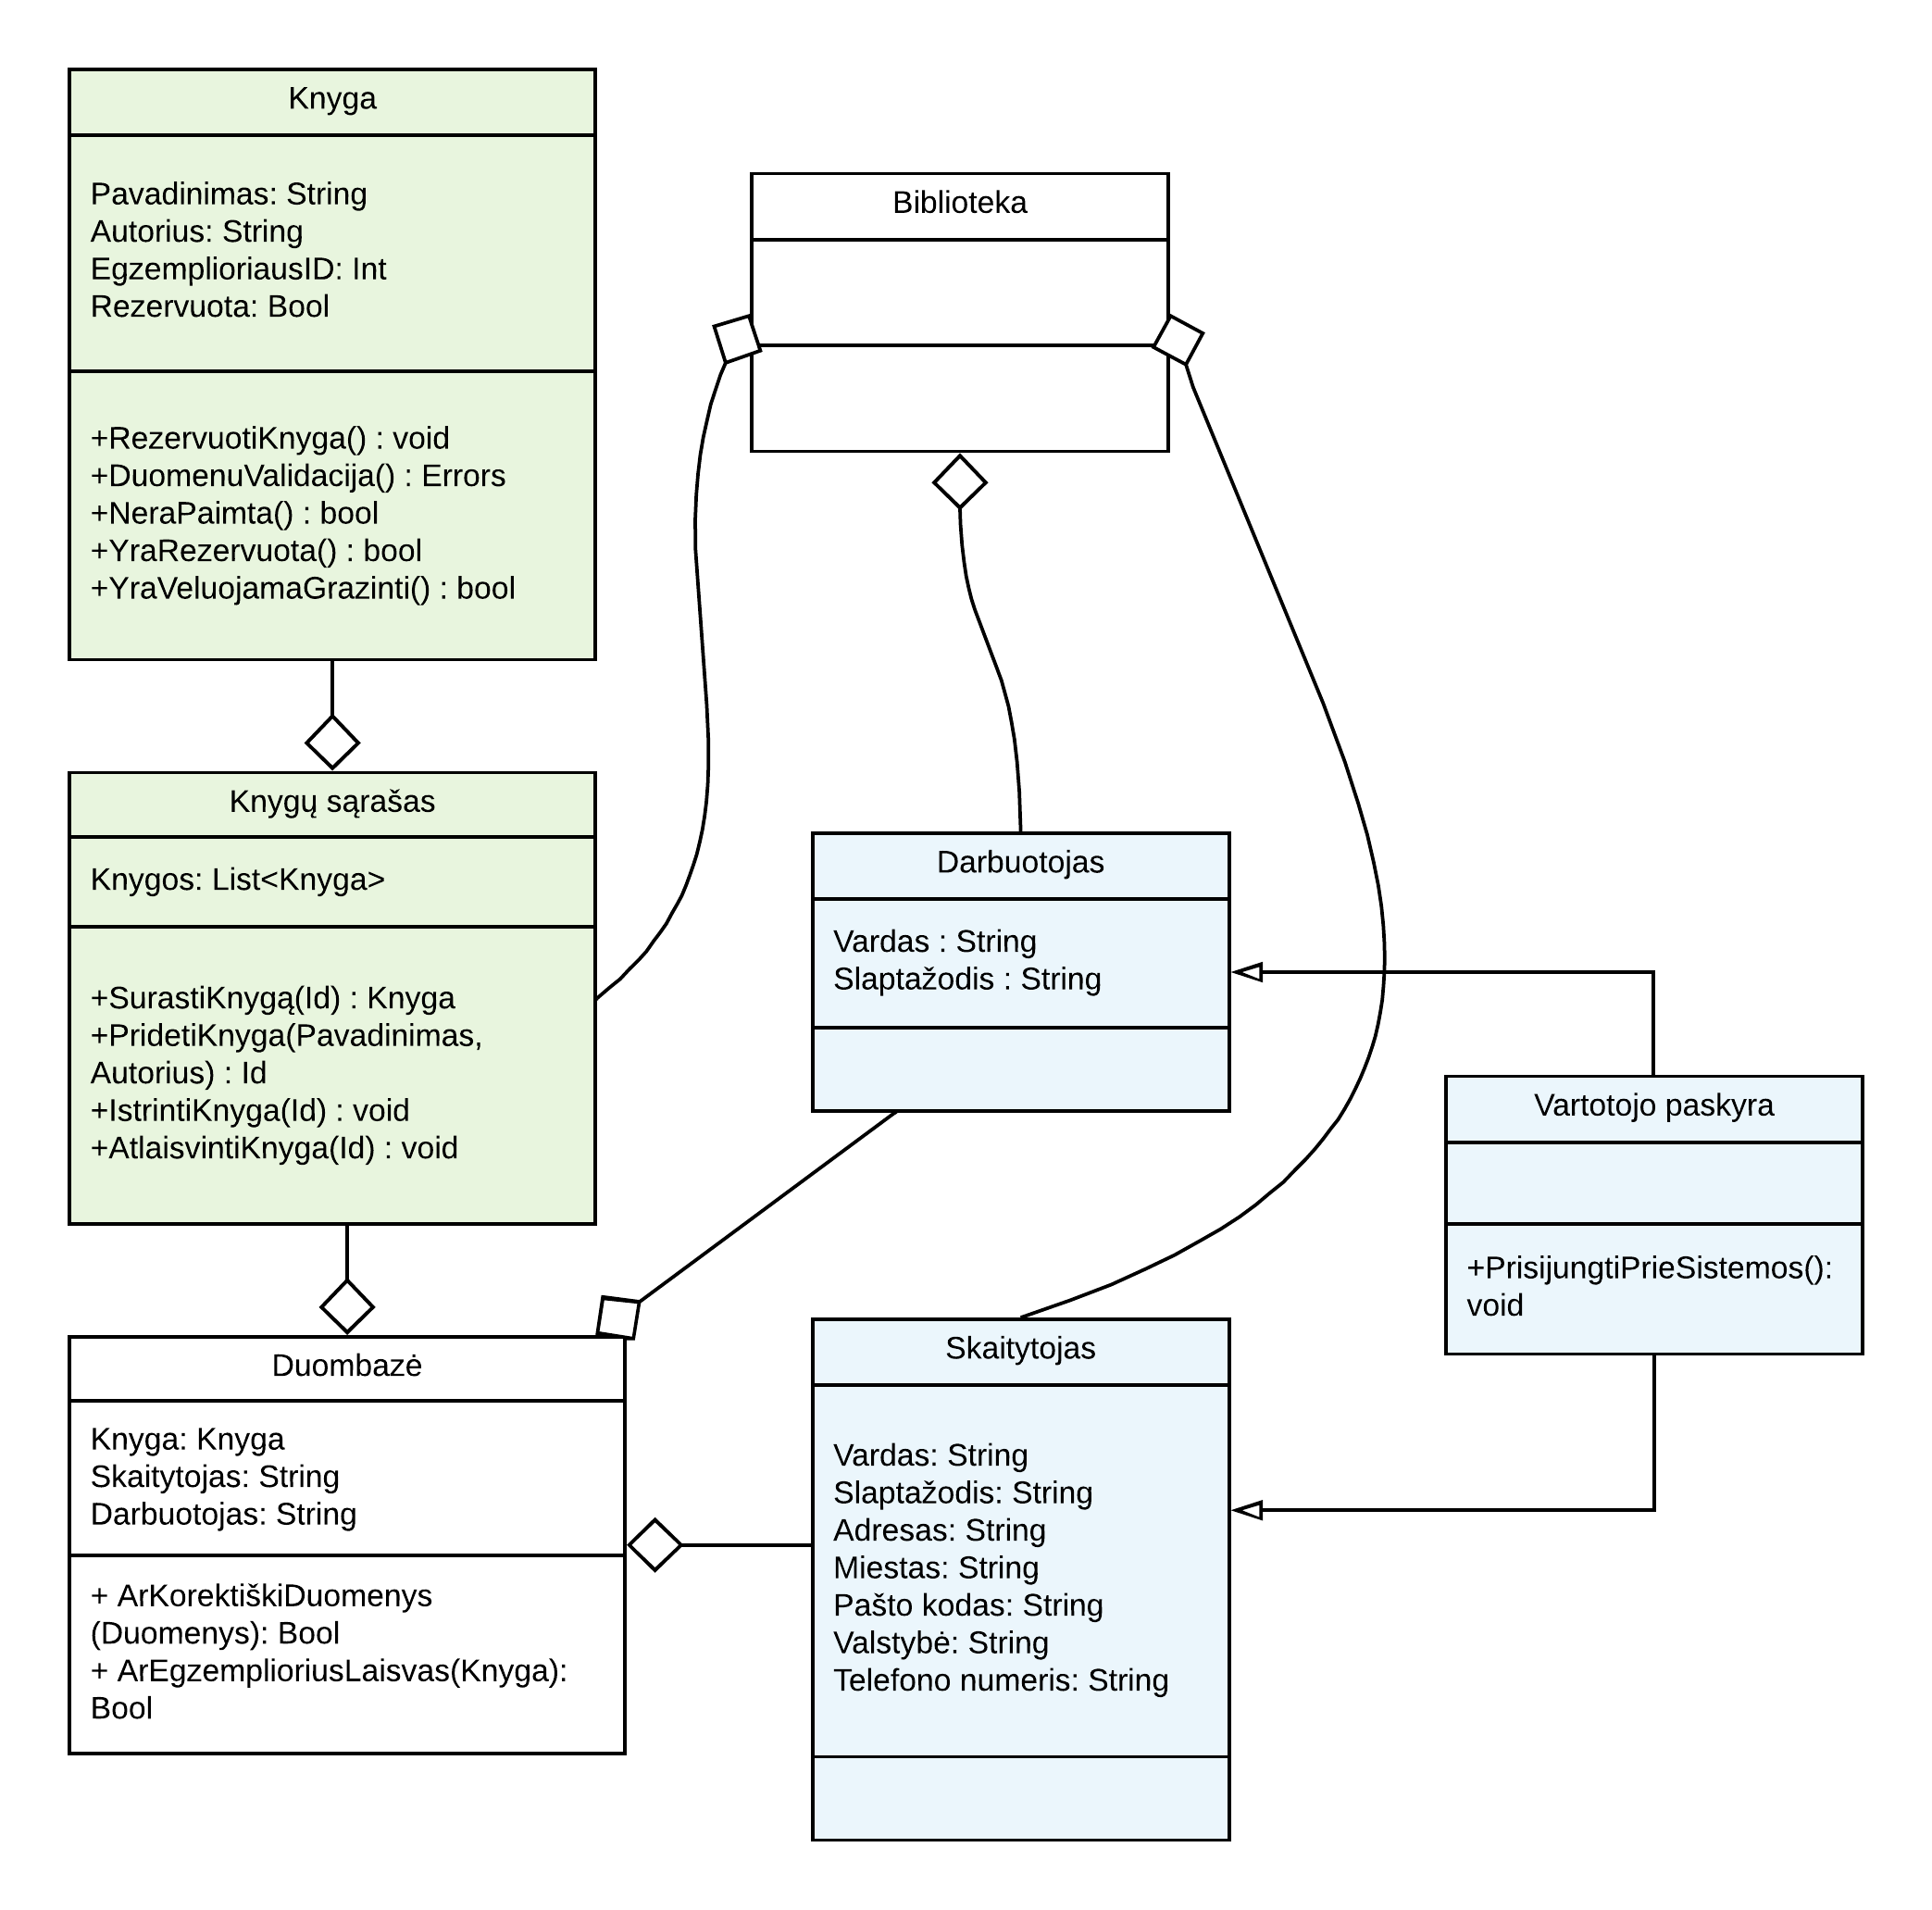
\includegraphics[width=1\textwidth]{diagramos/statinis_modelis.png}
    \caption{Struktūrinis dalykinės srities modelis} 
    
\end{figure}

Biblioteka yra pagrindinė esybė. Jai priklauso bibliotekos programėlės, darbuotojo, kliento ir knygos dalys. Šios esybės yra lemiamos. Nuo jų priklauso viso proceso veikimas. Darbuotojas aptarnauja skaitytojus, registruojant naujus klientus bei gali išimti bei pridėti knygas Bibliotekoje. Bibliotekos programėlė teikia informaciją apie knygų prieinamumą bei valdo knygų skolinimą ir grąžinimą. Skaitytojas sąveikauja su biblioteka, tai yra skolinasi ar grąžiną knygas, per bibliotekos programėlę.

\subsection{Struktūrinės dalykinės srities modelio matrica}

 Šiame poskyryje pateikiama reikalavimų - struktūrinio dalykinės srities modelio atsekamumo matrica. 

\begin{figure}[H]
    \centering
    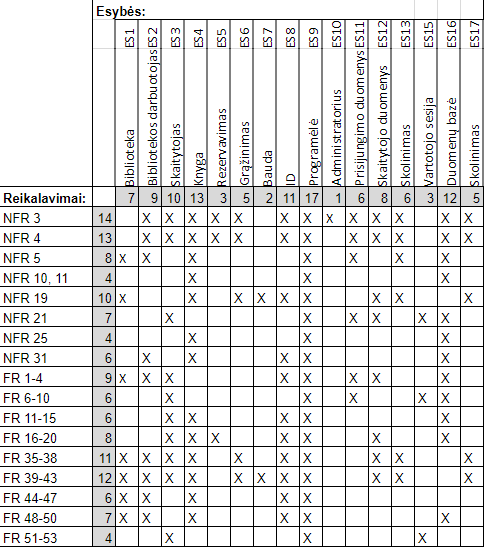
\includegraphics[width=1.05\textwidth]{matricos/matrreikesybes.png}
    \caption{Esybių ir reikalavimų matrica}    
\end{figure}


			\begin{comment}

\subsection{Dalykinės srities užduotys (tikslai)}

\begin{figure}[H]
    \centering
    \caption{Bibliotekos užduotys}
    \includegraphics[width=1\textwidth]{vidines/UC_Biblio_Uzduotys.png}
    
\end{figure}

Skaitytojas ir darbuotojas yra agentai kurie įgyvendina bibliotekoje esančias užduotis - užsiregistruoja, prisijungia, atlieka knygų paiešką, knygos skolinimasi, knygos grąžinimą. Atskirai darbuotojas atlieka  knygos pridėjimą, knygos išėmimą.\\
\indent
Darbuotojas aptarnauja skaitytoją, dėl to jis dalyvauja visose užduotyse.

\subsection{Dalykinės srities vykdymo scenarijai}

Šioje dalyje yra pateikiama didelė dalis visų galimų scenarijų, kurie gali nutikti bibliotekoje. Vartotojo registracija, prisijungimas, knygos paieška, knygos skolinimas, knygos grąžinimas.

\subsubsection{Vartotojo registracija bibliotekoje}

\begin{figure}[H]
    \centering
    \caption{Vartotojo registracija bibliotekoje}
    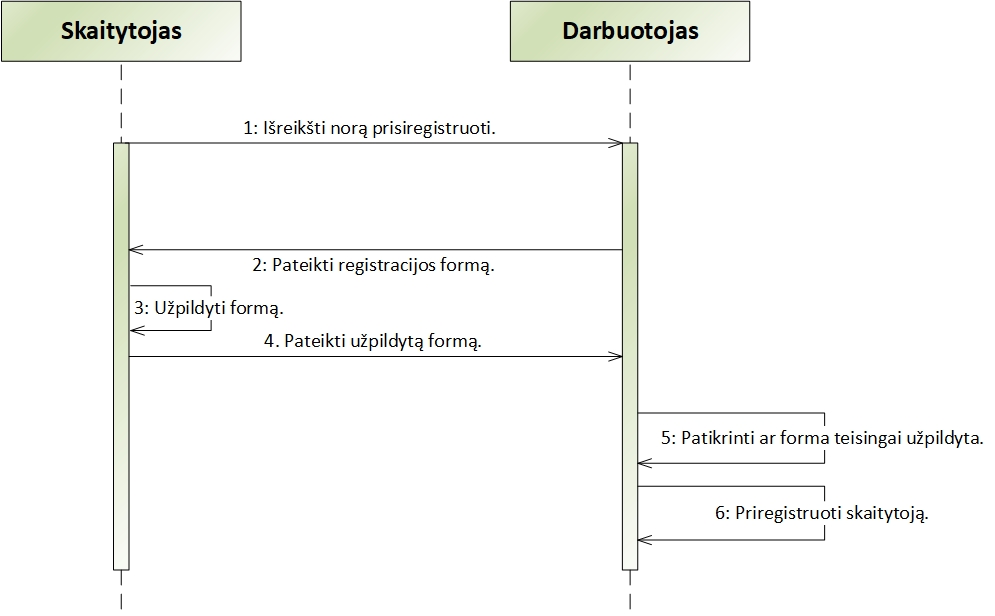
\includegraphics[width=1\textwidth]{vidines/SkaitytojoRegistracijosScenarijus}

\end{figure}

Skaitytojas norintis užsiregistruoti bibliotekoje turi joje apsilankyti. Gavęs iš darbuotojo registracijos formą turi ją atidžiai išpildyti. Kai skaitytojas grąžina išpildytą dokumentą, darbuotojas turi jį patikrinti. Jei nėra klaidų ir netrūksta jokių duomenų, darbuotojas priregistruoja naują skaitytoją.

\begin{figure}[H]
    \centering
    \caption{Vartotojo registracija bibliotekoje}
    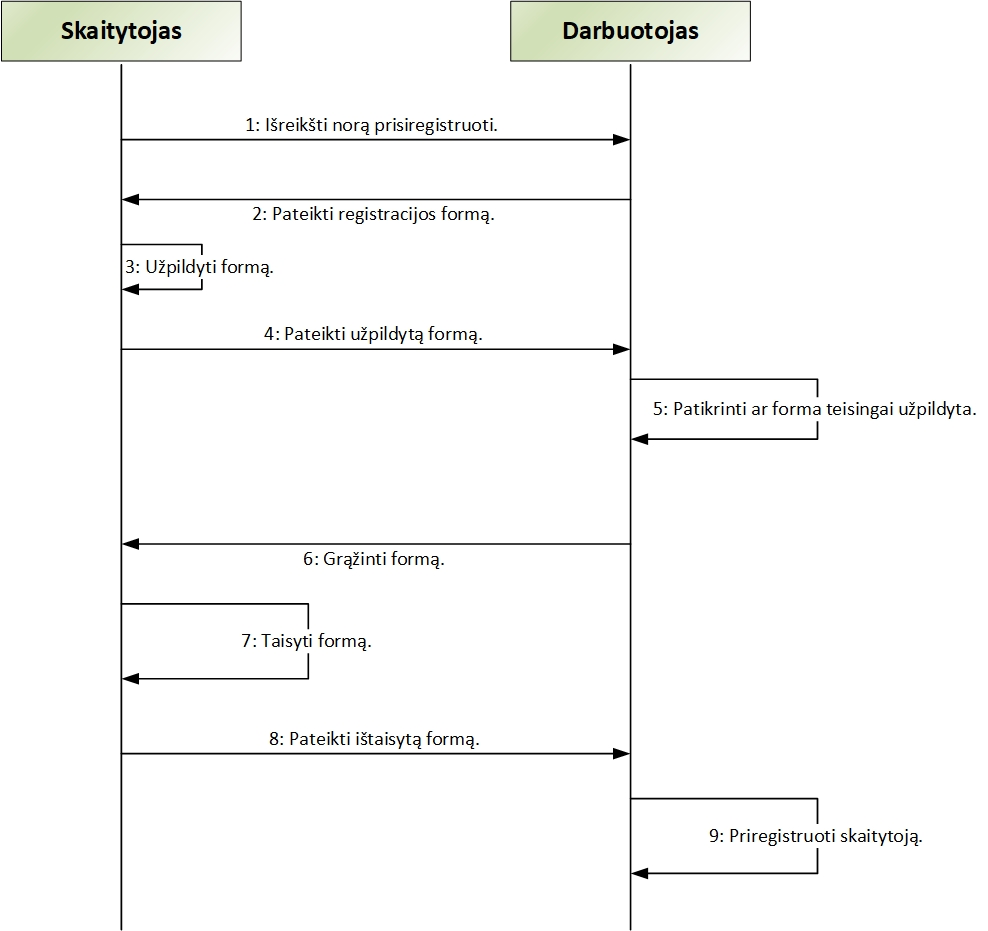
\includegraphics[width=1\textwidth]{vidines/SD_SkaitytojoRegistracija2}

\end{figure}

\indent
Jei atsiranda klaidų, ar trūksta duomenų darbuotojas grąžina formą skaitytojui. Kai dokumentas išpildytas taisyklingai, darbuotojas priregistruoja nauja skaitytoją prie bibliotekos.


\subsubsection{Vartotojo prisijungimas bibliotekoje}
\begin{figure}[H]
    \centering
    \caption{Vartotojo prisijungimas bibliotekoje}
    \includegraphics[width=1\textwidth]{vidines/SD_SkaitytojoPrisijungimas}

\end{figure}

Skaitytojas, norintis prisijungti į bibliotekos sistemą, turi suvęsti savo prisijungimo duomeis į el. bibliotekos sistemą.  Jei nėra prsijungimo klaidų ir skaistytojas yra duomenų bazėje, sistema prijungia skaitytoją prie sistemos. Sistema informuoja, kad skaitytojas yra sėkmingai prisijungęs ir leidžia naudotis bibliotekos teikiamomis paslaugomis.

\begin{figure}[H]
    \centering
    \caption{Vartotojo prisijungimas bibliotekoje}
    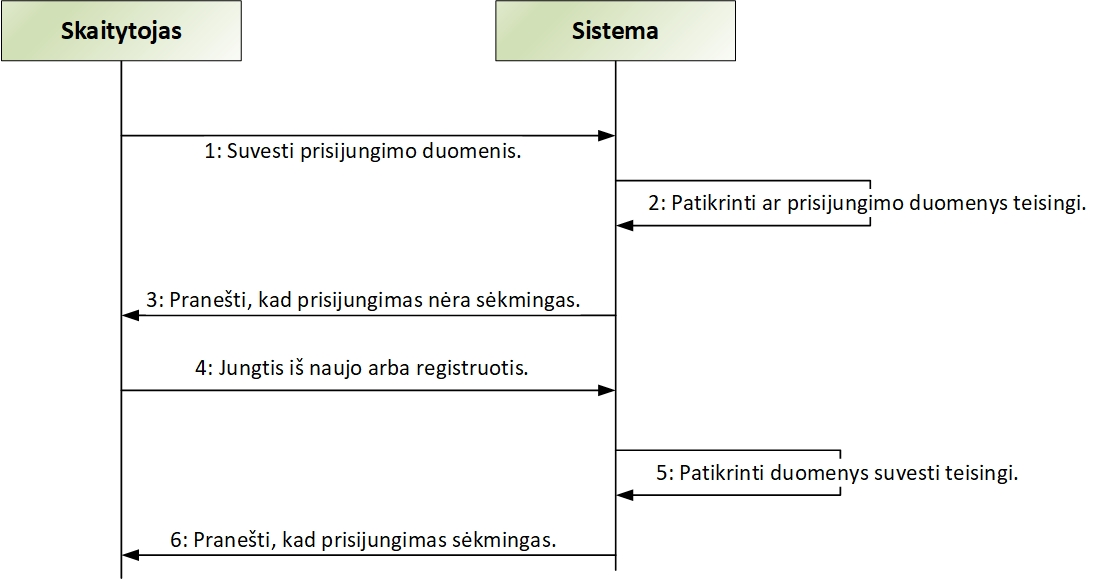
\includegraphics[width=1\textwidth]{vidines/SD_SkaitytojoPrisijungimas2}

\end{figure}

\indent
Jei atsiranda prisijungimo klaidų, ar trūksta duomenų apie skaitytoją duomenų bazėjesistema įspėja apie tai skaitytoją. Skaitytojas bando jungti prie sistemos dar kartą, arba registruotis. Kai skaitytojo duomenys išpildyti taisyklingai, sistema prijungia skaitytoją prie bibliotekos.


\subsubsection{Knygos paieška}

\begin{figure}[H]
    \centering
    \caption{Knygos paieška}
    \label{fig:pa}
    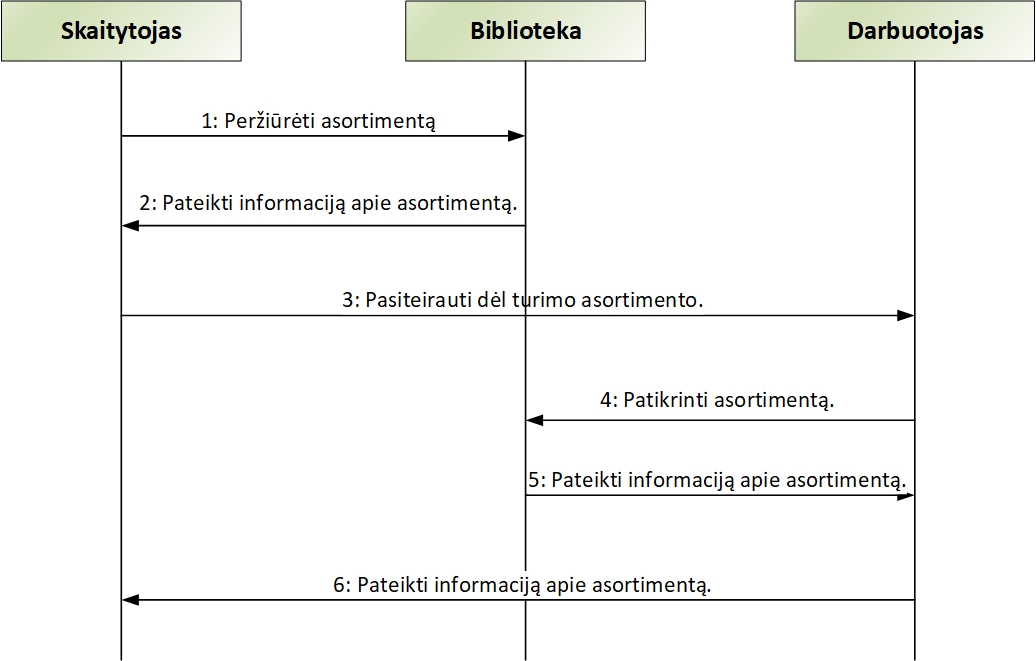
\includegraphics[width=1\textwidth]{vidines/SD_KnygosPaieska}

\end{figure}

Skaitytojas norėdamas susipažinti su bibliotekos asortimentu gali peržiūrėti jos lentynas. Dažnai tokia paieška nebūna sekminga. Skaitytojas norėdamas įsitikinti, kad norimos knygos nėra bibliotekoje turi paklausti darbuotojo. Jis, turint priegą prie skolinimų istorijos, gali suteikti informaciją apie asortimento prieinamumą.

\subsubsection{Knygos skolinimas}

\begin{figure}[H]
    \centering
    \caption{Knygos skolinimas}
    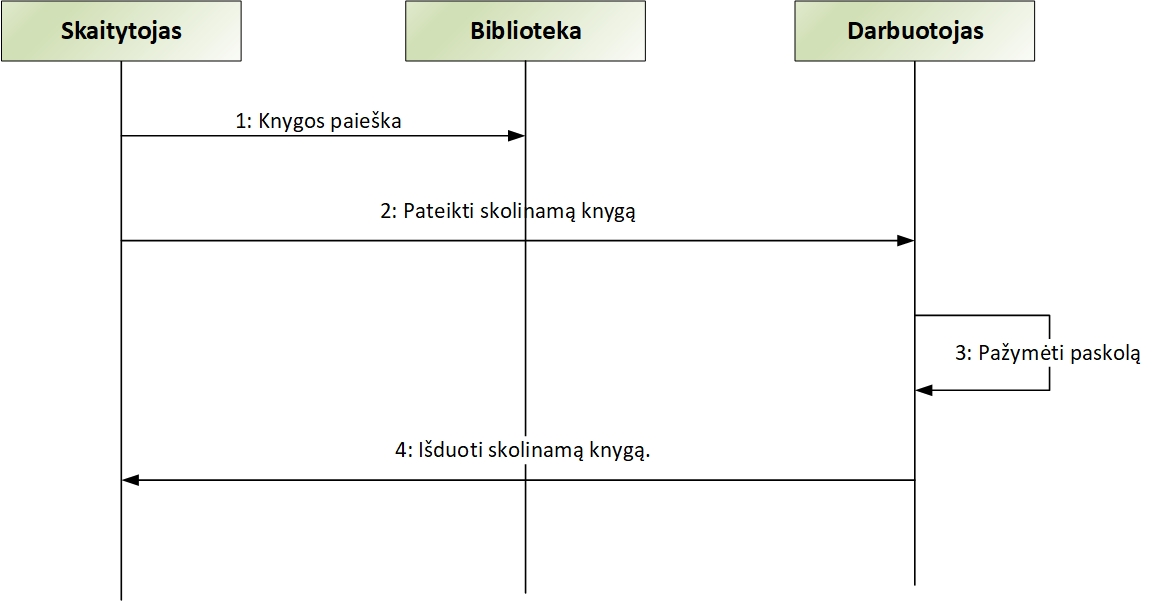
\includegraphics[width=1\textwidth]{vidines/SD_KnygosSkolinimas}

\end{figure}

Skaitytojas norintis pasiskolinti knygą iš pradžių turi atlikti jos paieška nurodyta \ref{fig:pa} diagramoje. Suradęs ieškomą knygą, skaitytojas apie tai praneša darbuotojui. Šis užrašo pasiskolinimą ir atiduoda knygą skaitytojui.

\subsubsection{Knygos grąžinimas}

\begin{figure}[H]
    \centering
    \caption{Knygos grąžinimas}
    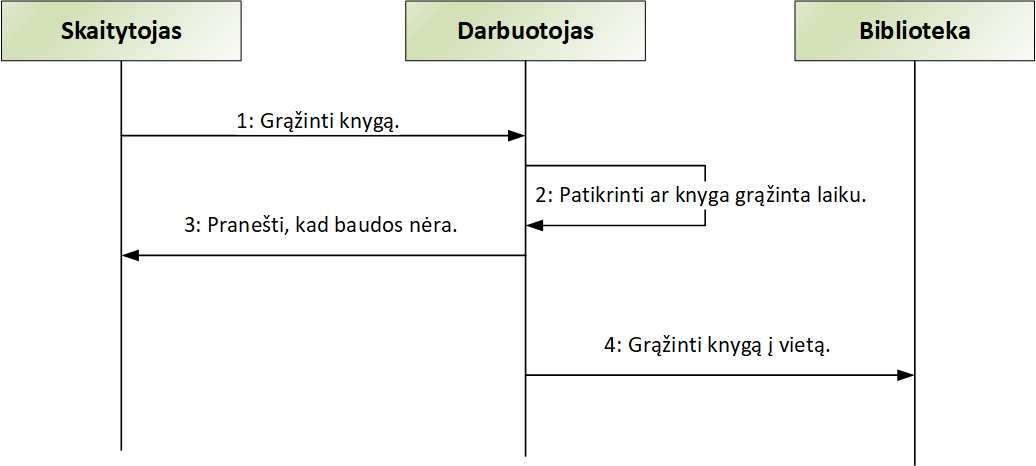
\includegraphics[width=1\textwidth]{vidines/SD_KnygosGra_inimas}

\end{figure}

Skaitytojas norintis grąžinti knygą turi ją pateikti darbuotojui. Jis patikrina, ar skola gražinta laiku. Jei bauda nepriskaičiuojama - knyga sėkmingai gražinta.

\begin{figure}[H]
    \centering
    \caption{Knygos grąžinimas}
    \includegraphics[width=1\textwidth]{vidines/SD_KnygosGra_inimas2}

\end{figure}

\indent
Kai skola grąžinama po termino, darbuotojas pranešia apie baudos dydį. Tada skaitytojas privalo ją sumokėti.


\subsection{Dalykinės srities dinaminė struktūra}
\subsubsection{Skaitytojo būsenos}

\begin{figure}[H]
    \centering
    \caption{Skaitytojo būsenos}
    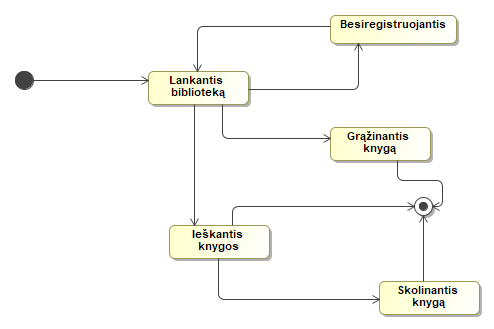
\includegraphics[width=1\textwidth]{vidines/stm__Skaitytojas__Skaitytojas}

\end{figure}

Skaitytojas priima būseną "Lankantis biblioteką" kai į ją ižengia. Jei apsilanko pirmą kartą, turi užsiregistruoti. Priima "Besiregistruojančio" būseną. Kai sėkmingai užsiregistruoja, gali atlikti knygos paieška. Šiuo ateveju būsena pasikeičia į "Ieškantis knygos". Kai skaitytojas suranda norima knygą pradėda ją skolinti. Tampa "Skolinančiu knygą". Skaitytojas norintis grąžinti knygą iš būsenos "Besilankantis bibliotekoje" tampa "Grąžinantis knygą".

\subsubsection{Darbuotojo būsenos}

\begin{figure}[H]
    \centering
    \caption{Darbuotojo būsenos}
    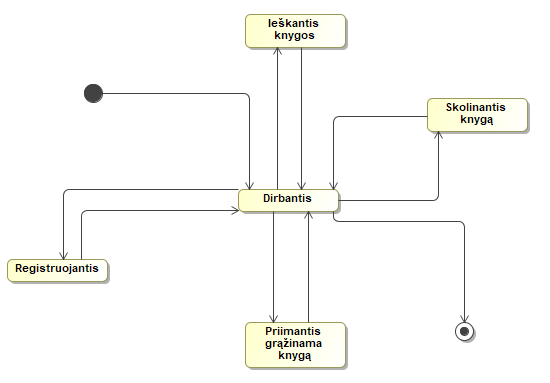
\includegraphics[width=1\textwidth]{vidines/stm__Darbuotojas__Darbuotojas}

\end{figure}

Darbuotojo pradinė būsena yra "Dirbantis". Priklausomai nuo skaitytojo poreikio, jis gali priimti viena iš keturių būsenų. Kai reikia užregistruoti nauja skaitytoją, darbuotojas tampa "Registruojančiu". Jei skaitytojui ieškant knygos prireikia pagalbos, darbuotojas priima būsena "Ieškantis knygos". Skaitytojui apsisprendus dėl norimos knygos jis pradėda ją skolinti. Šiuo atveju darbuotojas tampa "Skolinančiu knygą". Kai knyga yra grąžinama, darbuotojas priima būseną "Priimantis grąžinama knygą".


				\end{comment}

\section{Programos langų sąrašas}
Šiame skyriuje pateiktas visų programos langų sąrašas (neskaitant pranešimo ar klaidos langų):
	\begin{itemize}
    \item Registracijos langas
    \item Prisijungimo langas
    \item Bibliotekos pagrindinis langas
    \item Vartotojo meniu
    \item Knygos grąžinimo langas
    \item Knygos pridėjimo langas
    \item Knygos ištrinimo langas
\item Knygos duomenų langas 
    
    \end{itemize}

\section{Užduotys}

Šiame skyriuje pateikiami sistemos atliekamų užduočių pagrindiniai ir alternatyvūs scenarijai. Sekų diagramose alternatyvieji scenarijai yra pažymėti raudona spalva.

\subsection{Vartotojo užduotys}

Šiame poskyryje yra pateikiami vartotojo atliekami užduočių pagrindiniai ir alternatyvūs scenarijai (žr. \ref{fig:ucVart}).

\begin{figure}[H]

\label{fig:ucVart}
    \centering
    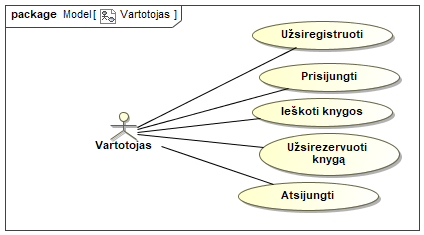
\includegraphics[width=1\textwidth]{vidines/ucVart}
    \caption{Vartotojo užduočių diagrama}

\end{figure}

\pagebreak

\subsubsection{Užsiregistravimas U1}

\begin{comment}
\begin{figure}[H]
\caption{Vartotojo registravimo sekų diagrama}
\label{fig:sdVart}
    \centering
    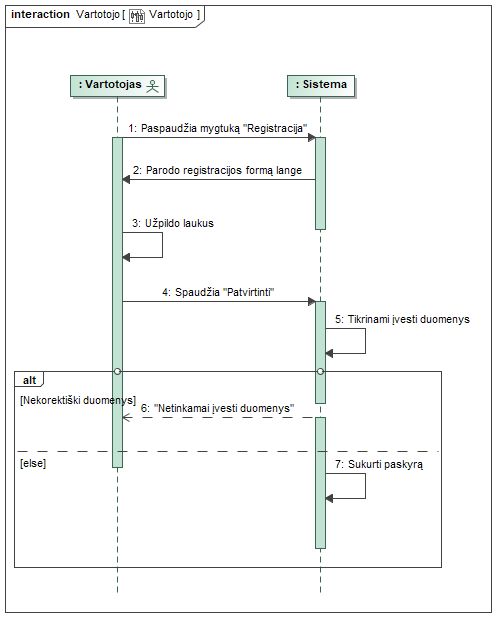
\includegraphics[width=1\textwidth]{vidines/sdVartotojo}

\end{figure}
\end{comment}

	\textbf{Tikslas:} Vartotojui sukurti paskyrą (žr. 4 pav.).
    
	\textbf{Pagrindinis scenarijus :} Neužsiregistravęs vartotojas pradiniame lange paspaudžia mygtuką "Registracija".Sistema parodo registracijos langą, kuriame yra laukai: vardas, slaptažodis, adresas, miestas, pašto kodasvalstybė, papildoma informacija ir telefono numeris. Korektiškai užpildžius laukus (dėl laukų korektiškumo žiūrėti FR.1.),vartotojas spaudžia "Patvirtinti" ir yra sukuriama vartotojui jo paskyra.

	\textbf{Alternatyvūs scenarijai }
    	\begin{enumerate}
    	\item Jeigu vartotojas įveda netinkamus duomenis arba toks vartotojo vardas
			  jau užregistruotas, išvedama informacija apie netinkamą duomenų įvedimą.
        \item Jei vartotojas nepatvirtina registracijos negalės buti užregistruotas.
        
    	\end{enumerate}

	\textbf{Nuoroda į reikalavimus:} FR.1.- FR.4.

\begin{figure}[H]
\label{fig:regdiag}
    \centering
    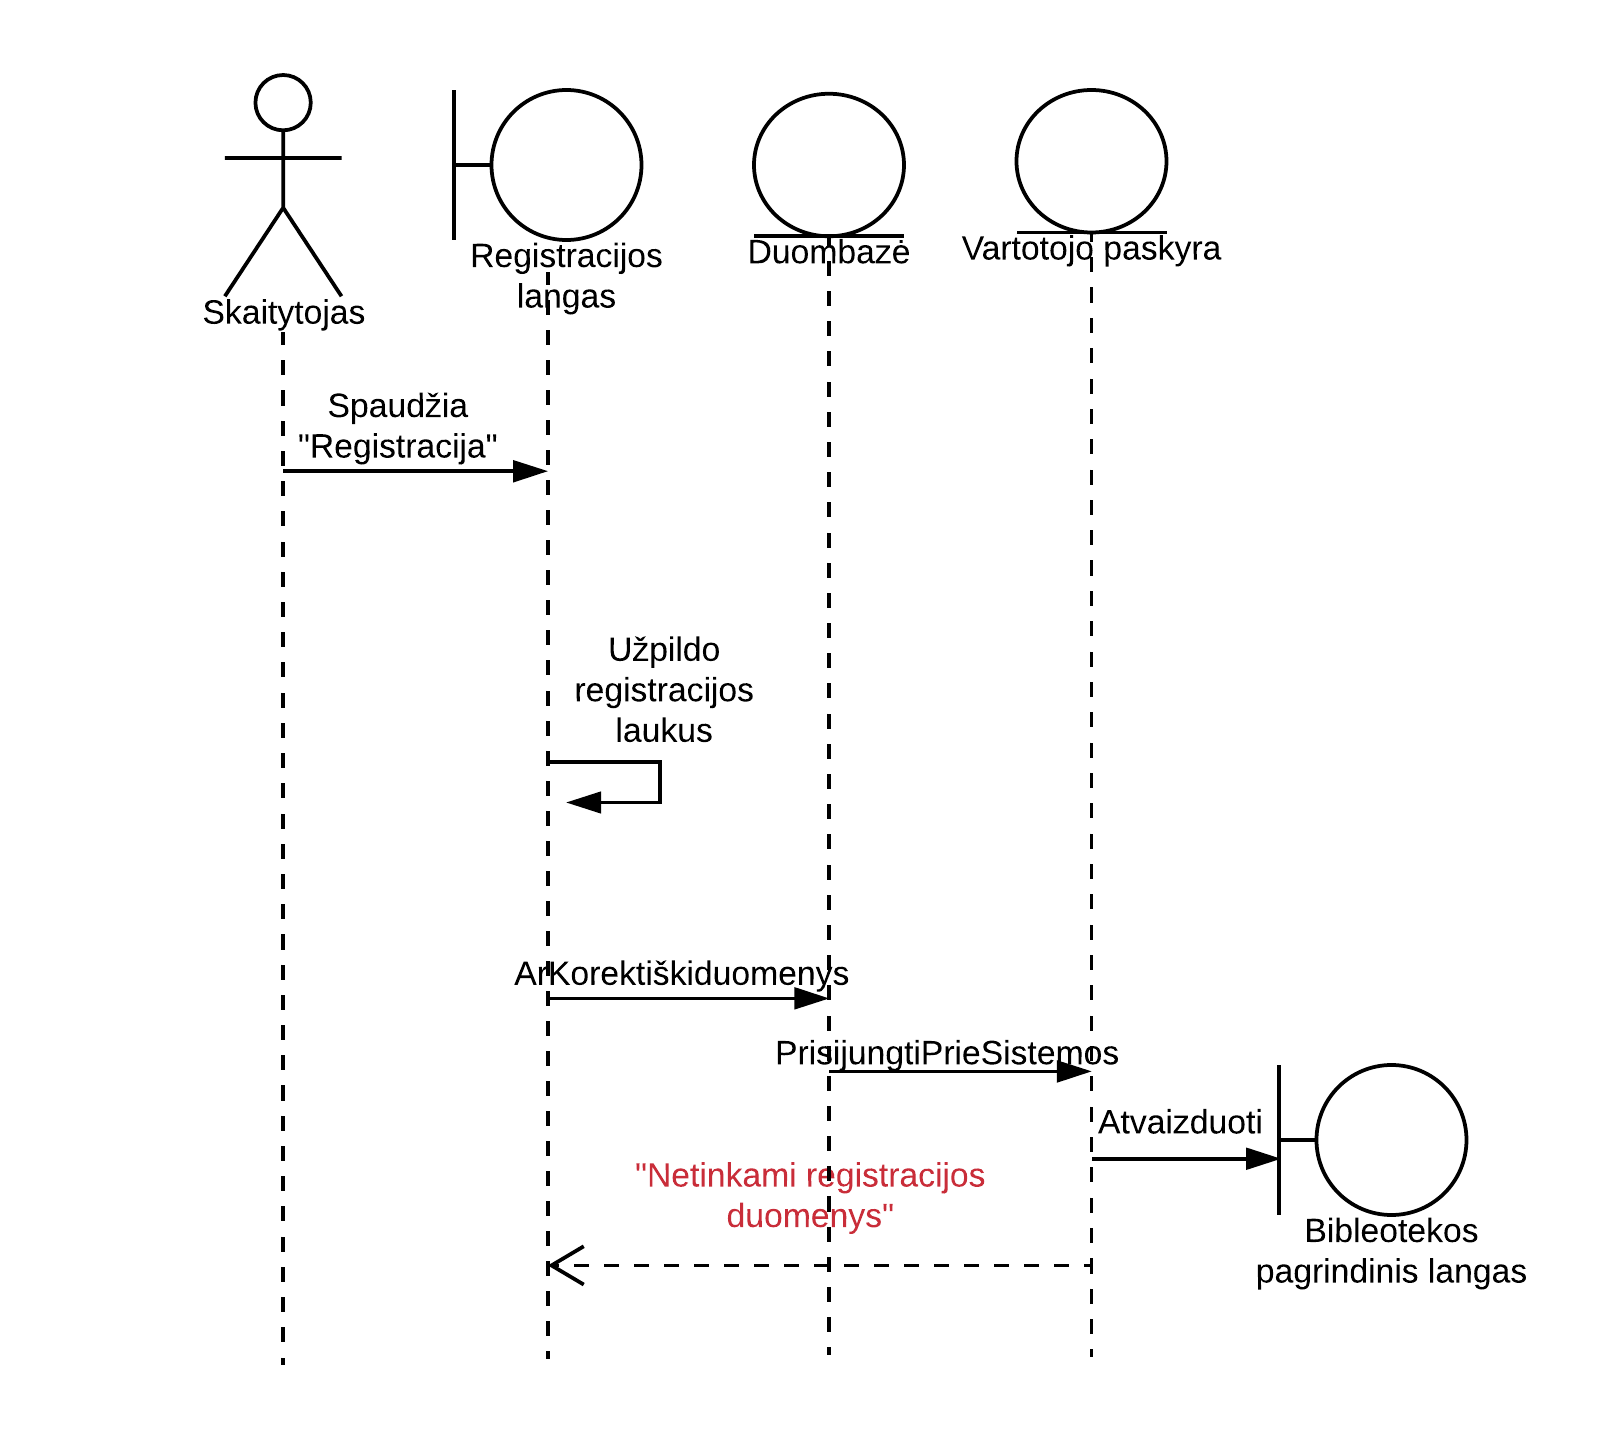
\includegraphics[width=1\textwidth]{Sekos_diagramos/SD_Registracija}
	\caption{registracijos diagrama}  
\end{figure}

\subsubsection{Prisijungimas U2} 

\begin{comment}

\begin{figure}[H]
\caption{Vartotojo registravimo sekų diagrama}
\label{fig:sdPris}
    \centering
    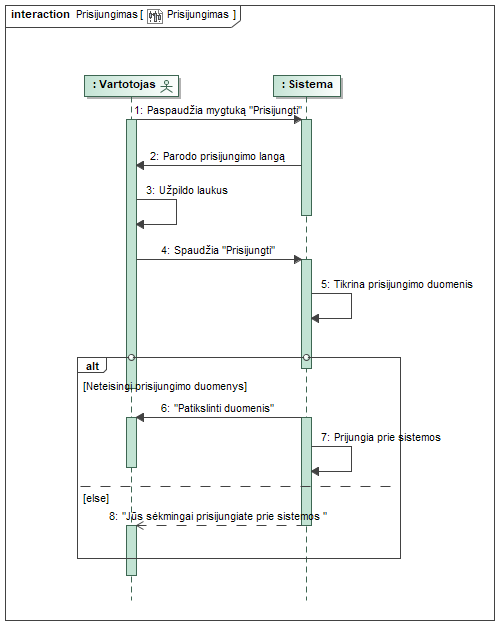
\includegraphics[width=0.7\textwidth]{vidines/sdPrisijungimas}

\end{figure}

\end{comment}

\begin{figure}[H]
\label{fig:prslang}
    \centering
    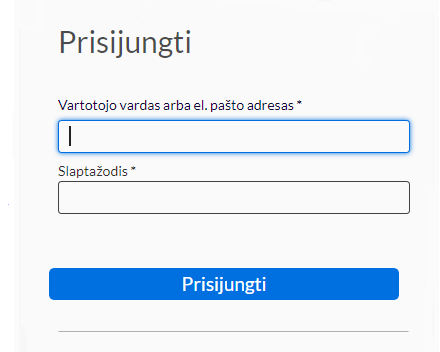
\includegraphics[width=0.7\textwidth]{vidines/ucprisijungti}
	\caption{prisijungimo langas}
\end{figure}

	\textbf{Tikslas:} Vartotojui (arba darbuotojui) prisijungti prie programos (žr. 6 pav.) .

	\textbf{Pagrindinis scenarijus :} Vartotojas bibleotekos prisijungimo lange paspaudžia mygtuką "Prisijungti".
Sistema parodo prisijungumo langą (žr. 5 pav.), kuriame yra laukai: vardas,slaptažodis, prisijungimo tipas (žr. FR. 6.1.). Vartotojas įveda prisijungimo duomenis, pasirenka prisijungimo tipą, patvirtina prisijungimą ir spaudžia mygtuką "Prisijungti". Sistema patikrina prisijungimo duomenis, jei teisingai įvesti, prijungia vartotoją prie sistemos ir jam praneša apie sėkmingą prisijungimą.

	\textbf{Alternatyvūs scenarijai :} 
    	\begin{enumerate}
			\item Neteisingai įvedus duomenis arba nieko neįvedus išvedama informacija dėl duomenų 	   	 	  					patikslinimo.
		\end{enumerate} 


	\textbf{Nuoroda į reikalavimus: FR.6. - FR.10.}
    
\begin{figure}[H]
\label{fig:logindiag}
    \centering
    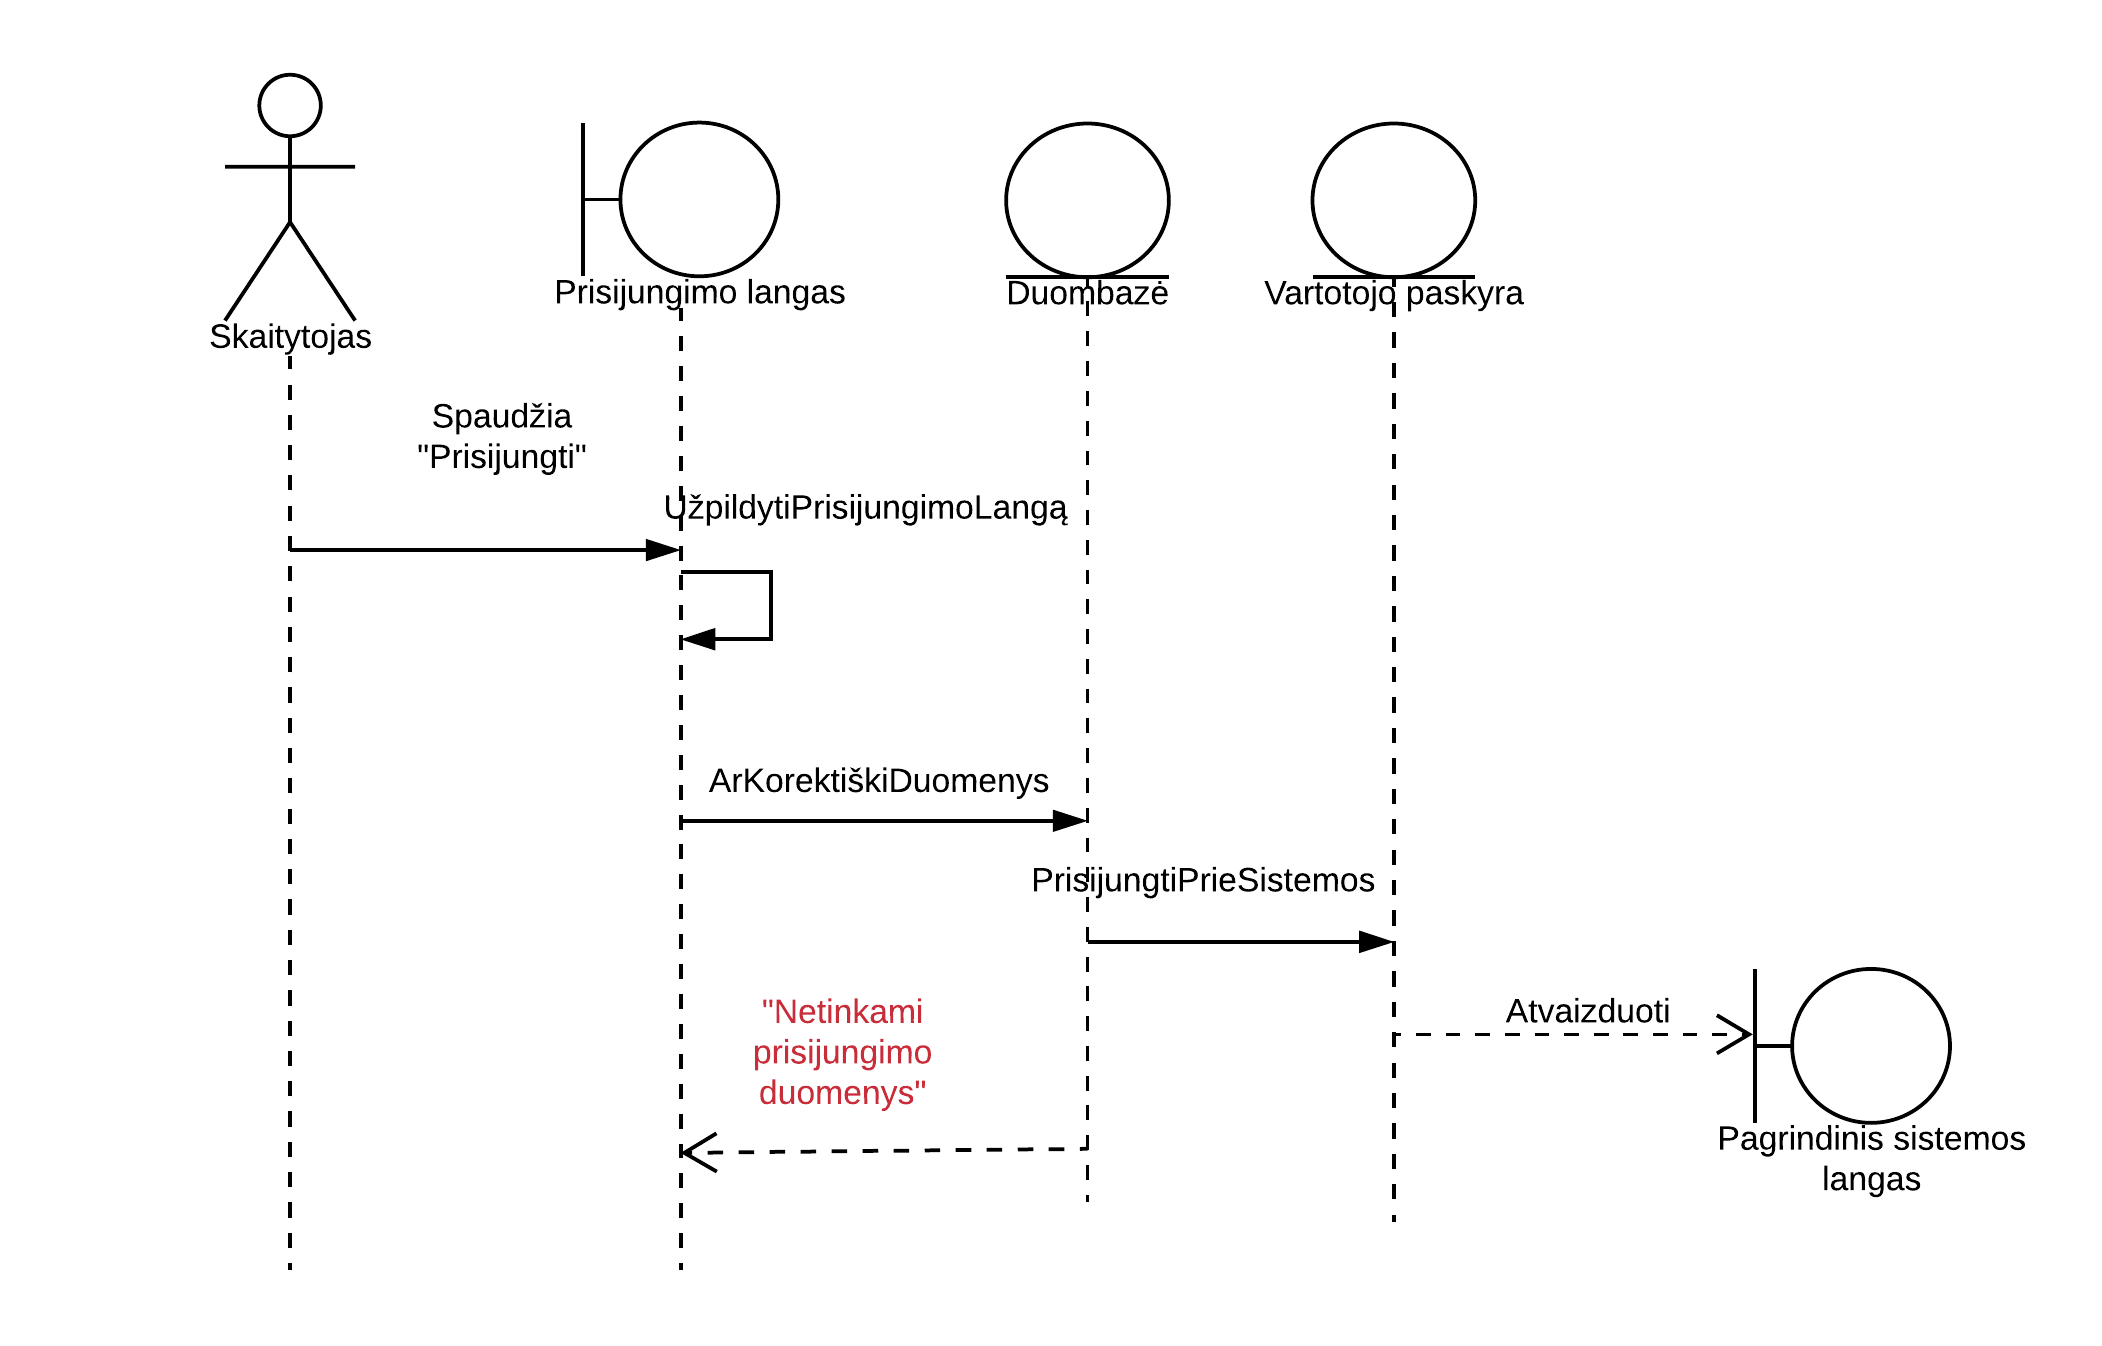
\includegraphics[width=1\textwidth]{Sekos_diagramos/SD_Prisijungimas}   
	\caption{Prisijungimo diagrama}
\end{figure}

 \subsubsection{Knygos ieškojimas U3}


\begin{figure}[H]
\label{fig:knylang}
    \centering
    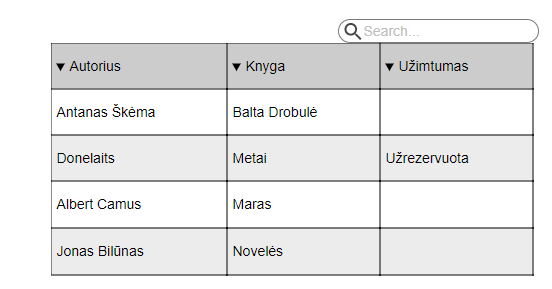
\includegraphics[width=1\textwidth]{vidines/ucpaieska}
	\caption{Knygos paieškos langas}
\end{figure}

	\textbf{Tikslas:} Surasti ieškomą knygą (žr. 8 pav.).

	\textbf{Pagrindinis scenarijus :}Vartotojas įveda knygos pavadinimo arba autoriaus vardo ar pavardės dalį į paieškos langelį (žr. \ref{fig:knylang}). Sistema vykdo knygos paiešką ir gražina knygų sąrašą pagal įvestą žodį ar žodžio dalį jį parodo pagrindiniame lange.

	\textbf{Alternatyvūs scenarijai :}
    \begin{enumerate}
    \item Jeigu vartotojas nieko neįvedė į paieškos langą, tai Sistema grąžina visą bibliotekoje esančių knygų 		     sąrašą, kurį parodo pagrindiniame lange.
    \item Jeigu sistema neranda vartotojo ieškomos knygos, grąžinamas tuščias sąrašas.
    \end{enumerate}


	\textbf{Nuoroda į reikalavimus:} FR.11. - FR.15.
    
\begin{figure}[H]
\label{fig:searchdiag}
    \centering
    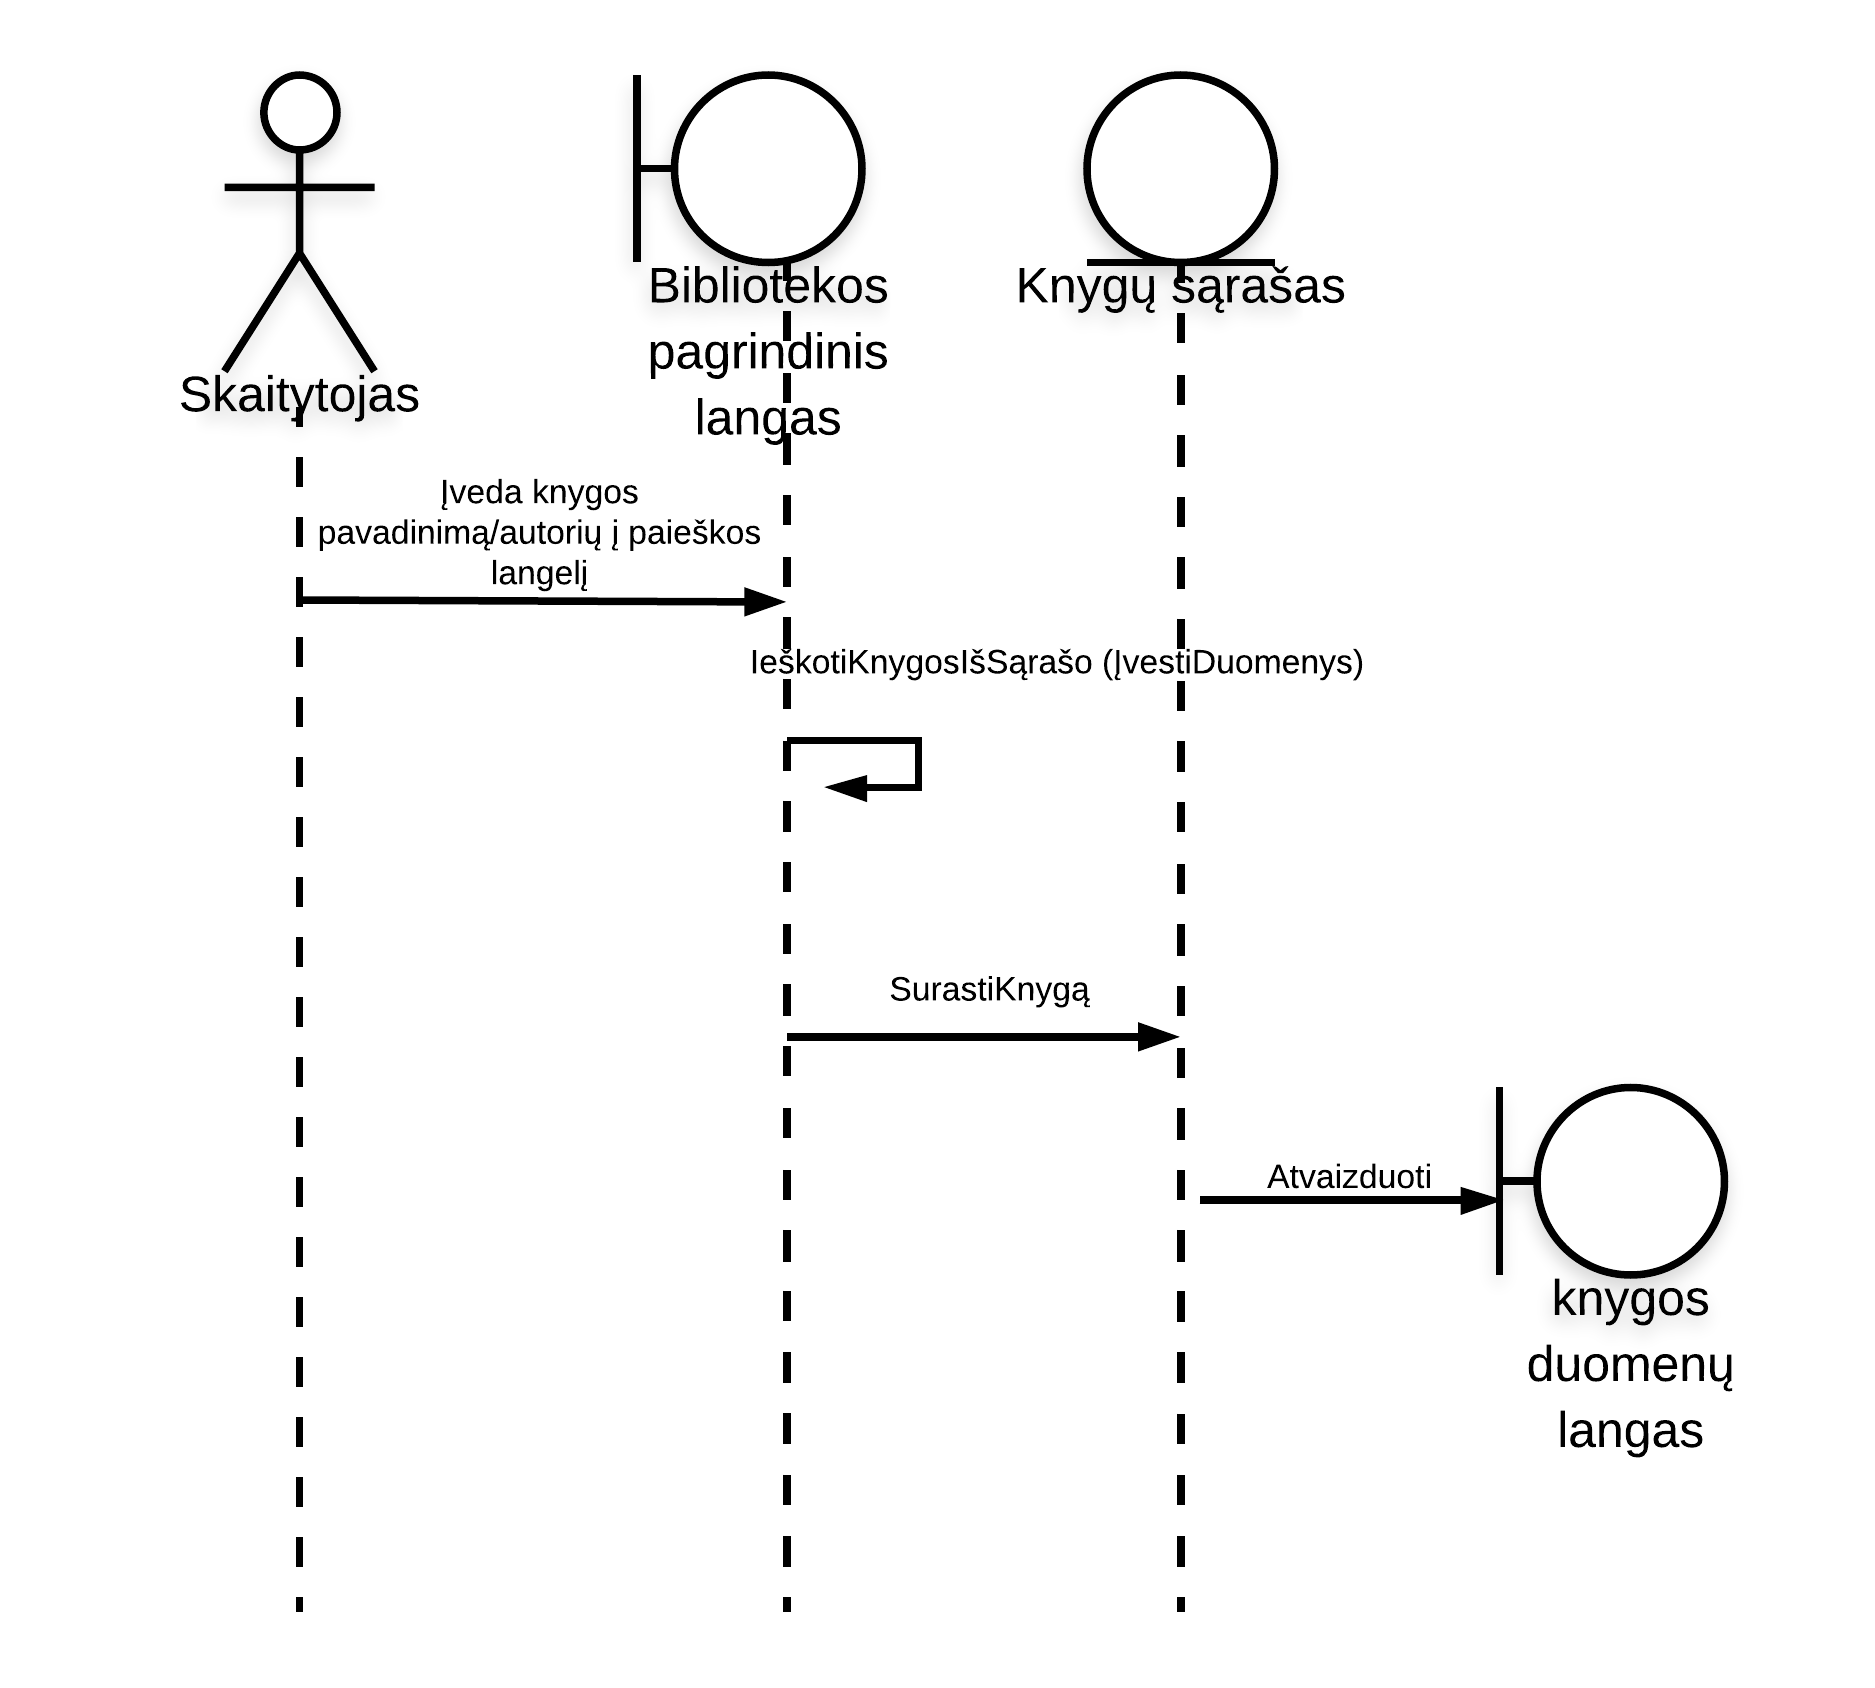
\includegraphics[width=1\textwidth]{Sekos_diagramos/SD_Paieska}
	\caption{paieškos diagrama}
\end{figure}

\subsubsection{Knygos rezervavimas U4}

\begin{comment}

\begin{figure}[H]
\caption{Knygos rezervavimo sekų diagrama}
\label{fig:Reserve}
    \centering
    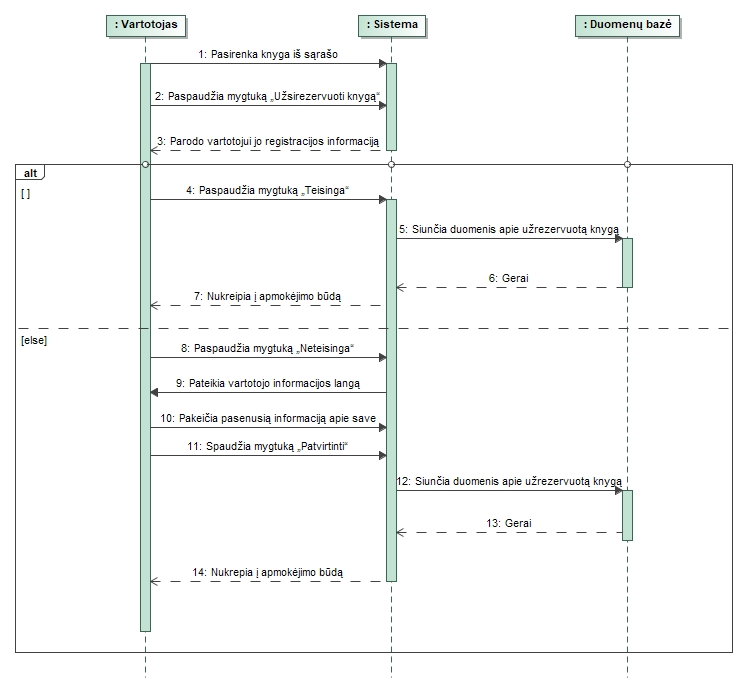
\includegraphics[width=0.7\textwidth]{diagramos/Reserve}

\end{figure}

\end{comment}

	\textbf{Tikslas:} Rezervuoti knygą.

	\textbf{Pagrindinis scenarijus :} Sistema pateikia vartotojui laisvų knygų sąrašą, esantį sistemoje. Vartotojas pasirenką norimą knygą ir paspaudžia mygtuką „Užsirezervuoti knygą“. Sistema parodo vartotojui jo pasirinkimą, šios knygos egzempliorio numerį ir prašo patvirtinti jį. Tada jis paspaudžia mygtuką „Taip“, patvirtindamas savo pasirinkimą. Sistema siunčia užklausą į duomenų bazę, kuri papildoma naujos rezervacijos duomenimis.
    
	\textbf{Alternatyvūs scenarijai :} Jeigu šiuo metu nėra laisvo, norimos knygos, egzempliorio, skaitytojui apie tai yra pranešama ir pateikiama informacija, kada būtų galima tikėtis gauti knygą. Po to vartotojas yra nukreipiamas į knygos rezervacijos langą.

	\textbf{Nuoroda į reikalavimus:} FR.16.-FR.20.
    
\begin{figure}[H]
\label{fig:rezervdiag}
    \centering
    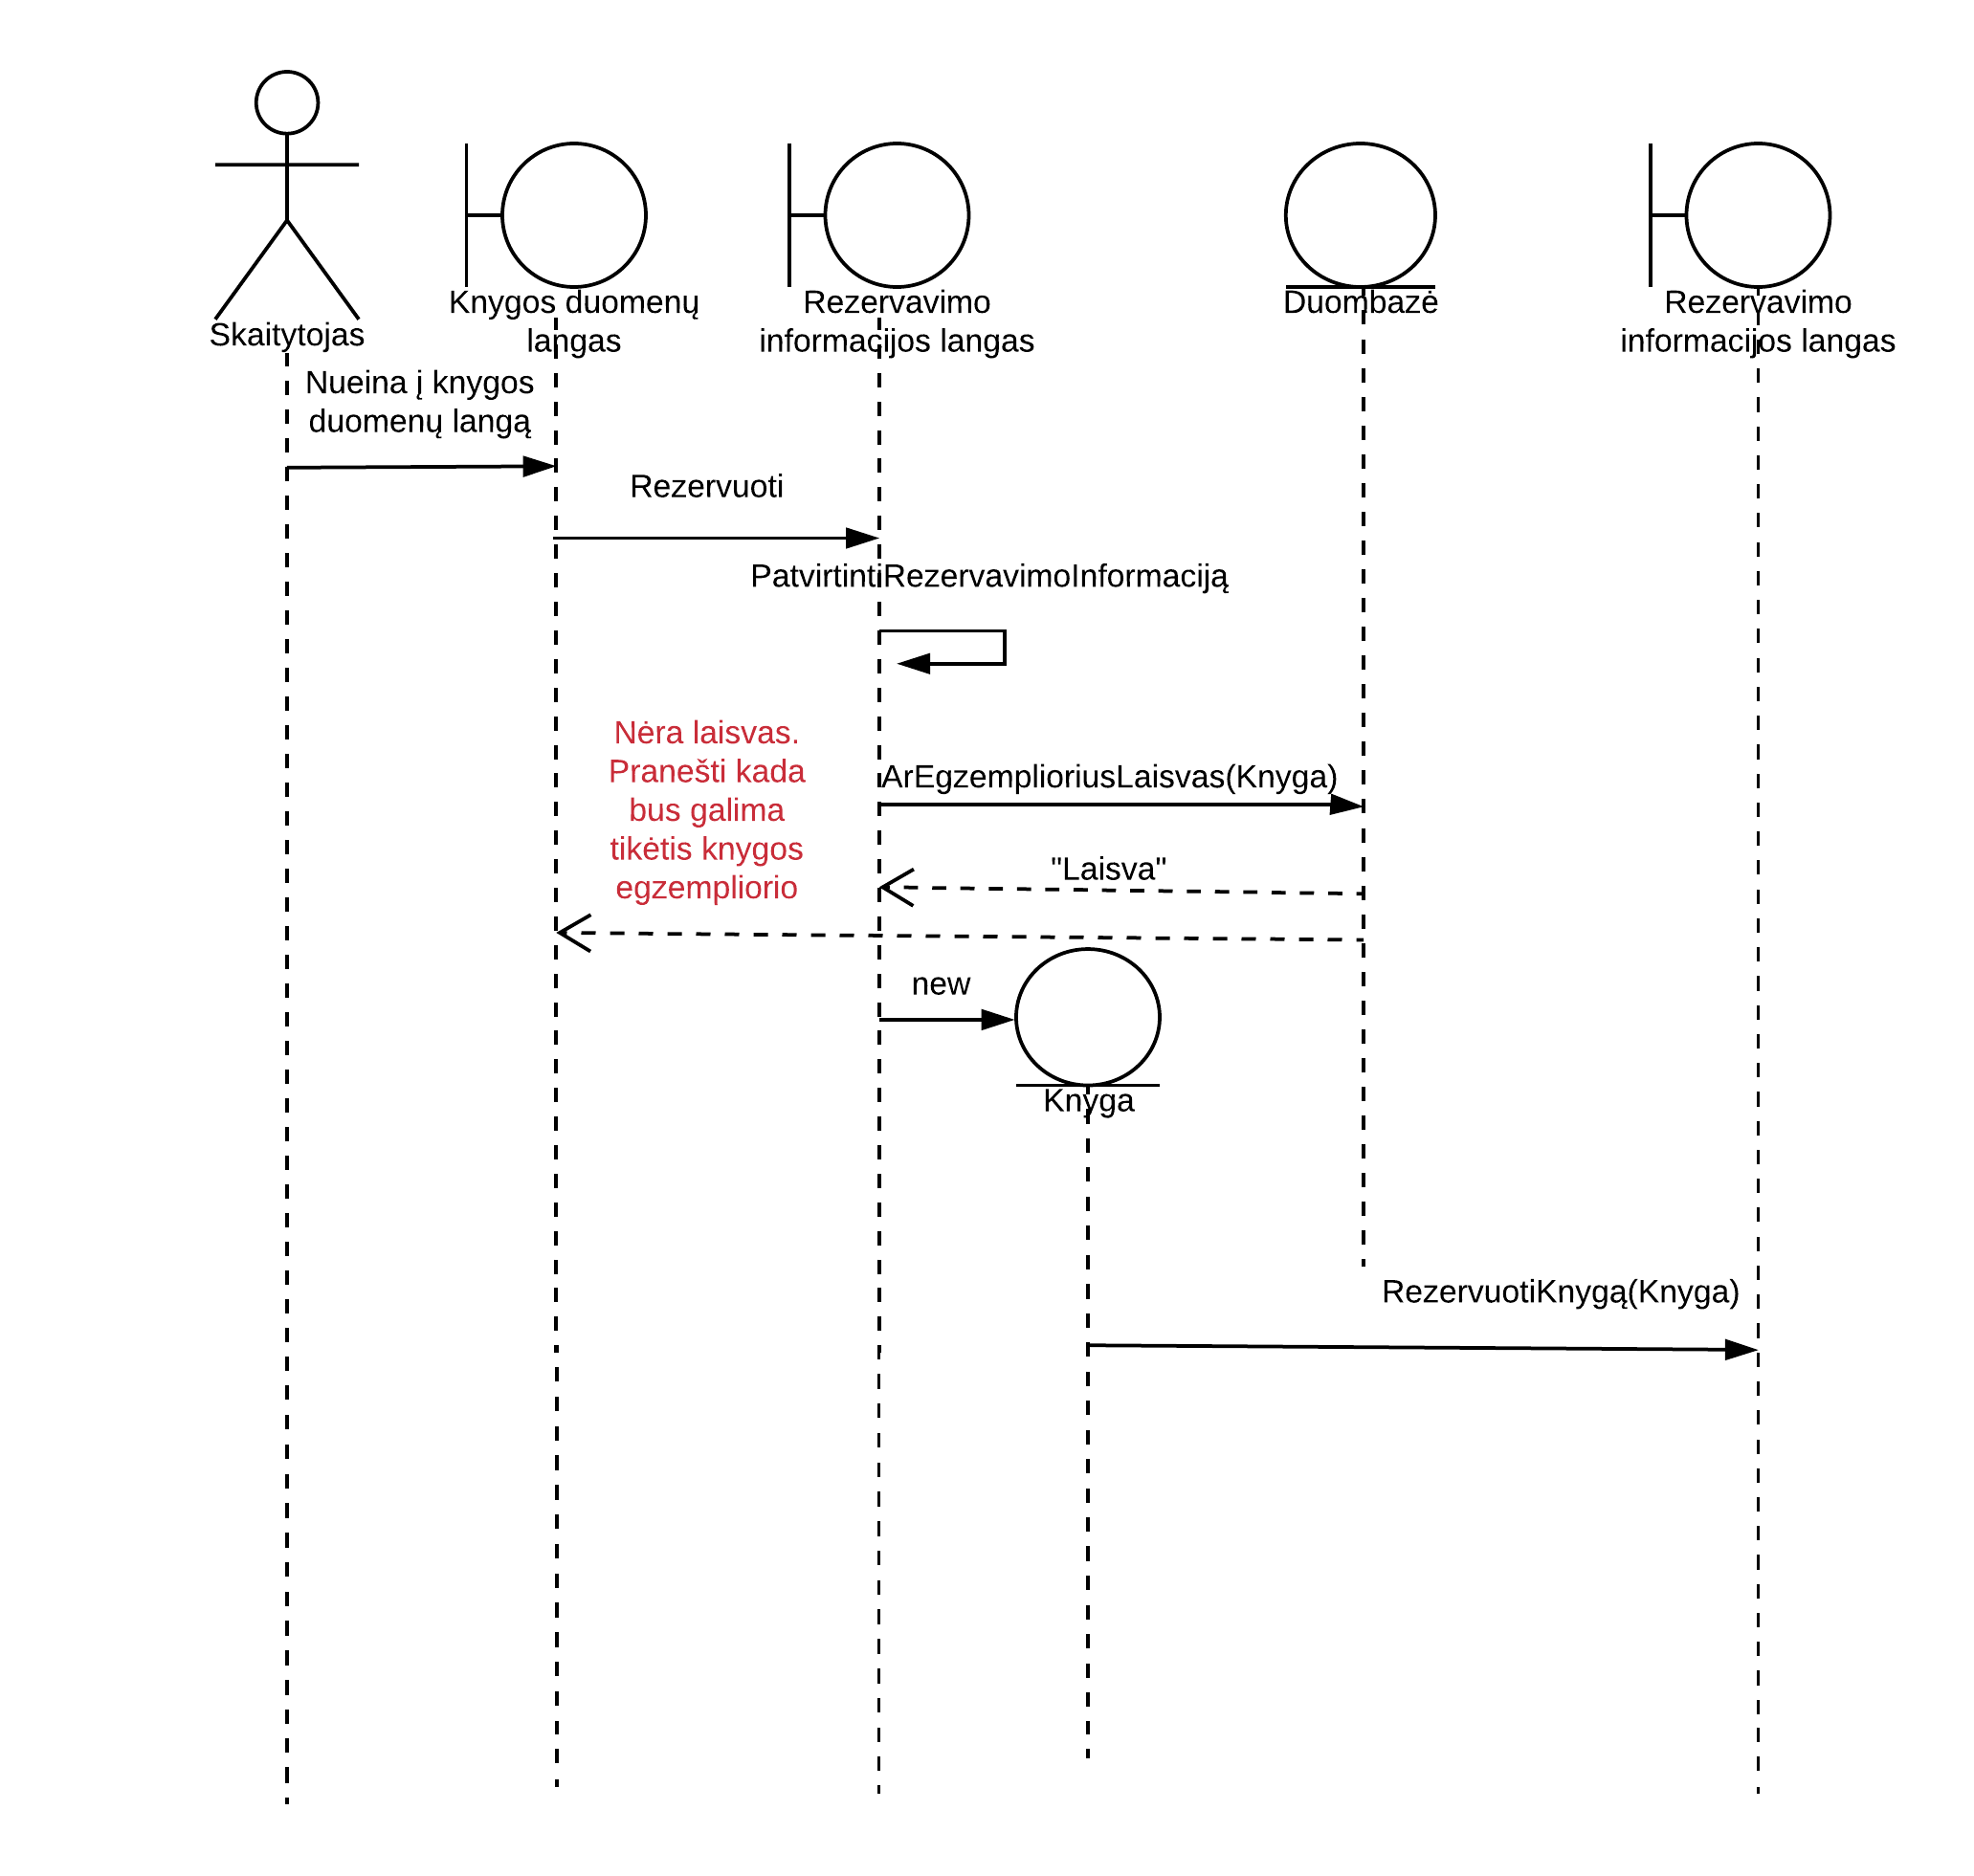
\includegraphics[width=1\textwidth]{Sekos_diagramos/SD_KRezervacija}
	\caption{rezervacijos diagrama}
\end{figure}

\begin{comment}
    
\subsubsection{Knygos grąžinimo termino pratęsimas U5}

\begin{figure}[H]
\caption{Vartotojo ir darbuotojo ryšis norint prasitęsti terminą}
\label{fig:ucVartDarb}
    \centering
    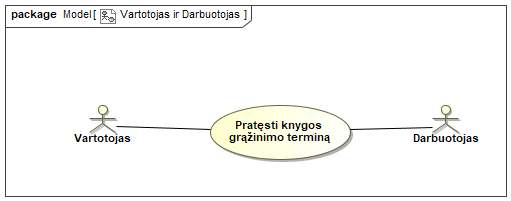
\includegraphics[width=0.7\textwidth]{vidines/ucVartDarb}
    
Aukščiau pavaidzuotoje diagramoje (žr. \ref{fig:ucVartDarb}) norima parodyti, jog tik darbuotojas turi teisę pratęsti knygos grąžinimo terminą. Vartotojas pateikia darbuotojui knygos informaciją, kurią nori pratęsti.

\end{figure}

\begin{figure}[H]
\caption{Knygos grąžinimo termino pratęsimo sekų diagrama}
\label{fig:Continue}
    \centering
    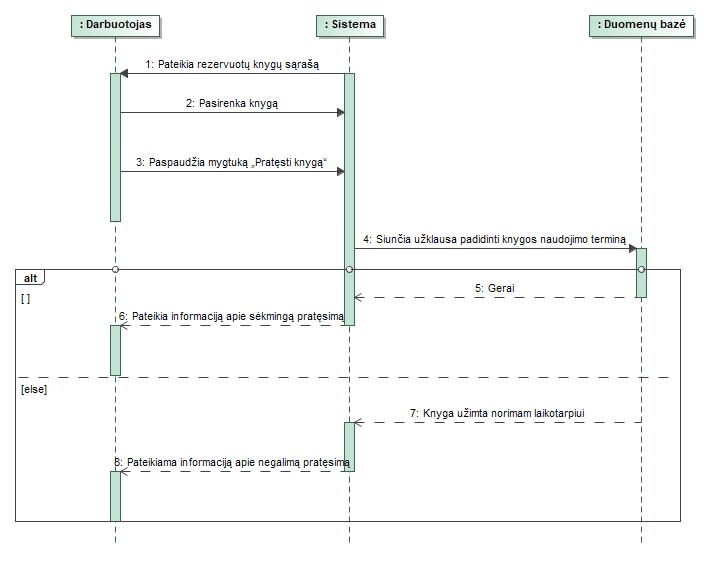
\includegraphics[width=0.7\textwidth]{diagramos/Continue}

\end{figure}

	\textbf{Tikslas:} Pratęsti knygos grąžinimo terminą.

	\textbf{Pagrindinis scenarijus :} Sistema pateikia darbuotojui vartotojo rezervuotų knygų sąrašą ir darbuotojas pasirenka norimą pratęsti knygą paspausdamas mygtuką „Pratęsti knygą“. Tada sistema siunčia užklausą į duomenų bazę, kur padidinamas knygos grąžinimo terminas  vienu mėnesiu. Darbuotojui pateikiama informaciją apie sėkmingą termino pratęsimą.

	\textbf{Alternatyvūs scenarijai :} Jeigu knyga duomenų bazėje jau yra užimta norimam pratęsimo laikotarpiui, tada duomenų bazė nepapildoma, o darbuotojui pateikiama informaciją apie negalimą pratęsimą nurodytam terminui.

	\textbf{Nuoroda į reikalavimus:} FR.31.-FR.34.
    \end{comment}

 \subsubsection{Atsijungimas U6}

	\textbf{Tikslas:} Atsijungti nuo sistemos.

	\textbf{Pagrindinis scenarijus:} Vartotojas paspaudžia mygtuką ”Atsijungti” ir atsijungia nuo sistemos.

	\textbf{Alternatyvūs scenarijai:} Išjungus programą vartotojas yra automatiškai atjungiamos nuo sistemos.

	\textbf{Nuoroda į reikalavimus:} FR.51. - FR.53.
    
\begin{figure}[H]
    \label{fig:logoffdiag}
    \centering
    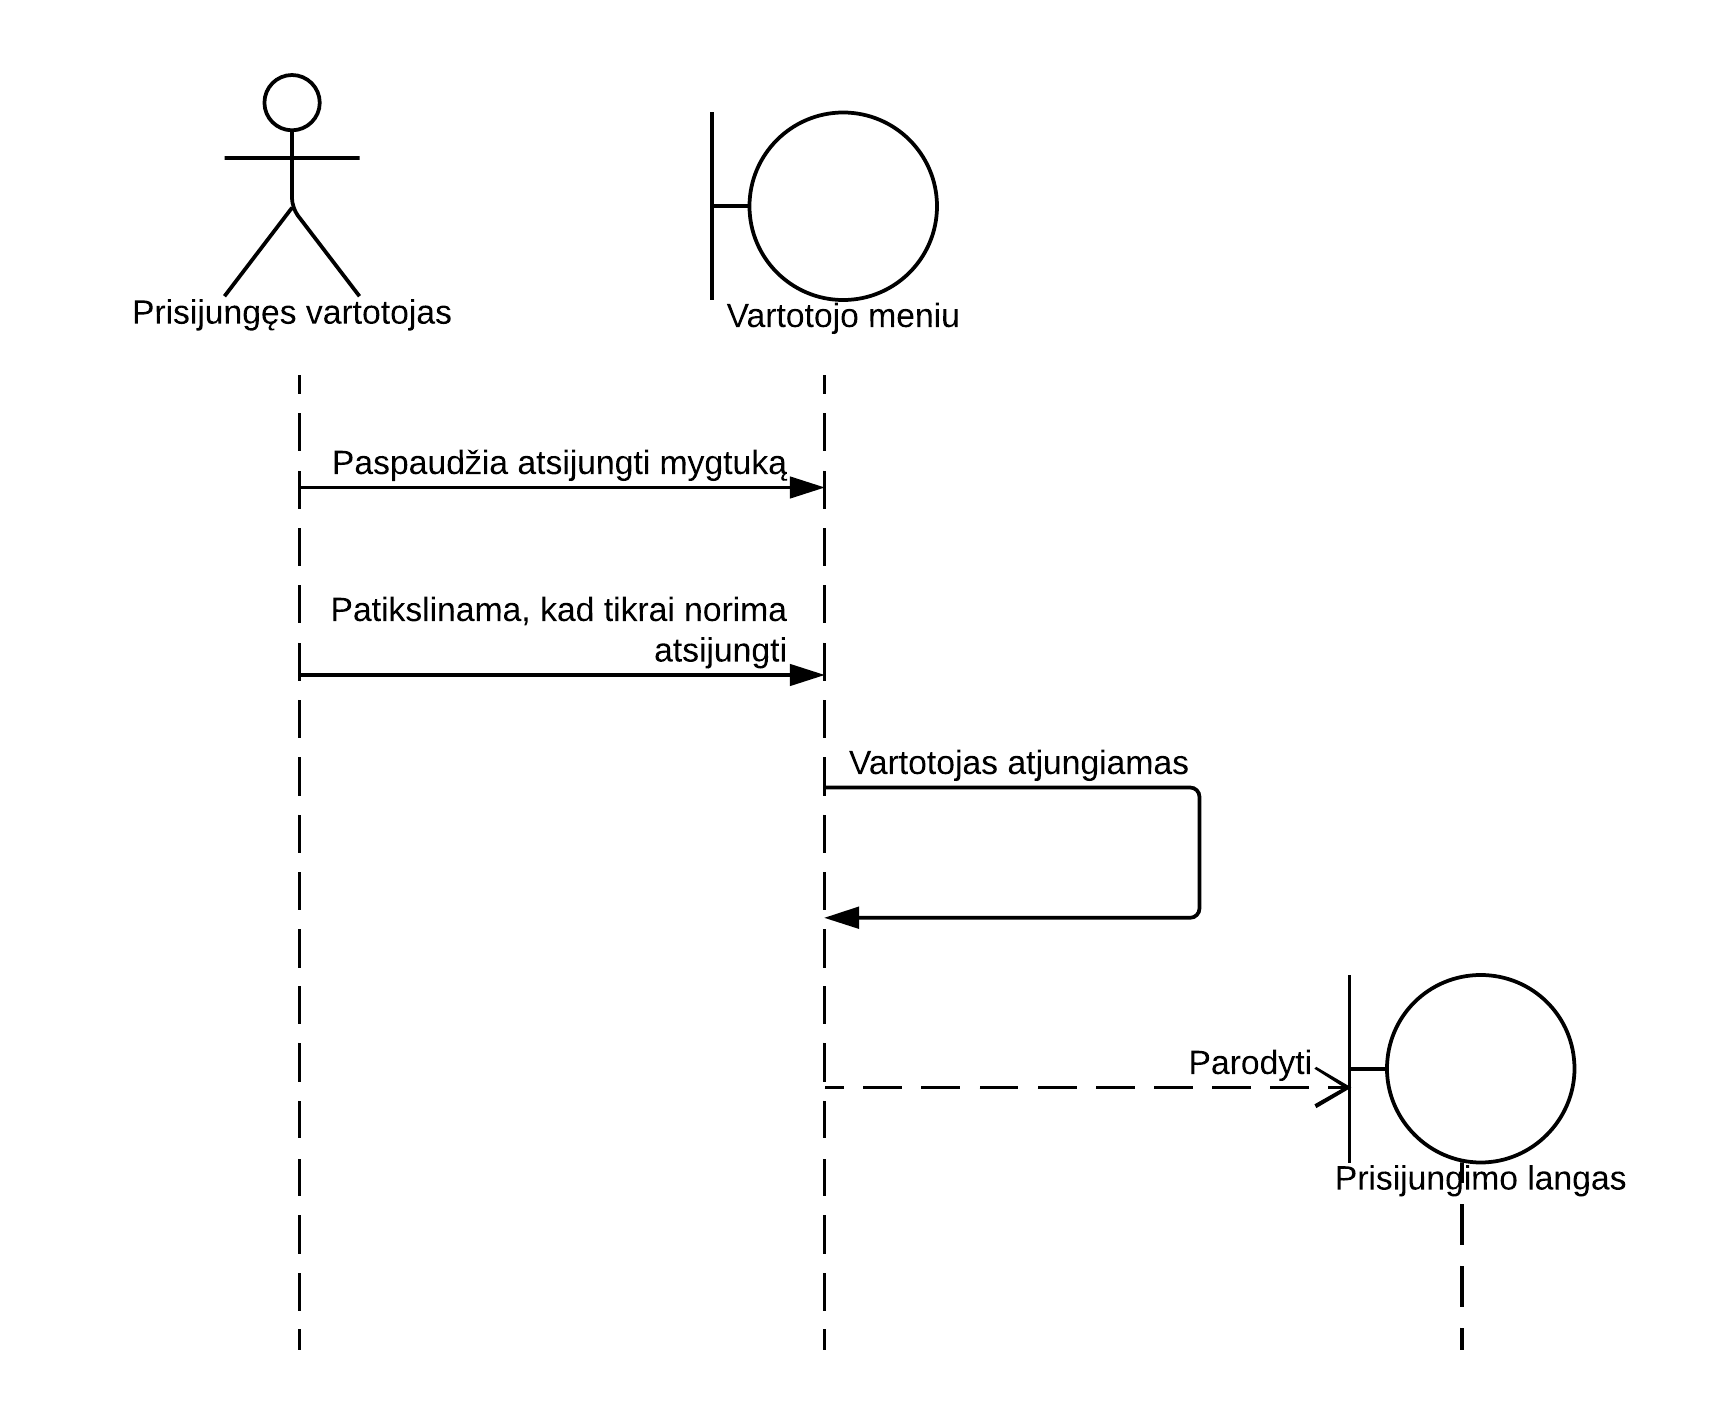
\includegraphics[width=1\textwidth]{Sekos_diagramos/atsijungti_seq_diag}
    \caption{atsijungimo diagrama}
\end{figure}

\pagebreak

\subsection{Darbuotojo scenarijai}
Šiame poskyryje yra pateikiam darbuotojo atliekami užduočių pagrindiniai ir alternatyvūs scenarijai (žr. \ref{fig:ucDarb}).

\begin{figure}[H]
\label{fig:ucDarb}
    \centering
    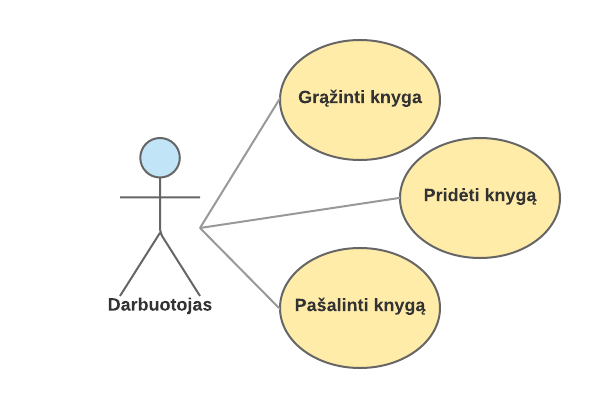
\includegraphics[width=1\textwidth]{vidines/ucDarb}
	\caption{Darbuotojo užduočių diagrama}
\end{figure}

\pagebreak

\subsubsection{Grąžinti knygą U7}

\begin{comment}

\begin{figure}[H]
\caption{Darbuotojo knygos grąžinimo sekų diagrama}
\label{fig:procesu2}
    \centering
    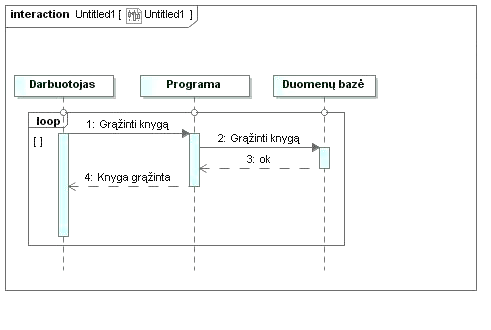
\includegraphics[width=1\textwidth]{diagramos/procesu2}

\end{figure}

	\textbf{Pagrindinis scenarijus:} Skaitytojas atėjęs ar kitaip nugabenęs knygą į biblioteką, ją atiduoda. Jei knyga nėra grąžinta pavėluotai - bibliotekininkas paima knygą, programoje nusigauna iki knygos grąžinimo lango ir įveda jos ID numerį. Jei knygą grąžinama pavėluotai, pranešama apie tai bibliotekininkui. Į duomenų bazę kreipiamasi su užklausa atlaisvinti knygą ir knyga tampa "laisva". Bibliotekininkas gauną pranešimą apie sėkmingai atlaisvintą knygą. 

	\textbf{Alternatyvūs scenarijai:} 
\begin{enumerate}
\item Darbuotojas įvedė neegzistuojanti ID numerį. Programa praneša, kad tokios knygos nėra. Darbuotojui leidžiama per naujo suvesti ID numerį.
\item Darbuotojas įvedė jau laisvos knygos numerį. Programa praneša, kad knyga jau yra "laisva". Darbuotojui leidžiama per naujo suvesti ID numerį.
\end{enumerate}

	\textbf{Nuoroda į reikalavimus:} FR.35 - FR.38

\end{comment}



	\textbf{Pagrindinis scenarijus :}
    
Skaitytojas atėjęs ar kitaip nugabenęs knygą į biblioteką, ją atiduoda. Jei knyga nėra grąžinta pavėluotai - bibliotekininkas paima knygą, programoje nusigauna iki knygos grąžinimo lango ir įveda jos ID numerį. Jei knygą grąžinama pavėluotai, pranešama apie tai bibliotekininkui. Į duomenų bazę kreipiamasi su užklausa atlaisvinti knygą ir knyga tampa "laisva". Bibliotekininkas gauną pranešimą apie sėkmingai gražintą knygą. 

	\textbf{Alternatyvūs scenarijai :}

	\begin{enumerate}
	\item Darbuotojas įvedė neegzistuojanti ID numerį. Programa praneša, kad tokios knygos nėra. Darbuotojas grąžinamas į knygos grąžinimo langą.
    
 	\item Darbuotojas įvedė jau laisvos knygos numerį. Programa praneša, kad knyga jau yra ”laisva”. Darbuotojas grąžinamas į knygos grąžinimo langą.
    
	\item Užklausa į duomenų bazė nesėkminga. Parodomas duomenų bazės klaidos langas. Darbuotojas grąžinamas į knygos grąžinimo langą.
    
    \item Knyga bandoma grąžinti pavėluotai. Darbuotojui pateikiamas knygos grąžinimo vėlavimo langas su nurodytu vėlavimo laiku. Darbuotojas patvirtina sumokėtą baudą.
  	 \end{enumerate}  
 	\textbf {Nuoroda į reikalavimus :} FR.35 - FR.38

\begin{figure}[H] 
    \label{fig:bookretdiag}
    \centering
    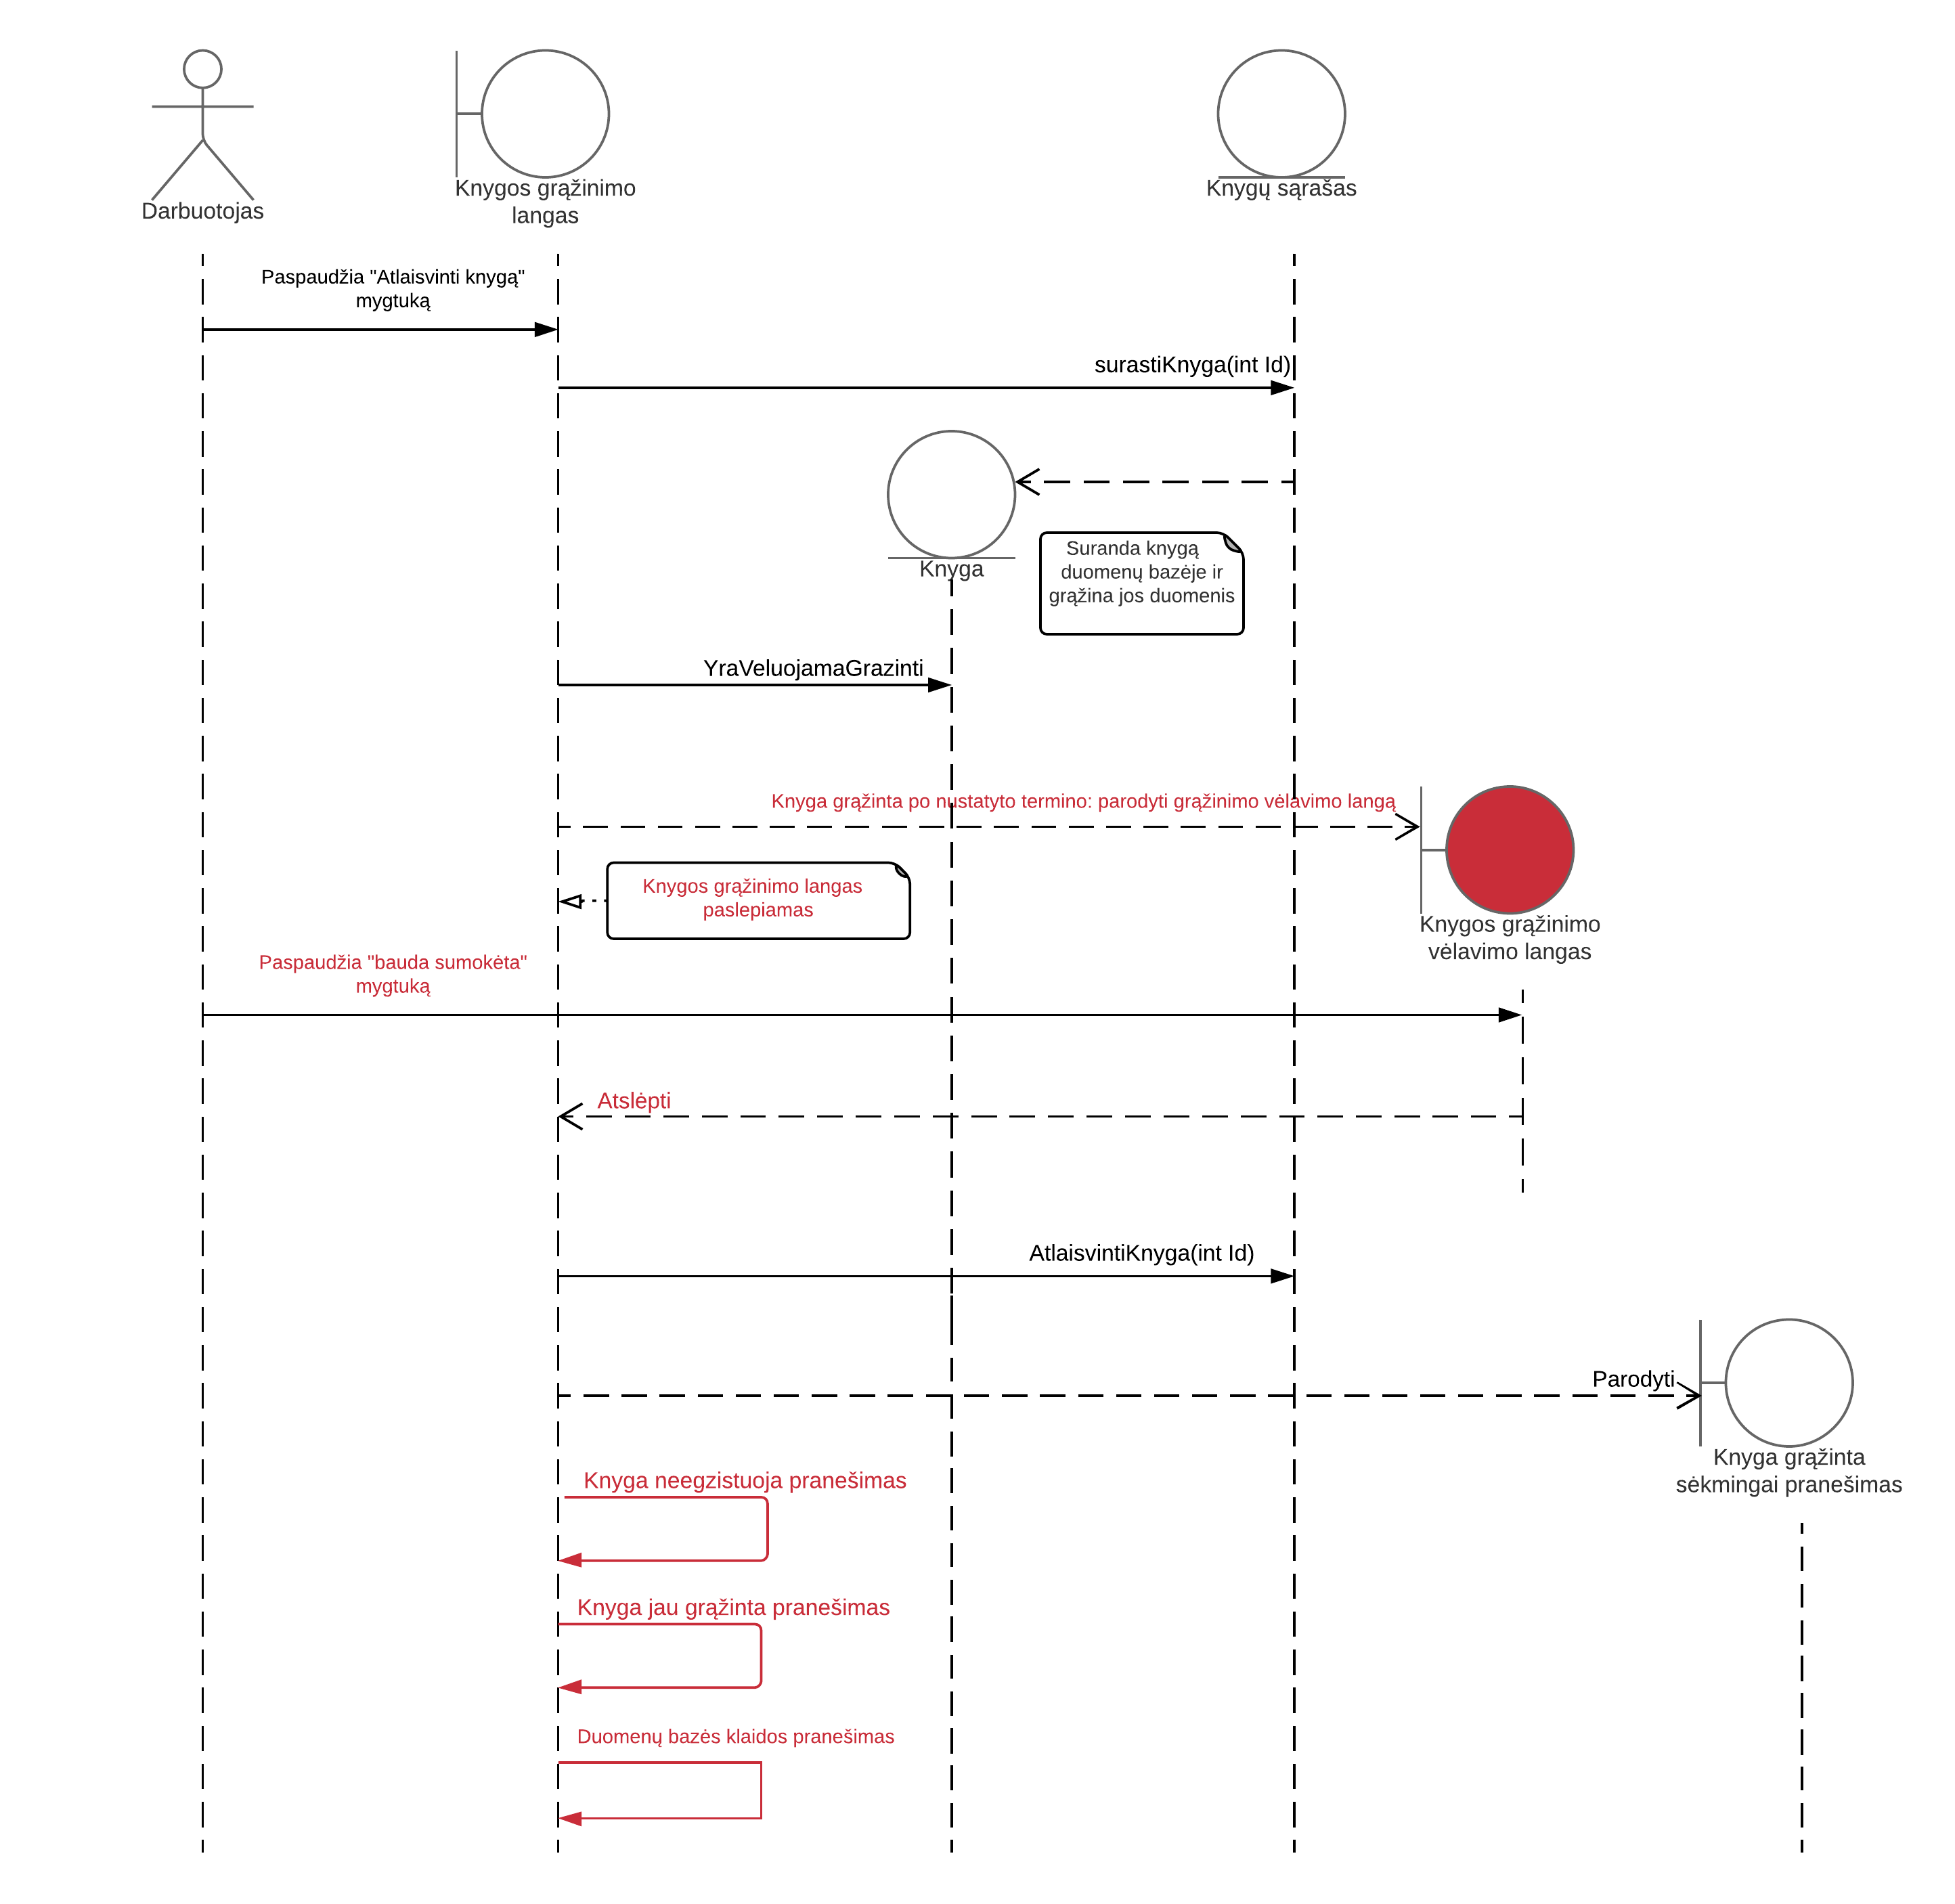
\includegraphics[width=1.1\textwidth]{Sekos_diagramos/grazinti_knyga_seq_diag}
    \caption{knygos grąžinimo bibliotekos diagrama}
\end{figure}

\subsubsection{Pridėti knygą U8}

\begin{comment}

\begin{figure}[H]
\caption{Darbuotojo knygos pridėjimo sekų diagrama}
\label{fig:procesu4}
    \centering
    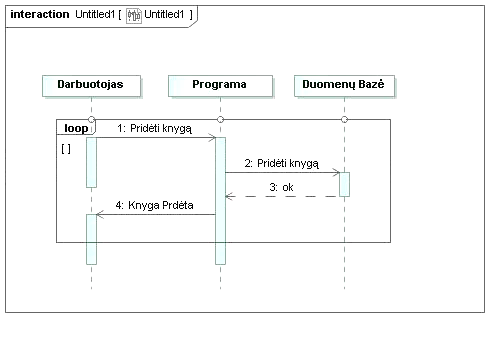
\includegraphics[width=1\textwidth]{diagramos/procesu4}

\end{figure}

\end{comment}

\begin{figure}[H]
\label{fig:pridetknygalang}
    \centering
    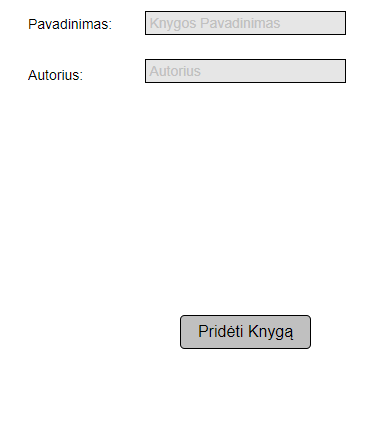
\includegraphics[width=1\textwidth]{vidines/ucpridetiknyga}
	\caption{Knygos pridėjimo langas}
\end{figure}

\begin{comment}
\textbf{Tikslas:} Užregistruoti knygą, kurios dar nėra duomenų bazėje ir padaryti ją prieinamą skaitytojams (ir rezervacijai).

	\textbf{Pagrindinis scenarijus:} Nusigaunama iki "pridėti knygą" lango (žr. \ref{fig:pridetknygalang}) ; įvedamas bent knygos pavadinimas ir autorius. Užklausa sukurti įrašą siunčiama į duomenų bazę. Duomenų bazė atgal grąžina pranešimą apie sėkmingą operaciją ir parodo naujo įrašo ID kodą.

	\textbf{Alternatyvūs scenarijai:} 
\begin{enumerate}
\item Duomenų bazė yra nepasiekiama arba grąžiną klaidos pranešimą. Bibliotekos darbuotojui pranešama jog įvyko klaida, jis grąžinamas į "pridėti knygą" langą.
\item Duomenys neatitinka minimalių duomenų reikalavimo arba yra netinkamo formato. Darbuotojui pranešama kur padaryta klaida, siūloma pakeisti įvestus duomenis, kol jie atitinka reikalavimus.
\end{enumerate}

\textbf{Nuoroda į reikalavimus:} FR.44 - FR.47
\end{comment}




	\textbf{Pagrindinis scenarijus :} 
    
    Nusigaunama iki ”pridėti knygą” lango; įvedamas bent knygos pavadinimas ir autorius.  Užklausa sukurti įrašą siunčiama į duomenų bazę. Duomenų bazė atgal grąžina pranešimą apie sėkmingą operaciją ir parodo naujo įrašo ID kodą.	
    
    \textbf{Alternatyvūs scenarijai :} 
	\begin{enumerate}
	\item Duomenų bazė yra nepasiekiama arba grąžiną klaidos pranešimą. Bibliotekos darbuotojui pranešama jog įvyko klaida, jis grąžinamas į ”pridėti knygą” langą. 
    
    \item Duomenys neatitinka minimalių duomenų reikalavimo arba yra netinkamo formato. Darbuotojui pranešama kur padaryta klaida, siūloma pakeisti įvestus duomenis, kol jie atitinka reikalavimus.
    \end{enumerate}
    
      \textbf {Nuoroda į reikalavimus :} FR.44 - FR.47

\begin{figure}[H]
    \label{fig:bookadddiag}
    \centering
    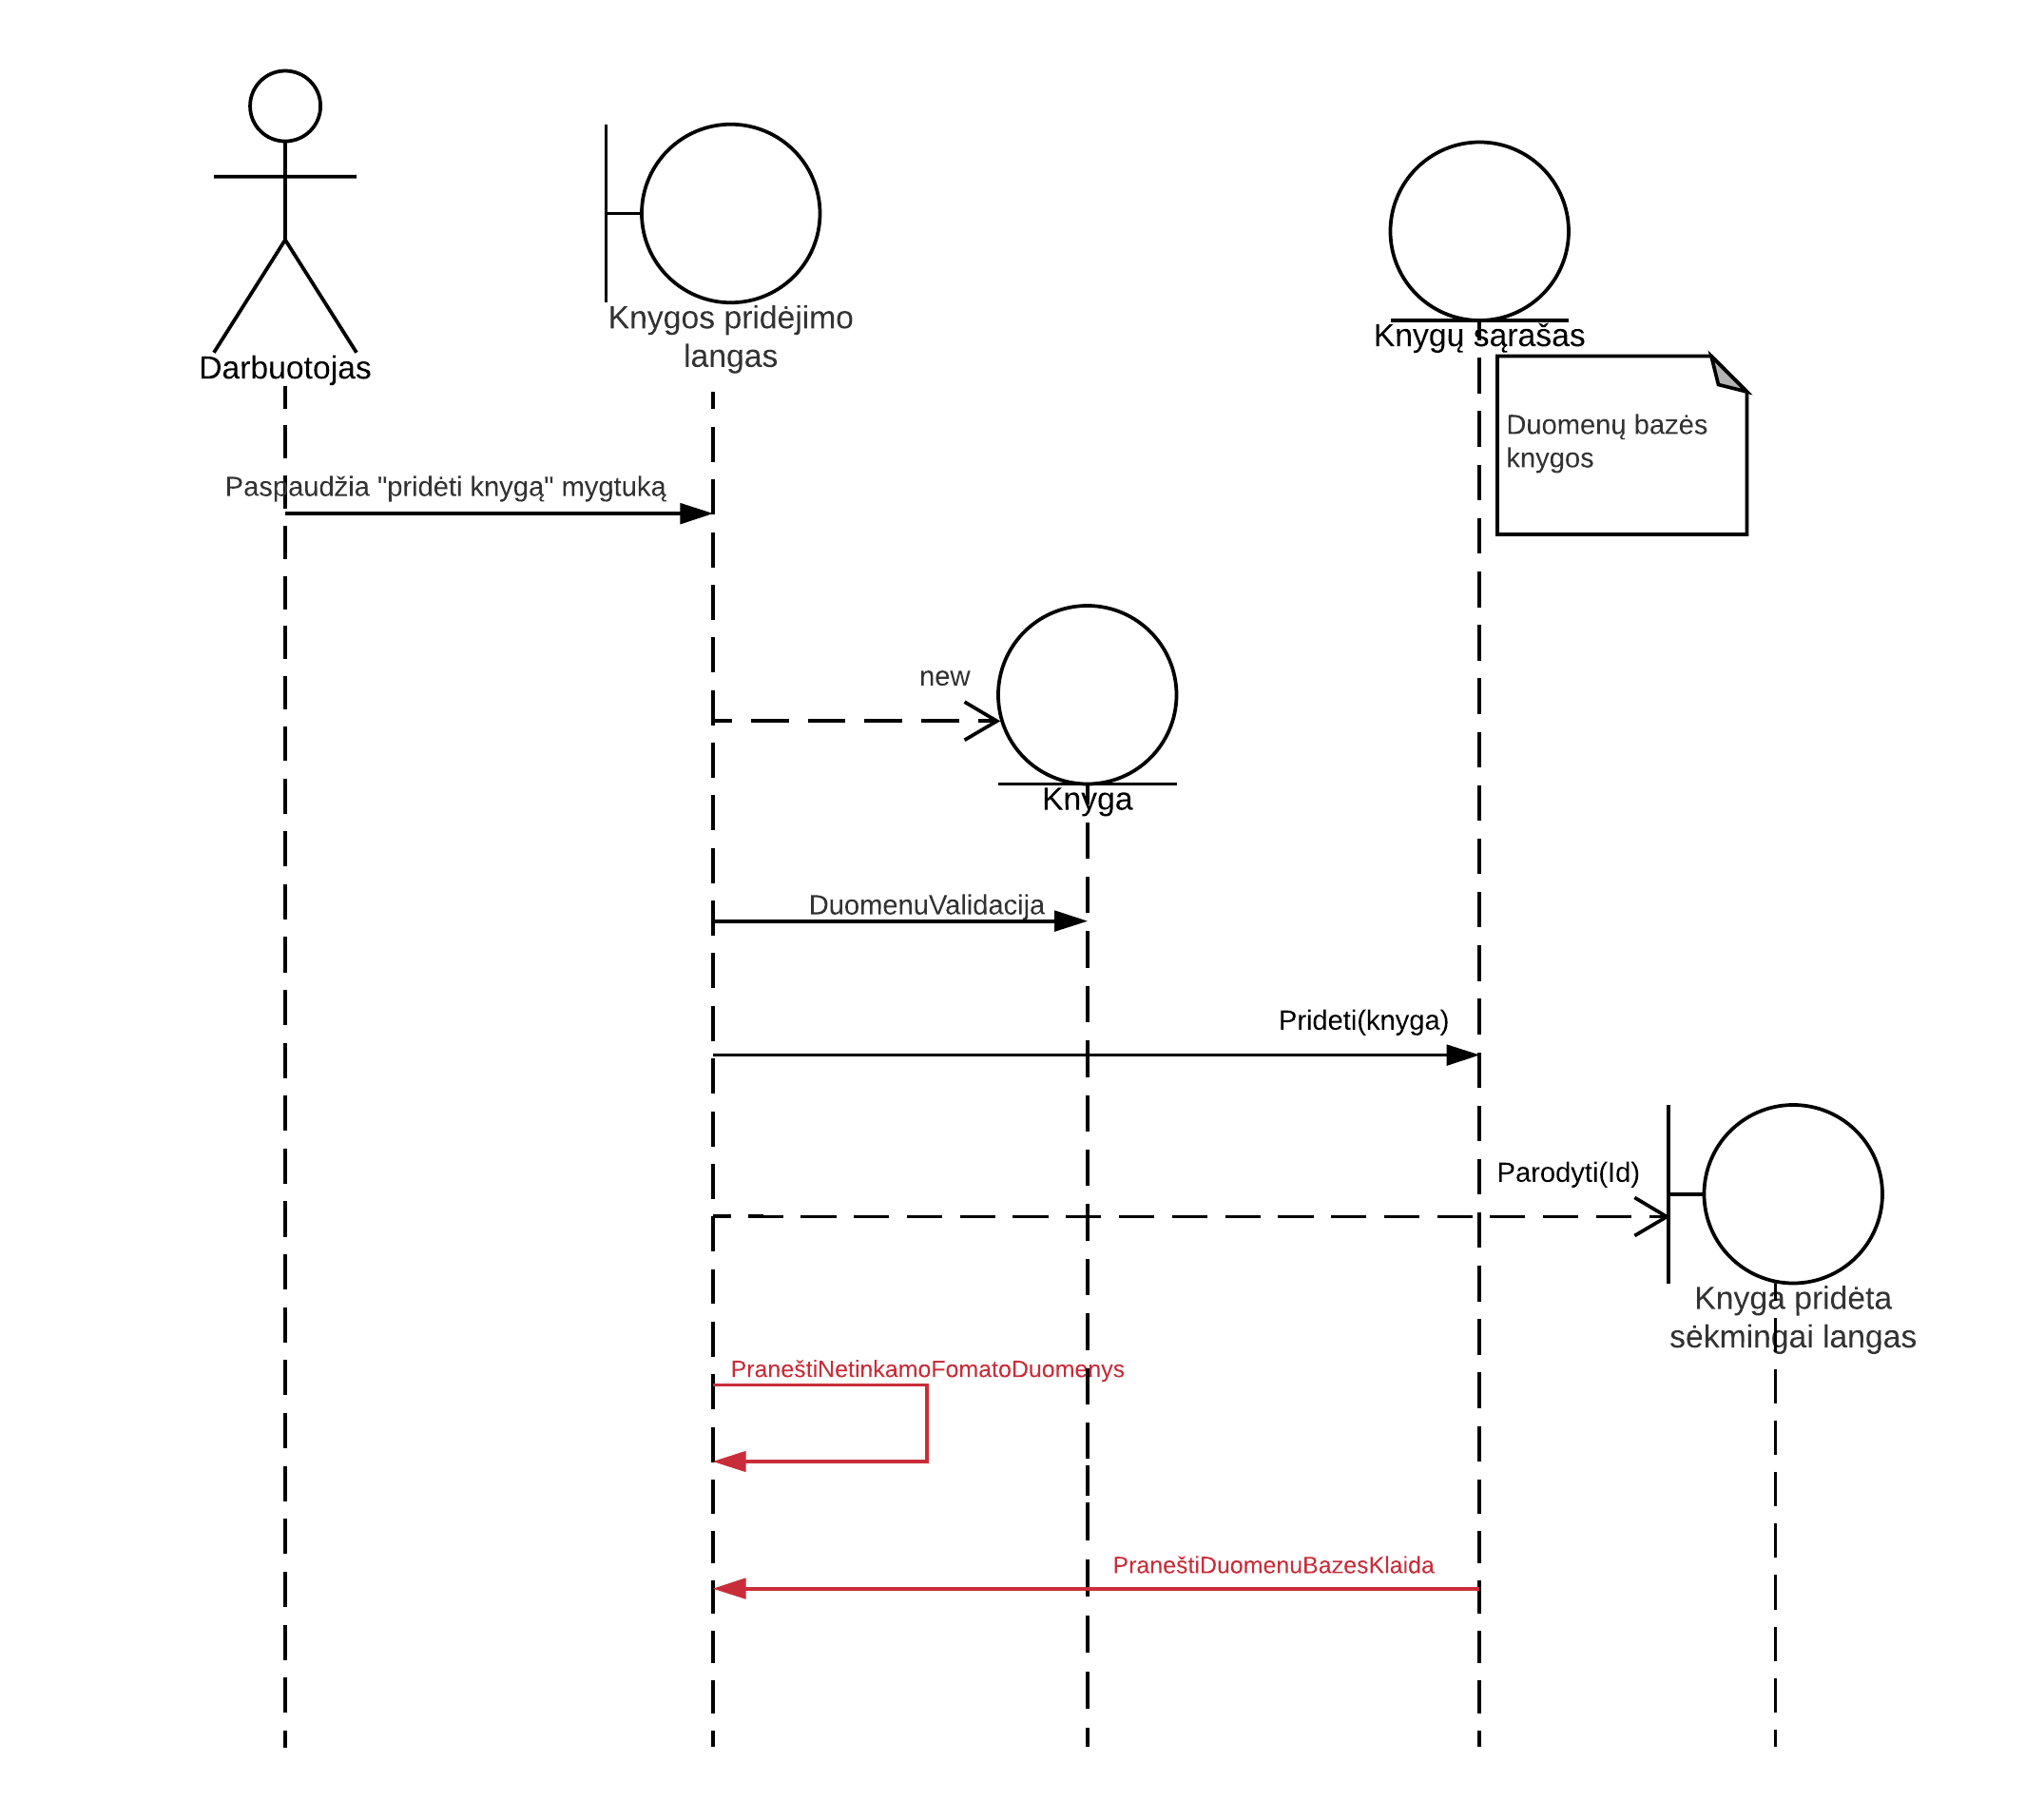
\includegraphics[width=1.05\textwidth]{Sekos_diagramos/prideti_knyga_seq_diag}
    \caption{knygos pridėjimo į biblioteką diagrama}
\end{figure}
 
\subsubsection{Knygos šalinimas iš sistemos U9}

\begin{comment}

\begin{figure}[H]
\caption{Knygos šalinimo iš sistemos sekų diagrama}
\label{fig:Delete}
    \centering
    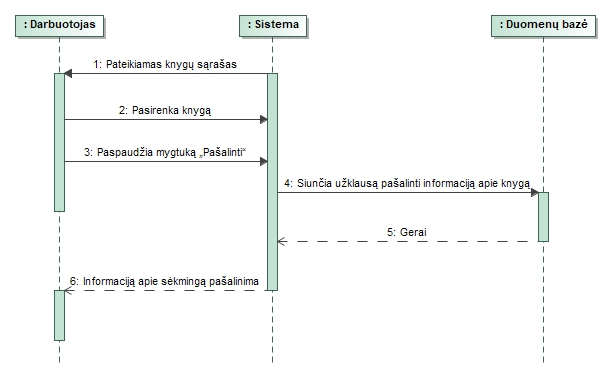
\includegraphics[width=1\textwidth]{diagramos/Delete}

\end{figure}

	\textbf{Tikslas:} Pašalinti knygą iš sistemos.

	\textbf{Pagrindinis scenarijus :} Darbuotojui pateikiamas knygų sąrašas, iš kurio jis pasirenka knygą, kurią nori pašalinti iš sistemos. Tada jis paspaudžia mygtuką „Pašalinti“, o sistema siunčia užklausą į duomenų bazę, kad būtų pašalinta informaciją apie knygą. Sistema praneša darbuotojui apie sėkmingą knygos pašalinimą iš sistemos.

	\textbf{Alternatyvūs scenarijai:} Žr. FR 49.

	\textbf{Nuoroda į reikalavimus:} FR.48.-FR.50.
\end{comment}

    
    \textbf {Pagrindinis scenarijus :}
    
    Darbuotojas knygos duomenų lange paspaudžia mygtuką „Pašalinti“. Sistema paklausia ar tikrai norite pašalinti knygą ir parodo knygos ID numerį. Darbuotojui patvirtinus, sistema siunčia užklausą į duomenų bazę, kad būtų pašalintas knygos egzempliorius. Sistema praneša darbuotojui apie sėkmingą knygos pašalinimą iš sistemos.

    \textbf {Alternatyvūs scenarijai :}
    	\begin{enumerate}
	\item Knyga yra paimta: parodomas pranešimas, kad knyga šiuo metu paskolinta. Darbuotojas grąžinamas į knygos duomenų langą.

	\item Knyga yra rezervuota: knygos ištrinimo lange parodomas pranešimas, kad kažkurio vartotojo rezervacija bus atšaukta. Darbuotojui patvirtinus knygus ištrinimą, knyga pašalinama iš sistemos.

 	\item Sistemai paklausus "ar tikrai norite pašalinti knygą?" darbuotojas paspaudžia "ne". Yra grąžinamas atgal į knygos duomenų langą.
\end{enumerate}

	\textbf {Nuoroda į reikalavimus :} FR.48.-FR.50.
  \begin{figure}[H]
    \label{fig:bookremovediag}
    \centering
    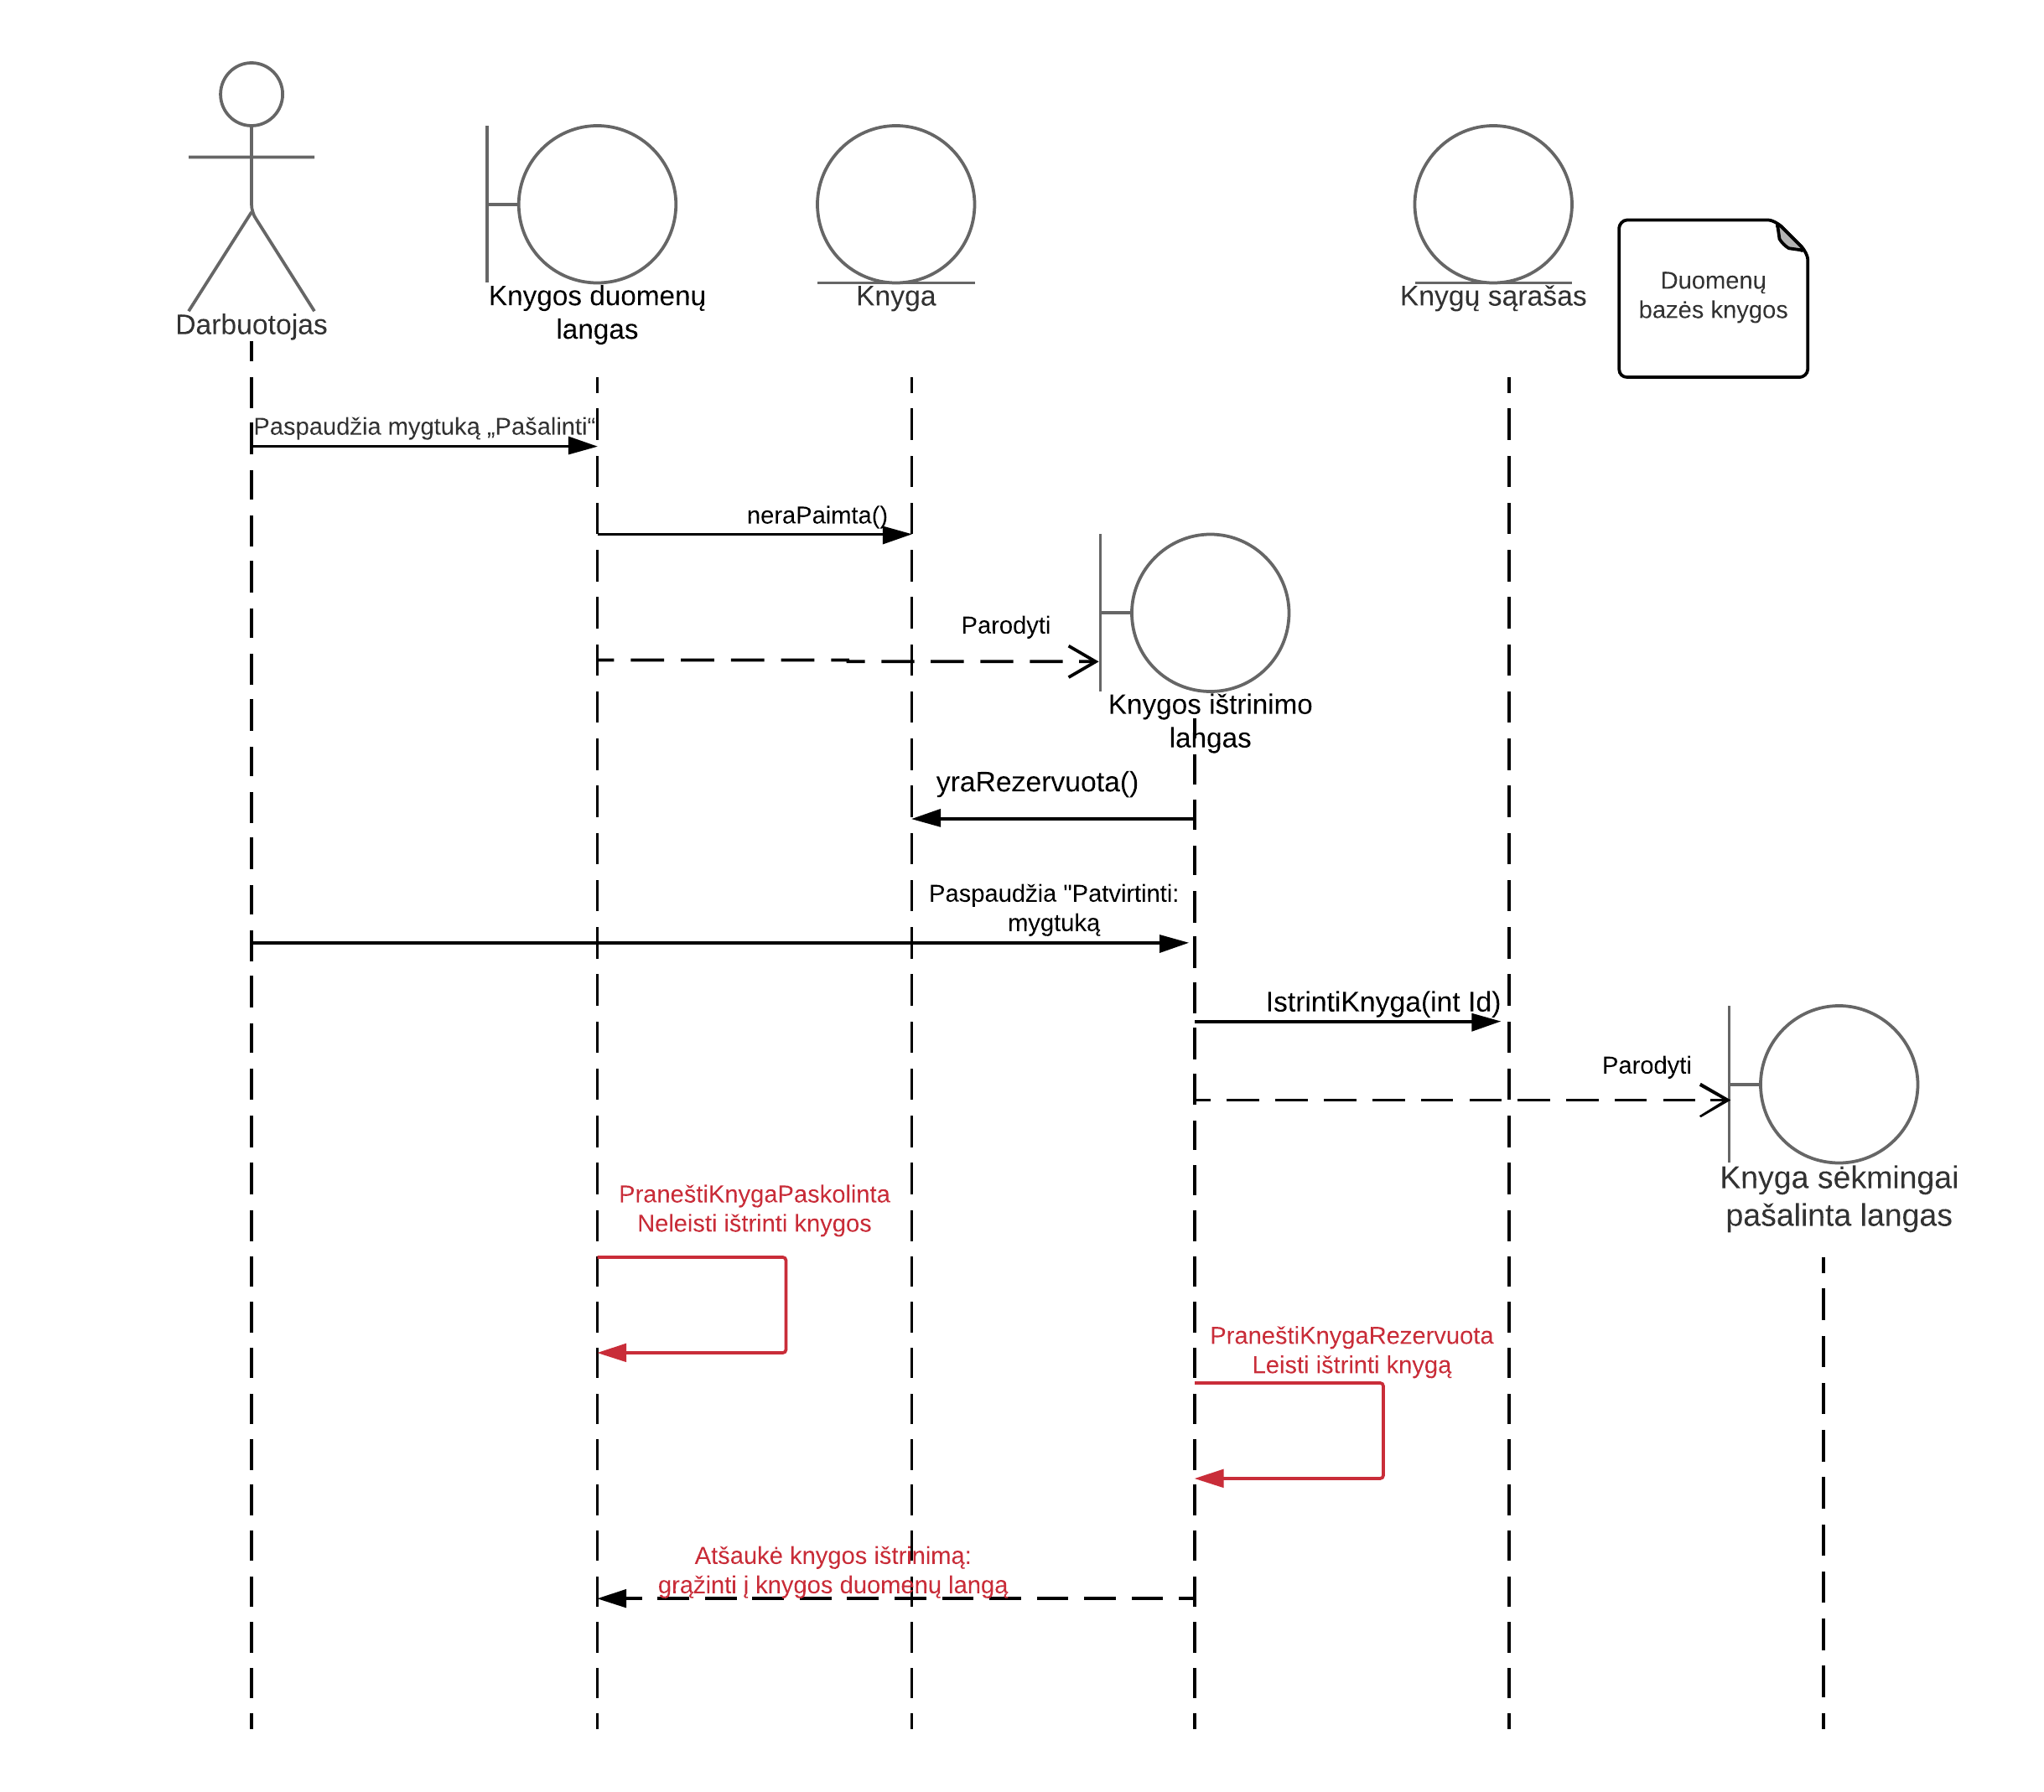
\includegraphics[width=1.05\textwidth]{Sekos_diagramos/istrinti_knyga_seq_diag}
    \caption{knygos ištrinimas iš bibliotekos diagrama}
\end{figure}  
    
\subsection{Reikalavimų - užduočių matrica. }
Šiame poskyryje pateikiama reikalavimų - užduočių atsekamumo matrica (žr. \ref{fig:uzdmatr}).    
    
\begin{figure}[H]
\label{fig:uzdmatr}
    \centering
    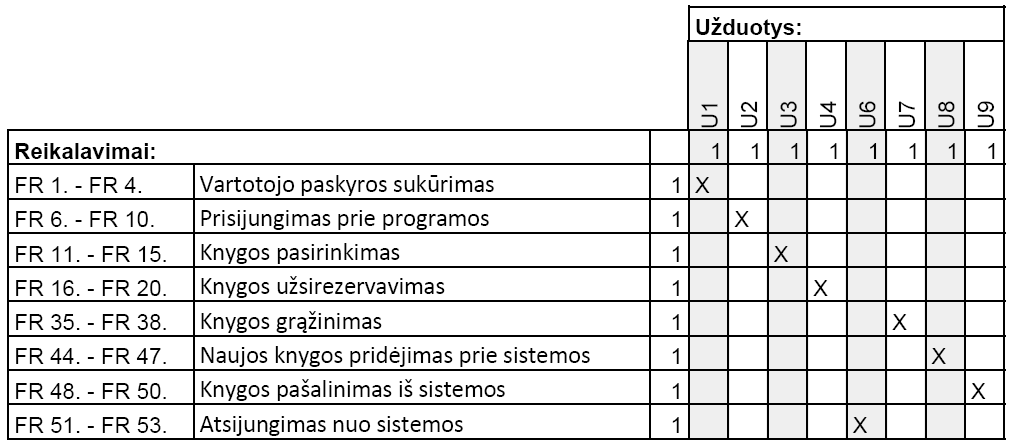
\includegraphics[width=1\textwidth]{matricos/uzdmat}
	\caption{Darbuotojo knygos pridėjimo sekų diagrama}
\end{figure}

%technine architektura
\section{Techinė architektūra}
Šiame skyriuje pateikta informacija apie sistemos techninės architektūros peržiūra.
\subsection{Vidiniai komponentai}

\begin{figure}[H]  
    \label{fig:innerComponents}
    \centering
    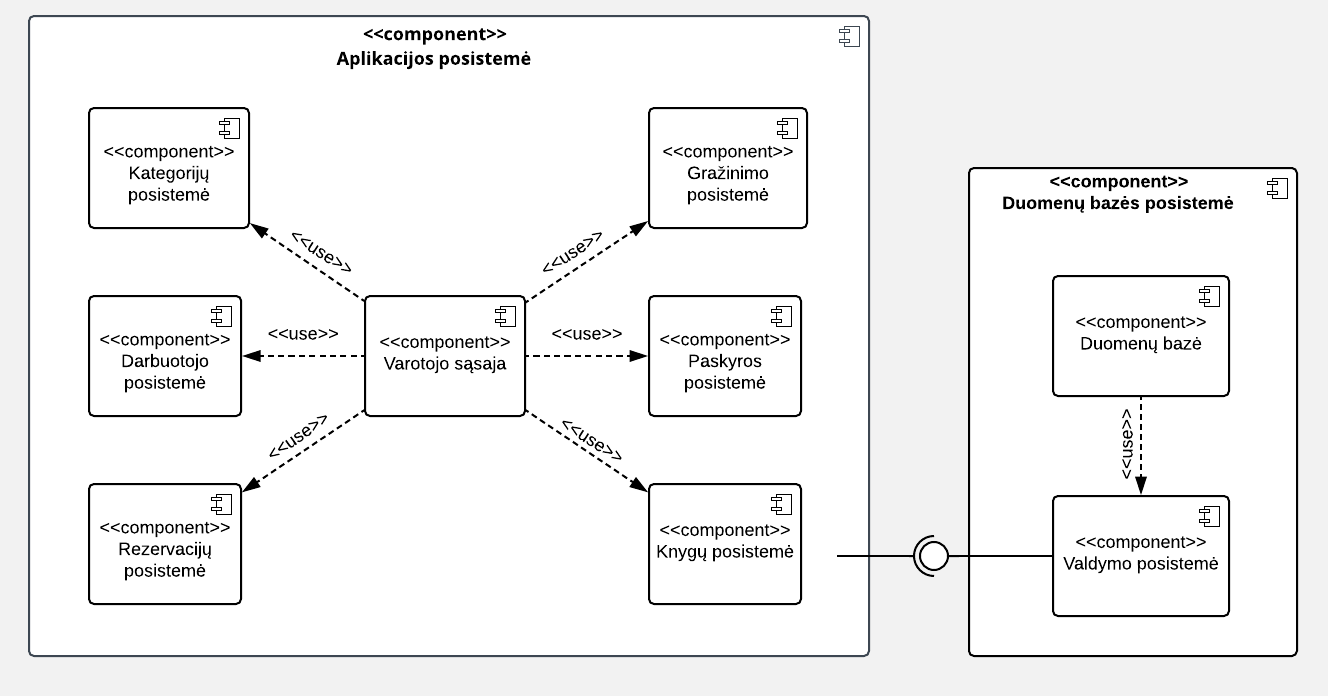
\includegraphics[width=1.1\textwidth]{Robastiskumo/innerComponents}
    \caption{Vidinių komponentų diagrama}
\end{figure}

Bibliotekos programelę sudaro dvi posistemės – aplikacijos ir duomenų bazės.
Duomenų bazės posistemėje yra duomenų bazė, kur saugomi sistemos duomenys, ir valdymo
posistemė, kuri atlieka duomenų bazių ir kitas užklausas bei jungiasi su aplikacijos posisteme.
Aplikacijos posistemėje yra vartotojo sąsaja, kuri pasitelkdama likusias posistemes (Kategorijų, darbuotojo, rezervacijų, gražinimo, paskyros ir knygų) ir jų metodus parūpina informaciją vartotojui
bei pateikia ją grafiniu būdu.

\subsection{Komponentų išdėstymas tinkle, jų saugumas}

\begin{figure}[H]
    \label{fig:networkComponents}
    \centering
    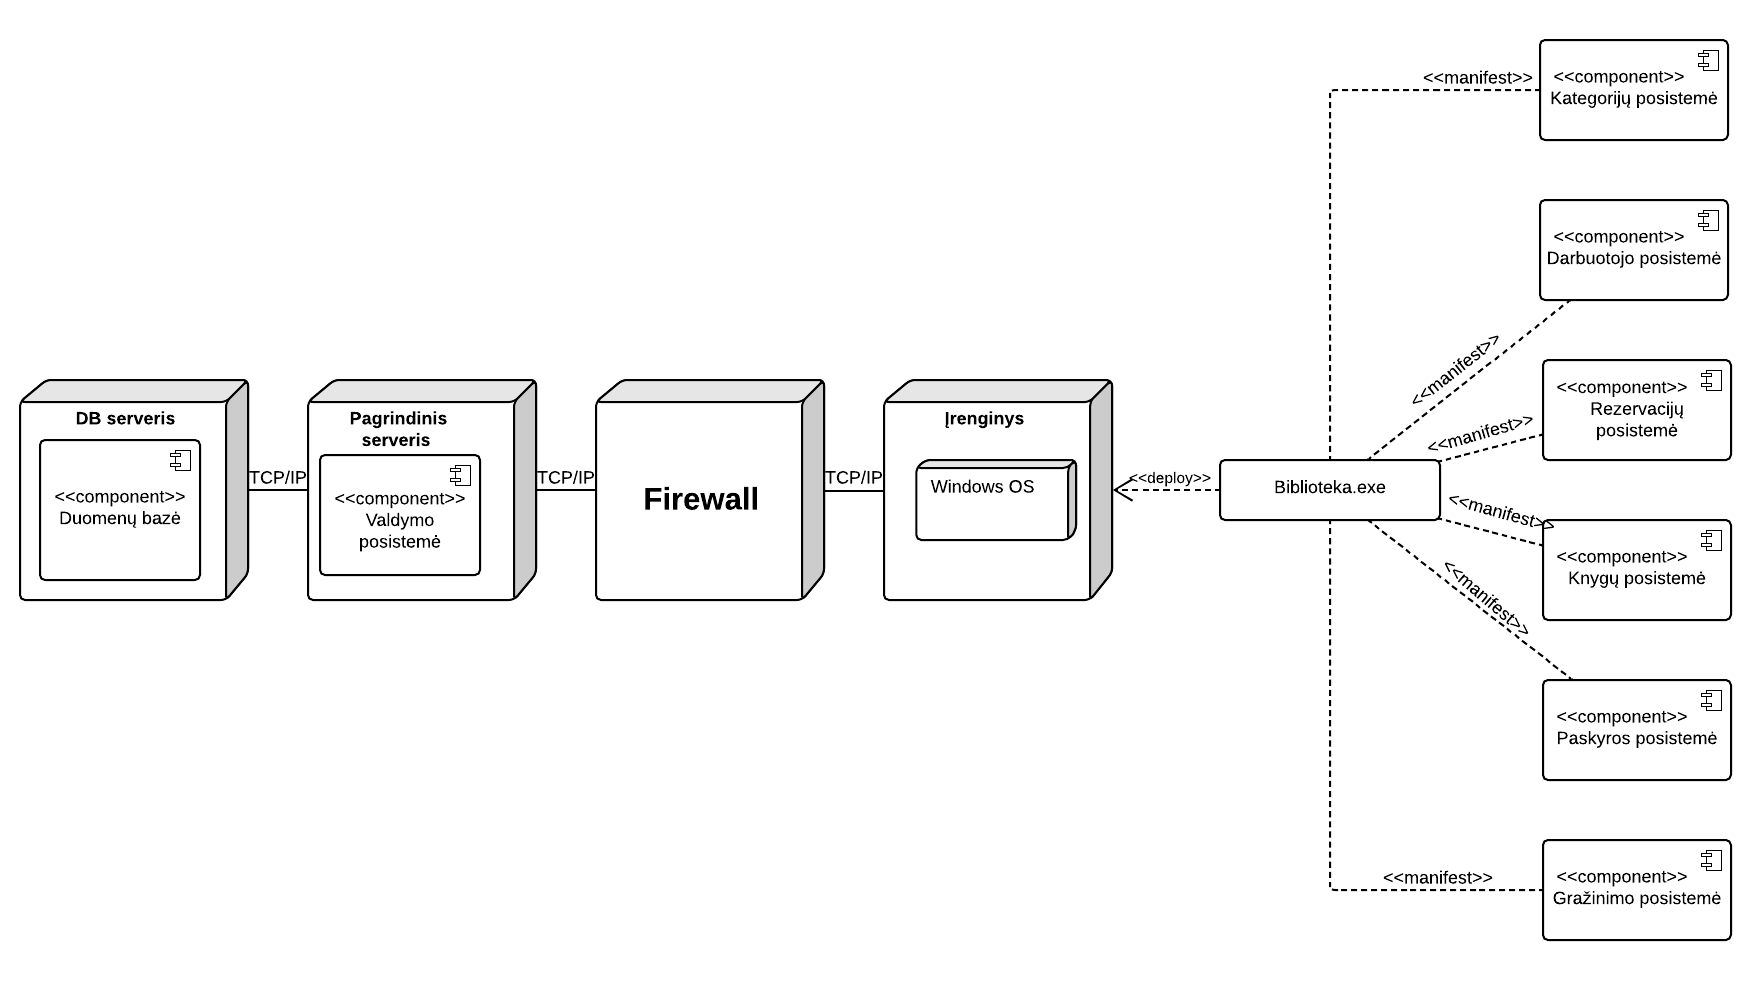
\includegraphics[width=1 \textwidth]{Robastiskumo/networkComponents}
    \caption{Komponentų išsidėstymas tinkle}
\end{figure}

Maisto pristatymo sistemoje yra du serveriai, viename jų yra duomenų bazė su
duomenimis, kitame – valdymo posistemė, kuri valdo duomenų srautą sistemoje. Taip pat yra
įrenginys su įrašyta Windows operacine sistema bei Bibliotekos aplikacija, kurioje
veikia anksčiau minėtos posistemės. Aplikacijos naudotojas gali būti darbuotojas arba skaitytojas.
Įrenginiai su pagrindiniu serveriu bei duomenų bazės ir pagrindinis serveriai tarpusavyje siejasi
TCP/IP ryšiu, kurio srautą prižiūri ugniasienė saugodama nuo nuotolinių atakų – bandymo
išgauti duomenis, kenkėjiškų programų palikimo ar kitos potencialios žalos sistemai.

\subsection{Diegimas ir palaikymas}
Aplikacijos kūrėjai turės dedikuotą žmogų, kuris atliks diegimą bibliotekai, kuri nuspręs naudotis bibliotekos aplikaciją. Pirmojo diegimo metu yra įrašoma naujausia aplikacijos versija. Atnaujinimas ir aplikacijos palaikymas vyks nuotoliniu būdu. 


\section{Testavimo planas ir scenarijai}

Šiame skyriuje pateikiami užduočių pagrindu sukurti testavimo planai (žr pav. 19 ir 20). Raudona spalva pažymėti alternatyvieji scenarijai. 


\begin{figure}[H]
    \label{fig:testavimoscenarijai}
    \centering
    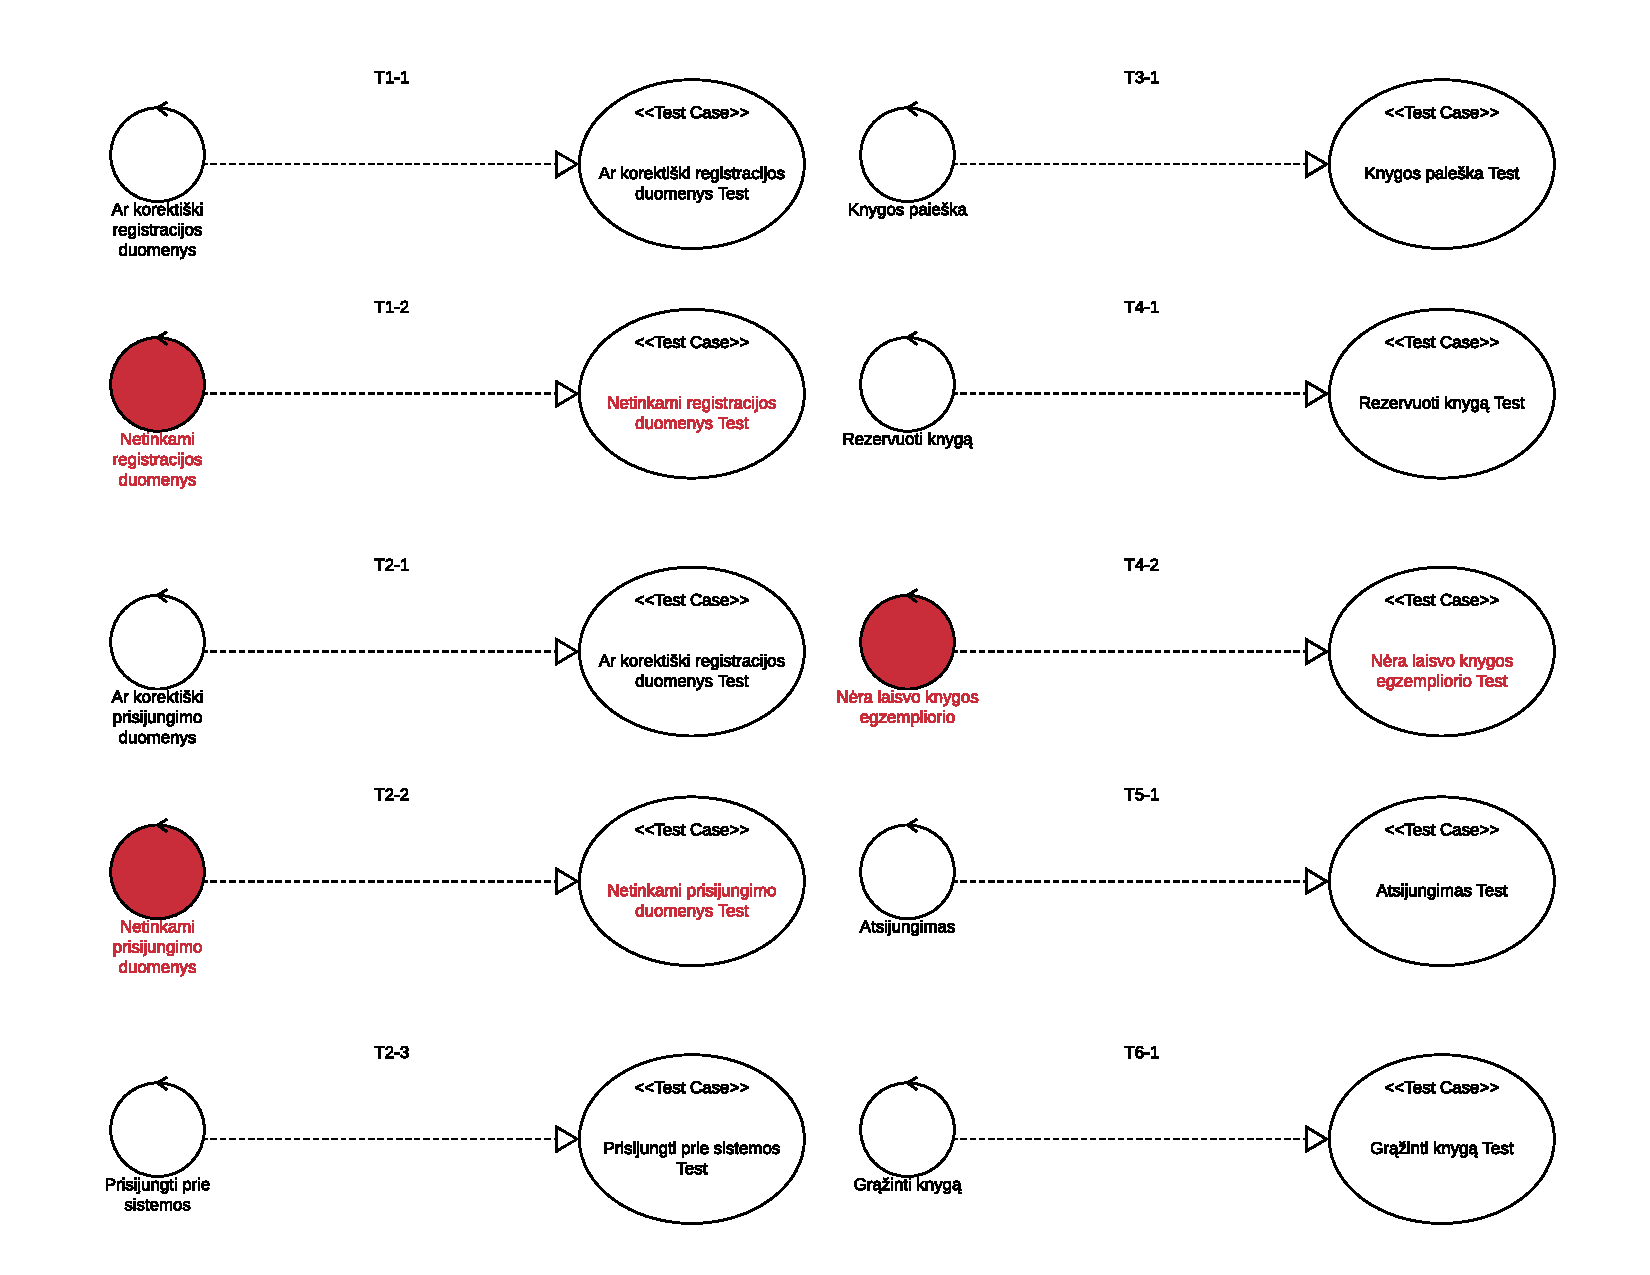
\includegraphics[page = 1, width=1.1 \textwidth]{Testavimo_Scenarijai/TestavimoScenarijai}
    \caption{Testavimo scenarijai}
\end{figure}

\begin{figure}[H]
    \label{fig:testavimoscenarijai2}
    \centering
    \includegraphics[page = 2, width=1.1 \textwidth]{Testavimo_Scenarijai/TestavimoScenarijai}
    \caption{Testavimo scenarijai, tęsinys}
\end{figure}

\subsection*{1 užduotis. Registracija}
\textbf{Testai:}

\begin{enumerate}
\item Pagrindinis scenarijus
\item Registracija, kai įvesti netinkami duomenys
\item Registracija, kai nėra įvestų duomenų
\item Registracija, kai toks vartuotojas jau egzistuoja
\end{enumerate}
\hfill \break
\textbf{Testas 1-1}\\
\hfill \break
\textbf{Tikslas:} Ar veikia pagrindinis scenarijus? (Žr. pav. 19, T 1-1 diagramą)
\hfill \break
\hfill \break
\textbf{Prieš sąlygos:} aplikacija įrašyta į kompiuterį, atidarytas registracijos langas.
\hfill \break
\hfill \break
\textbf{Žingsniai:}
\hfill \break
\begin{enumerate}
\item Korektiškai užpildyti privalomus registracijos laukus: (žr. FR 1)
\begin{itemize}
\item Pasirinkti darbuotojo ar skaitytojo paskyrą
\item Prisijungimo vardas
\item Slaptažodis
\end{itemize}
\item Paspaust mygtuką "Registruotis"
\item Patikrinti, ar paskyra sukurta ir buvote nukreiptas į pagrindinį bibliotekos langą.
\end{enumerate}
\textbf{Testas 1-2}\\
\hfill \break
\textbf{Tikslas:} Patikrinti, kaip elgiasi programa, kai įvesti netinkami registracijos duomenys (Žr. pav. 19, T 1-2 diagramą)
\hfill \break
\hfill \break
\textbf{Prieš sąlygos:} aplikacija įrašyta į kompiuterį, atidarytas registracijos langas.
\hfill \break
\hfill \break
\textbf{Žingsniai:}
\hfill \break
\begin{enumerate}
\item Nekorektiškai užpildyti privalomus registracijos laukus
\item Paspaust mygtuką "Registruotis"
\item Patikrinti, ar programa atpažino nekorektiškai įvestus duomenys ir apie tai informavo naudotoją.
\end{enumerate}
\textbf{Testas 1-3}\\
\hfill \break
\textbf{Tikslas:} Patikrinti, kaip elgiasi programa, kai nėra įvestų jokių duomenų (Žr. pav. 19, T 1-2 diagramą)
\hfill \break
\hfill \break
\textbf{Prieš sąlygos:} aplikacija įrašyta į kompiuterį, atidarytas registracijos langas.
\hfill \break
\hfill \break
\textbf{Žingsniai:}
\hfill \break
\begin{enumerate}
\item Paspaust mygtuką "Registruotis"
\item Patikrinti, ar programa atpažino tusčius privalomus laukus ir apie tai informavo naudotoją.
\end{enumerate}
\textbf{Testas 1-4}\\
\hfill \break
\textbf{Tikslas:} Patikrinti, kaip elgiasi programa, kai vartotojo vardas jau egzistuoja (Žr. pav. 19, T 1-2 diagramą)
\hfill \break
\hfill \break
\textbf{Prieš sąlygos:} aplikacija įrašyta į kompiuterį, atidarytas registracijos langas.
\hfill \break
\hfill \break
\textbf{Žingsniai:}
\hfill \break
\begin{enumerate}
\item Pakartoti visus žingsnius iš 1-1 Testo (sukūrt naudotoją).
\item Atidaryti naują registracijos langą
\item Pabandyti sukūrt vartotoją su tuo pačiu vardu kaip prieš tai buvo kurtas.
\item Patikrinti, ar programa rado jau egzistuojantį vartotoją ir apie tai informavo naudotoją.
\end{enumerate}

\subsection*{2 užduotis. Prisijungimas}
\textbf{Testai :}

\begin{enumerate}
\item Pagrindinis scenarijus
\item Kai įvesti neteisingi prisijungimo duomenys
\item Kai nėra įvestų duomenų
\item Kai yra pasirinkta skaitytojo paskyra bet įvesti darbuotojo prisijungimo duomenys (ir atvirksčiai)
\end{enumerate}
\hfill \break
\textbf{Testas 2-1}\\
\hfill \break
\textbf{Tikslas:} Ar veikia pagrindinis scenarijus? (Žr. pav. 19, T 2-1 diagramą)
\hfill \break
\hfill \break
\textbf{Prieš sąlygos:} aplikacija įrašyta į kompiuterį, atidarytas prisijungimo langas.
\hfill \break
\hfill \break
\textbf{Žingsniai:}
\hfill \break
\begin{enumerate}
\item Korektiškai užpildyti privalomus prisijungimo laukus: (žr. FR 6)
\begin{itemize}
\item Pasirinkt darbuotojo ar skaitytojo paskyrą
\item Teisingas prisijungimo varads
\item Teisingas slaptažodis
\end{itemize}
\item Paspaust mygtuką "Prisijungti"
\item Patikrinti, ar prisijungimas buvo sėkmingas ir buvote nukreiptas į pagrindinį sistemos langą.
\end{enumerate}
\hfill \break
\textbf{Testas 2-2}\\
\hfill \break
\textbf{Tikslas:} Patikrinti, ar sistemą korektiškai apdoroją kai yra įvesti nekorektiški prisijungimo duomenys? (Žr. pav. 19, T 2-2 diagramą)
\hfill \break
\hfill \break
\textbf{Prieš sąlygos:} aplikacija įrašyta į kompiuterį, atidarytas prisijungimo langas.
\hfill \break
\hfill \break
\textbf{Žingsniai:}
\hfill \break
\begin{enumerate}
\item Ne korektiškai užpildyti privalomus prisijungimo laukus
\item Paspaust mygtuką "Prisijungti"
\item Patikrinti, ar sistemą atpažino nekorektiškai įvestus duomenys ir apie tai informavo.
\end{enumerate}
\hfill \break
\textbf{Testas 2-3}\\
\hfill \break
\textbf{Tikslas:} Patikrinti, ar sistemą korektiškai apdoroją kai yra nėra įvestų prisijungimo duomenų? (Žr. pav. 19, T 2-2 diagramą)
\hfill \break
\hfill \break
\textbf{Prieš sąlygos:} aplikacija įrašyta į kompiuterį, atidarytas prisijungimo langas.
\hfill \break
\hfill \break
\textbf{Žingsniai:}
\hfill \break
\begin{enumerate}
\item Palikti tuščius prisijungimo laukus
\item Paspaust mygtuką "Prisijungti"
\item Patikrinti, ar sistemą atpažino, kad prisijungimo langai tušti ir apie tai informavo.
\end{enumerate}
\hfill \break
\textbf{Testas 2-4}\\
\hfill \break
\textbf{Tikslas:} Patikrinti, ar sistemą neprijungia skaitytojo kuris įvedė darbuotojo prisijungimo duomenys ir atvirksčiai? (Žr. pav. 19, T 2-2 diagramą)
\hfill \break
\hfill \break
\textbf{Prieš sąlygos:} aplikacija įrašyta į kompiuterį, atidarytas prisijungimo langas.
\hfill \break
\hfill \break
\textbf{Žingsniai:}
\hfill \break
\begin{enumerate}
\item Pasirinkti skaitytojo prisijungimą
\item Įvest darbuotojo prisijungimo duomenys
\item Paspaust mygtuką "Prisijungti"
\item Patikrinti, ar sistemą atpažino, kad skaitytojo su darbuotojo duomenim nėra duomenų bazėje.
\end{enumerate}

\subsection*{3 užduotis. Knygos paieška}
\textbf{Testai:}

\begin{enumerate}
\item Pagrindinis scenarijus
\item Kai nėra įvesto paieškos rakto
\item Kai nerasta knyga pagal paieškos raktą
\end{enumerate}
\hfill \break
\textbf{Testas 3-1}\\
\hfill \break
\textbf{Tikslas:} Patikrinti, veikia knygos paieškos scenarijai? (Žr. pav. 19, T 3-1 diagramą)
\hfill \break
\hfill \break
\textbf{Prieš sąlygos:} aplikacija įrašyta į kompiuterį, vartotojas prisijungęs kaip skaitytojas, atidarytas knygos paieškos langas.
\hfill \break
\hfill \break
\textbf{Žingsniai:}
\hfill \break
\begin{enumerate}
\item Įvesti dalį knygos pavadinimo ir patikrinti, ar knygos atitinkančios paieškos raktą yra rastos
\item Įvesti dalį knygos autoriaus vardo ar pavardės ir patikrinti, ar knygos atitinkančios paieškos raktą yra rastos
\item Palikti tuščią paieškos langą ir pažiūrėti, ar yra atvaizduojamos visos knygos
\item Įvesti neegzistuojančios knygos pavadinimą ir pažiūrėti, ar gražinamas tuščias
\end{enumerate}

\subsection*{4 užduotis. Knygos rezervavimas}
\textbf{Testai:}

\begin{enumerate}
\item Pagrindinis scenarijus
\item Kai nėra laisvo egzemplioriaus
\end{enumerate}
\hfill \break
\textbf{Testas 4-1}\\
\hfill \break
\textbf{Tikslas:} Patikrinti, ar veikia knygos rezervacija? (Žr. pav. 19, T 4-1 diagramą)
\hfill \break
\hfill \break
\textbf{Prieš sąlygos:} aplikacija įrašyta į kompiuterį, vartotojas prisijungęs kaip skaitytojas, atidarytas knygos paieškos langas.
\hfill \break
\hfill \break
\textbf{Žingsniai:}
\hfill \break
\begin{enumerate}
\item Įsitikinti, kad norimą knyga laisvą ir pasirinkti ją (jos egzemplioriu)
\item Patikrinti, ar sistema parodo skaitytojui jo pasirinkimą ir prašo patvirtint rezervaciją
\item Paspausti mygtuką "Taip" ir patikrinti ar užklausą nukėliavo į duomenų bazę.
\end{enumerate}
\hfill \break
\textbf{Testas 4-2}\\
\hfill \break
\textbf{Tikslas:} Patikrinti, kaip sistema elgiasi, jeigu norimas egzempliorius nėra laisvas? (Žr. pav. 19, T 4-2 diagramą)
\hfill \break
\hfill \break
\textbf{Prieš sąlygos:} aplikacija įrašyta į kompiuterį, vartotojas prisijungęs kaip skaitytojas, atidarytas knygos paieškos langas.
\hfill \break
\hfill \break
\textbf{Žingsniai:}
\hfill \break
\begin{enumerate}
\item Įsitikinti, kad norimą knyga nėra laisvą ir pasirinkti ją (jos egzemplioriu)
\item Patikrinti, ar sistema parodo skaitytojui jog egzempliorius nėra laisvas
\item Patikrinti, ar vartotojui išvedama informacija apie tikėtiną knygos atsilaisvinimo datą ir ar vartotojas yra nukreipiamas į knygos rezervacijos langą.
\end{enumerate}

\subsection*{6 užduotis. Knygos grąžinimas}
\textbf{Testai:}

\begin{enumerate}
\item Pagrindinis scenarijus
\item Grąžinimo vėlavimas
\item Klaidingai įvesti grąžinimo duomenys
\end{enumerate}
\hfill \break
\textbf{Testas 6-1}\\
\hfill \break
\textbf{Tikslas:} Patikrinti, kaip sistema elgiasi, kai darbuotojas nori patvirtinti knygos grąžinimą? (Žr. pav. 19, T 6-1 diagramą)
\hfill \break
\hfill \break
\textbf{Prieš sąlygos:} aplikacija įrašyta į kompiuterį, vartotojas prisijungęs kaip darbuotojas, atidarytas knygos grąžinimo langas.
\hfill \break
\hfill \break
\textbf{Žingsniai:}
\hfill \break
\begin{enumerate}
\item Įsitikinti, kad knyga nėra grąžinama pavėluotai
\item Teisingai įvesti knygos ID numerį
\item Patikrinti, ar darbuotojui yra pranešama apie sėkmingai grąžintą knyga.
\item Patikrinti, ar knyga tapo "laisva"
\end{enumerate}
\hfill \break
\textbf{Testas 6-2}\\
\hfill \break
\textbf{Tikslas:} Patikrinti, kaip sistema elgiasi, kai knyga yra grąžinama pavėluotai? (Žr. pav. 20, T 6-2 diagramą)
\hfill \break
\hfill \break
\textbf{Prieš sąlygos:} aplikacija įrašyta į kompiuterį, vartotojas prisijungęs kaip darbuotojas, atidarytas knygos grąžinimo langas.
\hfill \break
\hfill \break
\textbf{Žingsniai:}
\hfill \break
\begin{enumerate}
\item Įsitikinti, kad knyga yra grąžinama pavėluotai
\item Teisingai įvesti knygos ID numerį
\item Patikrinti, ar darbuotojui yra pranešama apie vėlavimą, bei yra pateikiama vėlavimo informacija (baudos dydis, vėlavimo laikas).
\item Patvirtinti baudos mokėjimą
\item Patikrinti, ar knyga tapo "laisva"
\end{enumerate}
\hfill \break
\textbf{Testas 6-3}\\
\hfill \break
Tikslas: Patikrinti, kaip sistema elgiasi, kai įvesti netinkami grąžinimo duomenys? (Žr. pav. 20, T 6-3 diagramą)
\hfill \break
\hfill \break
\textbf{Prieš sąlygos:} aplikacija įrašyta į kompiuterį, vartotojas prisijungęs kaip darbuotojas, atidarytas knygos grąžinimo langas.
\hfill \break
\hfill \break
\textbf{Žingsniai:}
\hfill \break
\begin{enumerate}
\item Knygos grąžinimo lange įvesti klaidingus duomenys (jau laisvos knygos ID arba neegzistuojantį ID)
\item Paspausti grąžinimo mygtuką
\item Patikrinti, ar darbuotojui yra pranešama, kad knyga jau laisvą arba įvestas nekorektiškas knygos ID
\item Patikrinti, ar darbuotojas yra grąžinamas į knygos grąžinimo langą
\end{enumerate}

\subsection*{7 užduotis. Knygos pridėjimas}
\textbf{Testai:}

\begin{enumerate}
\item Pagrindinis scenarijus
\item Netinkami knygos duomenys
\end{enumerate}
\hfill \break
\textbf{Testas 7-1}\\
\hfill \break
\textbf{Tikslas:} Patikrinti, ar veikia knygos pridėjimas į sistemą? (Žr. pav. 20, T 7-1 diagramą)
\hfill \break
\hfill \break
\textbf{Prieš sąlygos:} aplikacija įrašyta į kompiuterį, vartotojas prisijungęs kaip darbuotojas, atidarytas knygos pridėjimo langas.
\hfill \break
\hfill \break
\textbf{Žingsniai:}
\hfill \break
\begin{enumerate}
\item Įvesti knygos pavadinimą
\item Įvesti knygos autoriu
\item Patikrinti, ar darbuotojui yra pranešama, kad knyga sėkmingai pridėtą ir yra grąžinamas knygos ID
\item Patikrinti, ar duomenų bazėje išsaugomas įrašas apie knygą
\end{enumerate}
\hfill \break
\textbf{Testas 7-2}\\
\hfill \break
\textbf{Tikslas:} Patikrinti, kaip sistema elgiasi, kai yra įvedami netinkami duomenys? (Žr. pav. 20, T 7-2 diagramą)
\hfill \break
\hfill \break
\textbf{Prieš sąlygos:} aplikacija įrašyta į kompiuterį, vartotojas prisijungęs kaip darbuotojas, atidarytas knygos pridėjimo langas.
\hfill \break
\hfill \break
\textbf{Žingsniai:}
\hfill \break
\begin{enumerate}
\item Įvesti knygos duomenys, kurie neatitinka minimalų duomenų reikalavimo arba yra netinkamo formato
\item Patikrinti, ar darbuotojui pranešama, kur yra klaidą bei yra siūloma pakeisti duomenys
\end{enumerate}

\subsection*{8 užduotis. Knygos ištrinimas}
\textbf{Testai:}

\begin{enumerate}
\item Pagrindinis scenarijus
\item Knygos ištrinimas kai ji nėra laisva
\item Knygos ištrinimas yra atšaukiamas
\end{enumerate}
\hfill \break
\textbf{Testas 8-1}\\
\hfill \break
\textbf{Tikslas:} Patikrinti, ar veikia knygos išrinimas? (Žr. pav. 20, T 8-1 diagramą)
\hfill \break
\hfill \break
\textbf{Prieš sąlygos:} aplikacija įrašyta į kompiuterį, vartotojas prisijungęs kaip darbuotojas, atidarytas knygų duomenų langas.
\hfill \break
\hfill \break
\textbf{Žingsniai:}
\hfill \break
\begin{enumerate}
\item Pasirinkti knygą, kuri turi būti ištrinta (knyga turi būti "laisva")
\item Patikrinti, ar sistemą parodo įspėjimą dėl knygos šalinimo ir parodo knygos ID
\item Patvirtinti knygos ištrinimą
\item Patikrinti ar grąžinamas pranešimas apie sėkmingą ištrinimą ir kad knyga nėra atvaizduojama knygų lange
\end{enumerate}
\hfill \break
\textbf{Testas 8-2}\\
\hfill \break
\textbf{Tikslas:} Patikrinti, sistemos poelgį norint ištrint knygą, kuri nėra "laisva"? (Žr. pav. 20, T 8-2 diagramą)
\hfill \break
\hfill \break
\textbf{Prieš sąlygos:} aplikacija įrašyta į kompiuterį, vartotojas prisijungęs kaip darbuotojas, atidarytas knygų duomenų langas.
\hfill \break
\hfill \break
\textbf{Žingsniai:}
\hfill \break
\begin{enumerate}
\item Pasirinkti knygą, kuri turi būti ištrinta (knyga neturi būti "laisva")
\item Patikrinti, ar sistemą parodo įspėjimą, kad knyga nėra "laisva"
\item Patikrinti ar darbuotojas grąžinamas į knygų duomenų langą
\end{enumerate}
\hfill \break
\textbf{Testas 8-3}\\
\hfill \break
\textbf{Tikslas:} Patikrinti, sistemos poelgį norint atšaukt knygos ištrinimą? (Žr. pav. 20, T 8-3 diagramą)
\hfill \break
\hfill \break
\textbf{Prieš sąlygos:} aplikacija įrašyta į kompiuterį, vartotojas prisijungęs kaip darbuotojas, atidarytas knygų duomenų langas.
\hfill \break
\hfill \break
\textbf{Žingsniai:}
\hfill \break
\begin{enumerate}
\item Pasirinkti knygą, kuri turi būti ištrinta (knyga turi būti "laisva")
\item Patikrinti, ar sistemą parodo įspėjimą dėl knygos šalinimo ir parodo knygos ID
\item Atšaukti knygos ištrinimą
\item Patikrinti ar darbuotojas grąžinamas į knygų duomenų langą ir knygą nėra ištrinta
\end{enumerate}


\section{Klaidų ir pakeitimų sąrašas}
Šiame skyriuje pateikti pakeitimų ir klaidų, rastų atliekant projekto ir dokumentacijos peržiūrą, sąrašai.
\subsection{Žodynas}
----------------------------------------------- I etapas
\begin{enumerate}
\item [2018-03-12] "Veiksmas" per daug plati sąvoka. Išimta iš žodyno.
\item [2018-03-13] Žodynas praplėstas esybėmis: Knyga, Rezervavimas, Grąžinimas, Skolinimas, Programėlė, Administratorius, Prisijungimo duomenys, Skaitytojo duomenys.
----------------------------------------------- II etapas
\item [2018-04-12] Prie žodyno pridėta: "ES15 Vartotojo sesija", "ES16 Duomenų bazė", "Skolinimas" esybės.
\item [2018-04-15] Iš žodyno išimta "ES14 Vartotojo meniu" esybė. Meniu traktuojame kaip langą ir netaikome jai esybės taisyklių.\\
\end{enumerate}

\subsection{Funkciniai reikalavimai}
----------------------------------------------- I etapas
\begin{enumerate}
	\item [2018-03-12] FR 1.7 Papildoma informacija (simbolių eilutė iki 50 simbolių) - Būtinumas pakeistas į pageidautiną
	\item [2018-03-12] FR 1.8 Telefono numeris (simbolių eilutė iki 10 simbolių) - Kadangi yra reikalavimas, kad telefono numeris prasideda +370, tai reiškia, kad visam numeriui reikia 12 simbolių. 
    \item [2018-03-12] FR 4.1 Galima naudoti tik lietuviškos abėcėlės simbolius - Kai kuriais atvėjais lietuviškos abecėlės simbolių gali neužtekti, dėl to praplėsta iki visų raidžių, priklausančių Unicode simboliams.
    \item  [2018-03-13] FR 24.1 Pasirinkus apmokėjimą grynais, vartotojas nukreipiamas į pristatymo 
 drop-down sąrašo ir yra nukreipiamas į banko puslapį - visiškai neaiškus reikalavimas. Kalba tikriausiai eina apie apmokėjimą banku, bankų sąrašo drop-down'ą.
 \item [2018-03-13] FR 42.2 Bauda turi būti sumokėta per savaite, arba bauda bus didinama. - nenurodyta kaip bus didinama bauda. \\
----------------------------------------------- II etapas
 \item [2018-04-12] FR 49.1 "Knyga tuo metu negali būti paimta ar užrezervuota". Knyga gali būti užrezervuota norint ją ištrint.
 \item [2018-04-14] FR 49.4 "Šalinama knyga negali būti rezervuota." Pašalinus rezervuotą knygą - skaitytojui apie tai pranešama.
 \item [2018-04-14] FR 44.3 Knygos egzempliorius
 \item [2018-04-14] FR 52.3 Duomenys saugomi duomenų bazėje prieš atjungiant vartotoją. \\
----------------------------------------------- III etapas
 \item [2018-05-24] FR 49.4 "Pašalinus rezervuotą knygą - skaitytojui apie tai pranešama." Išimtas reikalavimas - reikalinga sistema per daug išsiplečia iš dabartinio projekto.
    
\end{enumerate}


\subsection{Nefunkciniai reikalavimai}
----------------------------------------------- I etapas
\begin{enumerate}
	\item [2018-03-11] NFR 3. Konkrečiau apibrėžti "vartotojai" : skaitytojai ir bibliotekos darbuotojai.
    \item [2018-03-11] NFR 7. Pašalintas reikalavimas elektroninei bankininkystei.
	\item [2018-03-11] NFR 5. Bibliotekos darbuotojai gali pasiekti bei modifikuoti duomenų bazę
naudojant vartotojo sąsają - Bibliotekos darbuotojai gali pasiekti bei modifikuoti tam tikras duomenų bazės dalis (knygų sąrašai, skaitytojų baudos, pasirinktinai skaitytojų sąrašai) naudojantis vartotojo sąsaja.
	\item [2018-03-11] Tiražuojamumo reikalavimai išimti, kadangi neturi jokios ankščiau neminėtos informacijos.
    \item [2018-03-11] NFR 23. Atsarginė duomenų bazė išimta, kadangi yra neapibrėžta, neaišku kaip turi veikt.
    \item [2018-03-11] NFR 12 ir 13 pristatymo kaina ir adresas. Atsisakyta funkcionalumo.
    \end{enumerate}

\subsection{Vartotojo interfeiso reikalavimai}
----------------------------------------------- I etapas
\begin{enumerate}
	\item [2018-03-13] VIR 1.6 Atsisakyta pristatymo į namus
\end{enumerate}

\subsection{Užduotys}
----------------------------------------------- III etapas
\begin{enumerate}
	\item [2018-05-29] Robastiškumo diagramos pakeistos į sekų diagramas.
\end{enumerate}


\subsection{Darbuotojo scenarijai} 
----------------------------------------------- II etapas
\begin{enumerate}
\item [2018-04-12] "Knyga yra grąžinta pavėluotai. Bibliotekos darbuotojui parodoma laukia, kol skaitytojas susimokės baudą ir tik tada gali grąžinti knygą." Išimta iš alternatyvių scenarijų ir prijungta prie scenarijaus.
\item [2018-04-12] Pašalintas pratęsti knygos grąžinimo laiką funkcionalumas. Priežastis: Neapibrėžta logika.
\end{enumerate}

\subsection{Dalykinės srities modelis} 
----------------------------------------------- III etapas
\begin{enumerate}
\item [2018-05-29] Dalykinės srities modelio diagrama atnaujinta. Nurodyti klasių metodai ir laukai.
\end{enumerate}

\sectionnonum{Rezultatai ir išvados}
Šiame laboratoriniame darbe buvo aprašyti nauji bibliotekos sistemos projekto pakitimai. Sistemos dokumentacija yra pakeista naujais, su užsakovais suderintais, reikalavimais bei atlikta nauja dokumento iteracija.\par 
Dokumentas pateikia detalųjį sistemos veikimo įvaizdį. Jis žymiai palengvina programos kūrimo procesą, bei atsako į pagrindinius klausimus. Jame nagrinėjami problemų sprendimai užtikrina sistemos plečiamumą, lankstumą ir darbo efektyvumą.


\begin{thebibliography}{9}
\bibitem{1} 
Karolis Petrauskas: Programų sistemos inžinerija II,\\
\url{http://klevas.mif.vu.lt/~karolis/PSI2.html}

\bibitem{2}
	Don Rosenberg.\\ Use Case Driven Object Modeling with UML Theory and Practice.

\end{thebibliography}

\end{document}
